\chapter{A Survey of Statistical Machine Translation}\label{chap:survey}

\begin{quote}
	{\em It is very tempting to say that a book written in Chinese is simply a 
	book written in English which was coded into the “Chinese code.” If we 
	have useful methods for solving almost any cryptographic problem, may it 
	not be that with proper interpretation we already have useful methods for 
	translation?}
	\begin{flushright}
		--Warren Weaver
	\end{flushright}
\end{quote}


We begin with a tutorial overview and survey of 
statistical machine translation.\footnote{This chapter has been accepted to appear in {\em ACM Computing Surveys} \citep{Lopez:2008:csur}.}  It is the most
comprehensive contemporary survey of this rapidly growing field.
Additionally, it introduces many of the concepts and definitions
that are used throughout the remainder of the dissertation.  The 
organization is horizontal---we show that the creation of a statistical
translation system requires making a number of important decisions, but 
that many of these decisions are in fact orthogonal.  Two
systems that are radically different in one aspect may nonetheless share
a common basis in several other aspects.  We believe that this type of
organization is beneficial to continued progress of the field since
it encourages cross-pollination of ideas.

The goals of this chapter are to characterize 
the core ideas of SMT and provide a taxonomy of  
various approaches.  We have tried to make the
survey as self-contained as possible.  
However, SMT draws from many
fundamental research areas in computer science, so some
knowledge of automata theory, formal languages, 
search, and data structures will be beneficial.
Familiarity with statistical theory
and mathematical optimization techniques used in 
machine learning will also be helpful,
but we will focus on the main ideas and intuitions 
behind the mathematics rather than 
full mathematical rigor, which
is in any case beyond the scope of this work.
We will touch briefly on a few linguistic concepts, 
but for our purposes SMT can be understood in
pure computer science terms.

\section{Previous Work}

\citet{Knight:1997:ai,Knight:1999:unpublished} has 
written excellent tutorial introductions, but they do not 
cover many later developments in the field.
\citet{Knight:2005:icassp} briefly survey the recent landscape, while 
\citet[chapter 2]{Ayan:2005:thesis} provides a longer treatment, focusing
primarily on word alignment (\textsection\ref{sec:word-alignment}).
At the time of this writing, other materials 
in preparation include \citet{Koehn:2008:book} 
and a chapter in a planned future
edition of \citet{Jurafsky:2000:book}.  For greater 
coverage of related fundamental research, 
refer to textbooks on natural language processing
\citep[NLP;][]{Manning:1999:book,Jurafsky:2000:book},
artificial intelligence \citep{Russell:2003:book}
machine learning \citep{Mitchell:1997:book},
or formal language theory \citep{Hopcroft:1979:book,Sipser:2005:book}.


\section{Background and Context}\label{sec:background-and-context}

\term{Machine translation} (MT) is the
automatic translation from one natural
language into another using computers.  Interest in 
MT is nearly as old as the electronic
computer---popular accounts trace
its modern origins to a letter written by Warren Weaver
in 1949, only a few years after ENIAC came online.\footnote{
This letter is reproduced as \citet{Weaver:1955:mt}.}
It has since remained
a key application in the field of natural
language processing (NLP).
A good historical overview is given by 
\citet{hutchins:2006:cuhk}, and a comprehensive
general survey is given by \citet{Dorr:1999:aic}.

\term{Statistical machine translation} (SMT) 
is an approach to MT
that is characterized by the use of machine
learning methods.  In less than two decades,
SMT has come to dominate academic MT research,
and has gained a share of the commercial MT market.
Progress is rapid and the state-of-the-art 
is a moving target.  However, as the field has matured, 
some common themes have emerged.

SMT treats translation as a machine learning problem.  
This means that we apply a learning algorithm to a large body of 
previously translated text, known variously as
a \term{parallel corpus}, \term{parallel text}, 
\term{bitext}, or \term{multitext}.
The learner is then able translate
previously unseen sentences.  With an SMT toolkit and 
enough enough parallel text, we can build an MT system for
an new language pair within a very short period of time---
perhaps as little as a day 
\citep{Al-Onaizan:1999:tr,Oard:2003:mtsummit,Oard:2003:naacl}.
For example, \citet{Oard:2003:mtsummit} report
constructing a Cebuano-to-English SMT system in a matter of 
weeks.  Workshops have shown that translation systems
can be built for a wide variety of language pairs within
similar time frames \citep{Koehn:2005:wpt,Koehn:2006:smt,Callison-Burch:2007:smt}.
The accuracy of these systems depends crucially on the quantity,
quality, and domain of the data,
but there are many tasks for which even poor translation 
is useful \citep{Church:1993:mt}.  

Interest in SMT can be attributed to the convergence of
several factors.

\begin{asparaenum}
\item The growth of the Internet has strongly affected
two constituencies of translation consumers.  The first 
of these is interested in the \term{dissemination}
of information in multiple languages.  Examples are multilingual
governments and news agencies and companies
operating in the global marketplace.  The Internet enables them
to easily publish information in multiple languages.
Due to this widespread dissemination, SMT researchers 
now have access to Biblical texts \citep{Resnik:1997:tei}, 
bilingual government text \citep{Koehn:2005:mtsummit}, 
bilingual news text, and
other data mined from the Internet \citep{Resnik:2003:cl}.
These data are the fundamental resource in SMT research. 
Because they are the product of day-to-day human activities,
they are constantly growing.  Multilingual governments 
interested in dissemination, such as the European Union,
have increased MT research funding to further
their domestic policy interests.

\item The other consumers of translation are those
interested in the \term{assimilation} of information not in their
native language.  These include intelligence agencies, researchers,
and casual Internet users.  The Internet has made such information
much more readily accessible, and
increasing demand from these users helps drive popular interest in MT.
The United States government is interested in
assimilation, and has increased MT research funding
to further its international policy interests.

\item Fast, cheap computing hardware has enabled applications
that depend on large data and billions of statistics.
Advances in processor speed, random access memory 
size, secondary storage, and
grid computing have all helped to enable SMT.

\item The development of automatic translation 
metrics---although controversial---has
enabled rapid iterative development of MT systems and 
fostered competition between research groups.  Objective
measurable goals have naturally led to objective
measurable progress.  The National Institute of Standards
has used these metrics since 2002 in a yearly competition at its
MT Evaluation conference.\footnote{These evaluations
are described at \url{http://www.nist.gov/speech/tests/mt}.}
Academic workshops coordinate similar evaluations
\citep{Koehn:2005:wpt,Koehn:2006:smt,Callison-Burch:2007:smt}.

\item Several projects have focused on the development
of freely available SMT toolkits
\citep{Al-Onaizan:1999:tr,Germann:2001:acl,Och:2003:cl,Koehn:2004:amta,Burbank:2005:tr,Olteanu:2006:smt,Koehn:2007:acl-demo}.
Many are open-source.  These implementations help lower the barrier for entry
into SMT research.
\end{asparaenum}

\subsection{Formal Description} \label{sec:formal-description}

Formally, our task is to take a sequence of tokens in
the \term{source language} with vocabulary $V_F$, 
and transform it into a sequence of tokens in the 
\term{target language} with vocabulary 
$V_E$.\footnote{We follow the widely used notation
of \citet{Brown:1993:cl}, who use $E$ for English and 
$F$ for French (or foreign).}  We will assume that 
tokens are words and sequences are sentences. 
Agglutinative languages
such as German and Inuktitut, or languages with no clearly marked
word boundaries, such as Chinese, may require special preprocessing. 
The most important consideration is that all data are
preprocessed consistently, since statistical systems are sensitive
to discrepancies.  There is often no special
treatment of morphological variants---for instance, the English 
words {\em translate} and {\em translation} are treated as unrelated,
indivisible tokens.  Therefore, it is possible for the size
of the vocabularies $V_E$ and $V_F$ to reach into the tens or
hundreds of thousands, or even millions in the case of 
morphologically complex languages such as Arabic.

We denote a sequence of $J$ source words 
as $f_1 f_2... f_J$ or $f_1^J \in {V_F}^J$, 
and a sequence of $I$ target words as 
$e_1 e_2... e_I$ or $e_1^I \in {V_E}^I$.
The goal of a translation system, when 
presented with an input sequence $f_1^J$,
is to find a sequence $e_1^I$ that is
\term{translationally equivalent}. 

An example of translationally equivalent sequences is 
shown in \figureref{example}.  An exercise
familiar to those who have learned a foreign
language is to draw a line between the words in the sentence
that are translations of each other.  For instance,
we can see that Chinese word \zh{北} is translated as
the English word {\em north}, and we could draw 
a line between them.  We say that such 
words are \term{aligned}.  An example word alignment is shown in 
\figureref{alignment}.  This illustrates 
that translational equivalence can be decomposed into
a number of smaller equivalence problems at the word level.

\figpreamble
\begin{figure*}[t]
\figfontsize{\begin{center}
\begin{tikzpicture}[node distance=1cm]

	% this figure uses invisible nodes to make the
	% top and bottom of the alignment links to line up,
	% which is a little hacky.
	\matrix (english sentence) [nodes={anchor=mid}] {
		\node {However}; & 
		\node{,}; & 
		\node{the}; & 
		\node{sky}; & 
		\node{remained}; & 
		\node{clear}; & 
		\node{under}; & 
		\node{the}; & 
		\node{strong}; & 
		\node{north}; & 
		\node{wind}; & 
		\node{.}; \\
		\node (english however){}; & 
		\node (english comma){}; & 
		\node (english the){}; & 
		\node (english sky){}; & 
		\node (english remained){}; & 
		\node (english clear){}; & 
		\node (english under){}; & 
		\node (english the){}; & 
		\node (english strong){}; & 
		\node (english north){}; & 
		\node (english wind){}; & 
		\node (english period){};\\
	};

	\matrix (chinese sentence) [nodes={anchor=mid},column sep=1.5,below of=english sentence] {
		\node (chinese although){}; & 
		\node (chinese north){}; & 
		\node (chinese wind){}; & 
		\node (chinese howls){}; & 
		\node (chinese comma){}; & 
		\node (chinese but){}; & 
		\node (chinese sky){}; & 
		\node (chinese still){}; & 
		\node (chinese extremely){}; & 
		\node (chinese limpid){}; & 
		\node (chinese period){}; \\
		\node{\zh{虽然}}; & 
		\node{\zh{北}}; & 
		\node{\zh{风}}; & 
		\node{\zh{呼啸}}; & 
		\node{\zh{,}}; & 
		\node{\zh{但}}; & 
		\node{\zh{天空}}; & 
		\node{\zh{依然}}; & 
		\node{\zh{十分}}; & 
		\node{\zh{清澈}}; & 
		\node{~~\zh{。}}; \\
		\node{\em Although}; & 
		\node{\em north}; & 
		\node{\em wind}; & 
		\node{\em howls}; & 
		\node{\em ,}; & 
		\node{\em but}; & 
		\node{\em sky}; & 
		\node{\em still}; & 
		\node{\em extremely}; & 
		\node{\em limpid}; & 
		\node{\em .~}; \\
	};

\end{tikzpicture}

\end{center}}
\figpostamble
\caption[An example of translationally equivalent sentences.]{\label{fig:example}An example of translationally equivalent sentences.  We give an English gloss for each Chinese word.}
\end{figure*}

Word translation is often ambiguous.  
For instance, we might reasonably translate \zh{北} 
 as {\em northern} without loss of
meaning.  However, it is not uncommon for the different
possible translations of a word to have very different
meanings.  Often, the correct choice
will depend on context.  Therefore, our 
system will need some mechanism to choose between 
several possible options for each translation decision.

In addition to word translation, the other main
problem that can be seen from the figure is that
words with equivalent meanings do not appear in the
same order in both sentences.  Therefore, our
system will need some mechanism to correctly {\em reorder} the
words.  Reordering is typically dependent on the syntactic
structure of the target language.  For instance, in English
sentences, the typical sentence order is 
{\em subject-verb-object} (SVO).  In
Japanese, it is {\em subject-object-verb} (SOV).
As with word translation, reordering decisions often
entail resolving some kind of ambiguity.

Translation can therefore be thought of as making
a sequence of word translation and reordering
decisions.  We rewrite the source sentence
one decision at a time, until we have replaced
it completely with a target sentence.  At each decision
point, a large number of possible rules may apply.  We
will need some mechanism to disambiguate these rules.
Furthermore, both rules and methods of disambiguation
must be learned from our parallel data.

Following these core ideas, there are 
four problems that we must solve in order
to build a functioning SMT system.

\begin{asparaenum}

\item First, we must describe the series of steps
that transform a source sentence into a target sentence.
We can think of this as creating a story about how a human
translator might perform this task.  This story is called
a {\em translational equivalence model}, or more simply a
{\em model}.  All of the translational equivalence models
that we will consider derive from concepts from
automata and language theory.  We describe them in 
\sectionref{translational-equivalence-models}.

\item Next, we want to enable our model to make good
choices when faced with a decision to resolve some ambiguity.
We need to develop a {\em parameterization} of the model that will
enable us to assign a score to every possible source and target
sentence pair that our model might consider. We describe 
parameterization in \sectionref{mathematical-modeling}.
Taken together, translational equivalence modeling and
parameterization are often combined under the rubric of
{\em modeling}.\footnote{Although these two steps
are conflated under this term in the literature, 
following \citet{Brown:1990:cl}, for didactic 
reasons we find it helpful to separate them.}

\item The parameterization defines a set of statistics 
called {\em parameters} used to score the model,
but we need to associate values to these parameters.
This is called \term{parameter estimation}, and it
is based on machine learning methods.
We describe parameter estimation 
in \sectionref{parameter-estimation}.

\item Finally, when we are presented with 
input sentence, we must search for the
highest-scoring translation according to our model.  
This is called \term{decoding}.  
We describe decoding in 
\sectionref{decoding}.
\end{asparaenum} 

\figpreamble
\begin{figure*}[t]
\figfontsize{\begin{center}
\begin{tikzpicture}[node distance=2cm]

	% this figure uses invisible nodes to make the
	% top and bottom of the alignment links to line up,
	% which is a little hacky.
	\matrix (english sentence) [nodes={anchor=mid}] {
		\node {However}; & 
		\node{,}; & 
		\node{the}; & 
		\node{sky}; & 
		\node{remained}; & 
		\node{clear}; & 
		\node{under}; & 
		\node{the}; & 
		\node{strong}; & 
		\node{north}; & 
		\node{wind}; & 
		\node{.}; \\
		\node (english however){}; & 
		\node (english comma){}; & 
		\node (english the){}; & 
		\node (english sky){}; & 
		\node (english remained){}; & 
		\node (english clear){}; & 
		\node (english under){}; & 
		\node (english the){}; & 
		\node (english strong){}; & 
		\node (english north){}; & 
		\node (english wind){}; & 
		\node (english period){};\\
	};

	\matrix (chinese sentence) [nodes={anchor=mid},column sep=1.5,below of=english sentence] {
		\node (chinese although){}; & 
		\node (chinese north){}; & 
		\node (chinese wind){}; & 
		\node (chinese howls){}; & 
		\node (chinese comma){}; & 
		\node (chinese but){}; & 
		\node (chinese sky){}; & 
		\node (chinese still){}; & 
		\node (chinese extremely){}; & 
		\node (chinese limpid){}; & 
		\node (chinese period){}; \\
		\node{\zh{虽然}}; & 
		\node{\zh{北}}; & 
		\node{\zh{风}}; & 
		\node{\zh{呼啸}}; & 
		\node{\zh{,}}; & 
		\node{\zh{但}}; & 
		\node{\zh{天空}}; & 
		\node{\zh{依然}}; & 
		\node{\zh{十分}}; & 
		\node{\zh{清澈}}; & 
		\node{~~\zh{。}}; \\
		\node{\em Although}; & 
		\node{\em north}; & 
		\node{\em wind}; & 
		\node{\em howls}; & 
		\node{\em ,}; & 
		\node{\em but}; & 
		\node{\em sky}; & 
		\node{\em still}; & 
		\node{\em extremely}; & 
		\node{\em limpid}; & 
		\node{\em .~}; \\
	};

	\draw (english however.north) -- (english however.north |- chinese  although.south);
	\draw (english however.north)  -- (chinese  but.south);
	\draw (english comma.north)  -- (chinese  comma.south);
	\draw (english sky.north)  -- (chinese  sky.south);
	\draw (english remained.north)  -- (chinese  still.south);
	\draw (english clear.north)  -- (chinese  limpid.south);
	\draw (english strong.north)  -- (chinese  howls.south);
	\draw (english north.north)  -- (chinese  north.south);
	\draw (english wind.north)  -- (chinese  wind.south);
	\draw (english period.north) -- (english period.north |- chinese  period.south);
\end{tikzpicture}

\end{center}}
\figpostamble
\caption{\label{fig:alignment}An alignment of
the the sentence in \figureref{example}.}
\end{figure*}

In addition to these four problems, we will 
discuss the important 
topic of evaluation in \sectionref{evaluation}.  The 
article concludes with notes on current directions 
in \sectionref{future-research}.

\section{Modeling Part I: Translational Equivalence}\label{sec:translational-equivalence-models}

Broadly speaking, 
a  model is simply the set of
all rules employed by an MT system to transform a source
sentence into a target sentence.  In principle
these rules may come from anywhere.  In most SMT systems
they are automatically extracted from a 
parallel corpus.  The extraction process is described in
more detail in \sectionref{word-alignment}.  In this 
section, we describe the various types of models.

Most popular models
can be described by one of two formalisms:
finite-state transducers (FST) or 
synchronous context-free grammars (SCFG).\footnote{
This distinction may be confusing, since finite
state transducers come to us from automata theory
and synchronous context-free grammars from formal language
theory.  Although concepts from each theory have dual
representations in the other, it is a historical accident
that in the first case, the automata theory concept
is generally used, and in the second case, the language theory
concept is generally used.  We simply follow the prevailing
terminology in the literature.  However, we note that there is growing 
interest in {\em tree transducers}, a class of objects in the
automata literature with computational properties similar
(but not identical) to those of context-free grammar
\citep{Knight:2005:cicling,Galley:2006:acl,Marcu:2006:emnlp}.}
These formalisms are generalizations of finite-state
automata (FSA) and context-free grammar (CFG), respectively.
Rather than producing single output strings
as in those formalisms, they produce two output strings,
and define an alignment between them.\footnote{We 
can generalize these formalisms even further
to handle an arbitrary number of dimensions 
\citep{Melamed:2003:naacl-main}.
This is useful for \term{multi-source translation}, wherein
we have a document already translated in multiple languages, and
we would like to translate into another language \citet{Och:2001:mtsummit-multi}.}
Translational equivalence models are important
in decoding, where they constrain the search
space in which we will attempt to find translations.

The remainder of this section discusses 
translational equivalence
models.  FST models are 
described in \sectionref{finite-state-models},
and SCFG models are described in 
\sectionref{hierarchical-models}.
We briefly touch on other model types in
\sectionref{other-models-of-translational-equivalence}.

\subsection{Finite-State Transducer Models}\label{sec:finite-state-models}

Finite-state transducers are extensions
of finite-state automata (FSA).  Recall that
we can define a finite-state automaton $(S,L,D)$ as a set of states $S$,
a set of labels $L$, and a set of transitions $D$. Each transition in 
$D \subseteq \{S \times S \times L\}$ 
is defined as a pair of states and a label that must be
output (or read, depending on the use of the FSA)
as we move from the first state to the second.
Finite-state methods are widely used in NLP for problems
such as automatic speech recognition and part-of-speech tagging.

Finite-state transducers extend  FSAs 
with a second label set.  Each transition includes a label
from both sets.  We can imagine that the transducer operates
on an input string and an output string.  When a label from the 
first set is read from the input while traversing the transition, the label for the 
other is written to the output.  A transition labelled with $x$ from set
$L_1$ and $y$ from set $L_2$ therefore signifies a correspondence
between $x$ and $y$.  Additionally, either or both labels may
consist of the empty string $\varepsilon$, which indicates that
there is no change in that output for that particular transition.
We can compose FSTs by making the output of one FST the input to
another, giving us a useful modeling tool.  For each of the model
types that we describe in this section, we will show how it can
be implemented with composed FSTs.

We first describe {\em word-based models} (\sectionref{word-based-models}), which introduce
many common problems in translation modeling.  They are
followed by {\em phrase-based
models} (\sectionref{phrase-based-models}).

\subsubsection{Word-Based Models}\label{sec:word-based-models}

SMT continues to be influenced by the groundbreaking
IBM approach \citep{Brown:1990:cl,Brown:1993:cl,Berger:1994:hlt}.
The IBM Models are \term{word-based models} and 
represent the first generation of SMT models.
They illustrate many common modeling concepts.
We focus on a representative example, IBM Model~4.

For reasons that we will explain
in \sectionref{generative-models}, IBM Model~4
is described as a target-to-source model---that is, a model that produces
the source sentence $f_1^J$ from the target
sentence $e_1^I$.  We follow this convention in our
description.

The model entails three steps (\figureref{model4}).
Each step corresponds to a single
transducer in a composed set \citep{Knight:1998:amta}.
The transducers are illustrated in Figure~\ref{fig:fst}.


\begin{enumerate}
\item Each target word chooses the number of
source words that it will generate.  
We call this number $\phi_i$ the \term{fertility}
of $e_i$.  One way of thinking about fertility
is that when the transducer encounters the
word $e_i$ in the input, it outputs $\phi_i$
copies of $e_i$ in the output.
The length $J$ of the source sentence is 
determined at this step since $J = \sum_{i=0}^I \phi_i$.
This enables us to define a translational equivalence
between source and target sequences of different lengths.

\item Each copy of each source word produces a single target word.  This represents the translation
of individual words.

\item The translated words are permuted into their final order.
\end{enumerate}

\figpreamble
\begin{figure*}[t]
\figfontsize{\begin{center}
\begin{tikzpicture}[node distance=3cm]
	\usetikzlibrary{arrows}
	\matrix (english sentence) [nodes={anchor=mid}] {
		\node (epsilon) {$\varepsilon$}; &
		\node (word 0) {However}; & 
		\node (word 1) {,}; & 
		\node (word 2) {the}; & 
		\node (word 3) {sky}; & 
		\node (word 4) {remained}; & 
		\node (word 5) {clear}; & 
		\node (word 6) {under}; & 
		\node (word 7) {the}; & 
		\node (word 8) {strong}; & 
		\node (word 9) {north}; & 
		\node (word 10) {wind}; & 
		\node (word 11) {.}; \\
	};
	
	\matrix (words) [nodes={anchor=mid},column sep=1pt,row sep=1cm,below of=english sentence] {
		\node (phi epsilon) {$\varepsilon$}; &
		\node (phi word 0 1) {However}; & 
		\node (phi word 0 2) {However}; & 
		\node (phi word 1) {,}; & 
		\node (phi word 3) {sky}; & 
		\node (phi word 4) {remained}; & 
		\node (phi word 5) {clear}; & 
		\node (phi word 8) {strong}; & 
		\node (phi word 9) {north}; & 
		\node (phi word 10) {wind}; & 
		\node (phi word 11) {.}; \\
		\node (zh word 8) {\zh{十分}}; & 
		\node (zh word 0) {\zh{虽然}}; & 
		\node (zh word 5) {\zh{但}}; & 
		\node (zh word 4) {\zh{,}}; & 
		\node (zh word 6) {\zh{天空}}; & 
		\node (zh word 7) {\zh{依然}}; & 
		\node (zh word 9) {\zh{清澈}}; & 
		\node (zh word 1) {\zh{北}}; & 
		\node (zh word 2) {\zh{风}}; & 
		\node (zh word 3) {\zh{呼啸}}; & 
		\node (zh word 10) {~~\zh{。}}; \\
	};

	\path (english sentence.center) -- +(0,-1.25) coordinate (fertility cutpoint);

	\draw(epsilon |- word 3.south) -- (epsilon |- fertility cutpoint) node [pos=0.5,fill=white]{1};
	\draw(word 0 |- word 3.south) -- (word 0 |- fertility cutpoint)  node [pos=0.5,fill=white]{2};
	\draw(word 1 |- word 3.south) -- (word 1 |- fertility cutpoint)  node [pos=0.5,fill=white]{1};
	\draw[-|](word 2 |- word 3.south) -- (word 2 |- fertility cutpoint)  node [pos=0.5,fill=white]{0};
	\draw(word 3 |- word 3.south) -- (word 3 |- fertility cutpoint)  node [pos=0.5,fill=white]{1};
	\draw(word 4 |- word 3.south) -- (word 4 |- fertility cutpoint)  node [pos=0.5,fill=white]{1};
	\draw(word 5 |- word 3.south) -- (word 5 |- fertility cutpoint)  node [pos=0.5,fill=white]{1};
	\draw[-|](word 6 |- word 3.south) -- (word 6 |- fertility cutpoint)  node [pos=0.5,fill=white]{0};
	\draw[-|](word 7 |- word 3.south) -- (word 7 |- fertility cutpoint)  node [pos=0.5,fill=white]{0};
	\draw(word 8 |- word 3.south) -- (word 8 |- fertility cutpoint)  node [pos=0.5,fill=white]{1};
	\draw(word 9 |- word 3.south) -- (word 9 |- fertility cutpoint)  node [pos=0.5,fill=white]{1};
	\draw(word 10 |- word 3.south) -- (word 10 |- fertility cutpoint) node [pos=0.5,fill=white]{1};
	\draw(word 11 |- word 3.south) -- (word 11 |- fertility cutpoint) node [pos=0.5,fill=white]{1};

	\draw[->] (epsilon |- fertility cutpoint) -- (phi epsilon |- phi word 0 1.north);
	\draw[->] (word 0 |- fertility cutpoint) -- (phi word 0 1 |- phi word 0 1.north);
	\draw[->] (word 0 |- fertility cutpoint) -- (phi word 0 2 |- phi word 0 1.north);
	\draw[->] (word 1 |- fertility cutpoint) -- (phi word 1 |- phi word 0 1.north);
	\draw[->] (word 3 |- fertility cutpoint) -- (phi word 3 |- phi word 0 1.north);
	\draw[->] (word 4 |- fertility cutpoint) -- (phi word 4 |- phi word 0 1.north);
	\draw[->] (word 5 |- fertility cutpoint) -- (phi word 5 |- phi word 0 1.north);
	\draw[->] (word 8 |- fertility cutpoint) -- (phi word 8 |- phi word 0 1.north);
	\draw[->] (word 9 |- fertility cutpoint) -- (phi word 9 |- phi word 0 1.north);
	\draw[->] (word 10 |- fertility cutpoint) -- (phi word 10 |- phi word 0 1.north);
	\draw[->] (word 11 |- fertility cutpoint) -- (phi word 11 |- phi word 0 1.north);

	\draw[->](phi epsilon |- phi word 3.south) -- (zh word 8 |- zh word 6.north);
	\draw[->](phi word 0 1 |- phi word 3.south) -- (zh word 0|- zh word 6.north);
	\draw[->](phi word 0 2 |- phi word 3.south) -- (zh word 5|- zh word 6.north);
	\draw[->](phi word 1 |- phi word 3.south) -- (zh word 4 |- zh word 6.north);
	\draw[->](phi word 3 |- phi word 3.south) -- (zh word 6 |- zh word 6.north);
	\draw[->](phi word 4 |- phi word 3.south) -- (zh word 7 |- zh word 6.north);
	\draw[->](phi word 5 |- phi word 3.south) -- (zh word 9 |- zh word 6.north);
	\draw[->](phi word 8 |- phi word 3.south) -- (zh word 1 |- zh word 6.north);
	\draw[->](phi word 9 |- phi word 3.south) -- (zh word 2 |- zh word 6.north);
	\draw[->](phi word 10 |- phi word 3.south) -- (zh word 3 |- zh word 6.north);
	\draw[->](phi word 11 |- phi word 3.south) -- (zh word 10 |- zh word 6.north);


	\matrix (chinese sentence) [nodes={anchor=mid},column sep=3,below of=words] {
		\node (zh final 0) {\zh{虽然}}; & 
		\node (zh final 1) {\zh{北}}; & 
		\node (zh final 2) {\zh{风}}; & 
		\node (zh final 3) {\zh{呼啸}}; & 
		\node (zh final 4) {\zh{,}}; & 
		\node (zh final 5) {\zh{但}}; & 
		\node (zh final 6) {\zh{天空}}; & 
		\node (zh final 7) {\zh{依然}}; & 
		\node (zh final 8) {\zh{十分}}; & 
		\node (zh final 9) {\zh{清澈}}; & 
		\node (zh final 10) {~~\zh{。}}; \\
		\node{\em Although}; & 
		\node{\em north}; & 
		\node{\em wind}; & 
		\node{\em howls}; & 
		\node{\em ,}; & 
		\node{\em but}; & 
		\node{\em sky}; & 
		\node{\em still}; & 
		\node{\em extremely}; & 
		\node{\em limpid}; & 
		\node{\em .~}; \\
	};
	\draw[->] (zh word 0.center |- zh word 6.south) -- (zh final 0.center |- zh final 6.north);
	\draw[->] (zh word 1.center |- zh word 6.south) -- (zh final 1.center |- zh final 6.north);
	\draw[->] (zh word 2.center |- zh word 6.south) -- (zh final 2.center |- zh final 6.north);
	\draw[->] (zh word 3.center |- zh word 6.south) -- (zh final 3.center |- zh final 6.north);
	\draw[->] (zh word 4.center |- zh word 6.south) -- (zh final 4.center |- zh final 6.north);
	\draw[->] (zh word 5.center |- zh word 6.south) -- (zh final 5.center |- zh final 6.north);
	\draw[->] (zh word 6.center |- zh word 6.south) -- (zh final 6.center |- zh final 6.north);
	\draw[->] (zh word 7.center |- zh word 6.south) -- (zh final 7.center |- zh final 6.north);
	\draw[->] (zh word 8.center |- zh word 6.south) -- (zh final 8.center |- zh final 6.north);
	\draw[->] (zh word 9.center |- zh word 6.south) -- (zh final 9.center |- zh final 6.north);
	\draw[->] (zh word 10.center |- zh word 6.south) -- (zh final 10.center |- zh final 6.north);

	\node [anchor=east,below=1cm,left=2pt] at (english sentence.west) {(1)};
	\node [anchor=east,below=2.875cm,left=2pt] at (english sentence.west) {(2)};
	\node [anchor=east,below=4.75cm,left=2pt] at (english sentence.west) {(3)};
\end{tikzpicture}
\end{center}}
\figpostamble
\caption[Visualization of IBM Model 4.]{\label{fig:model4}Visualization of IBM Model~4. This
model of translation takes three steps. 
(1) Each English word (and the null word)
selects a fertility---the number of Chinese words
to which it corresponds.
(2) Each English word produces  a number of 
Chinese words corresponding to its fertility.  Each
Chinese word is generated independently.
(3) The Chinese words are reordered.}
\end{figure*}

These steps are also applied
to a special empty token
$\varepsilon$, called the \term{null word}---or 
more simply \term{null}---and denoted $e_0$.  
\term{Null translation} 
accounts for source words that
are dropped in translation,
as is often the case with function words.

Note that the IBM Model~4 alignment 
is asymmetric.  Each source word
can align to exactly one target word or the 
null word.  However, a target word can link to 
an arbitrary number of source words, as defined 
by its fertility.  This will be important when
we discuss word alignment (\sectionref{asymmetric-models}).

%\subsubsection{Reordering in Finite-State Models}\label{sec:fst-reordering}

The reordering step exposes a key difficulty of 
finite-state transducers for translation.  
There is no efficient way to represent
reordering in a standard finite-state transducer.  They
are designed to represent relationships between
strings with a monotonic alignment 
---in other words, if an input label at position $i$
is aligned to an output label at position $j$, 
then an input label at position $i' > i$ will be aligned
to an output label at position $j' > j$.
This is fine for problems such as automatic
speech recognition, optical character recognition, and part-of-speech tagging,
where monotonicity is the natural relationship
between two sequences.  However, as we
have seen, words are typically reordered in 
real translation.

One solution to this discrepancy 
is to simply ignore the reordering
problem and require monotonic alignments
\citep{Tillman:1997:acl,Zens:2004:hlt-naacl,Banchs:2005:wpt}.  This enables
very fast decoding, but generally leads to
less accurate translation, particularly for
languages with naturally different word orders.

At the other end of the spectrum is 
full permutation of the $J$ source words.  
An FST representation of a permuted sequence contains $O(J!)$ paths and $O(2^J)$ states \citep{Och:2003:cl}.
However, search for the best permutation is NP-complete,
as \citet{Knight:1999:cl}
shows by reduction to the Traveling Salesman Problem.

Most models take a middle ground,
using a mostly monotonic approach but allowing
any of the $k$ leftmost uncovered words to be translated.  The 
setting $k=4$ is sometimes called the {\em IBM constraint}, 
following \citet{Berger:1996:patent}.
This method enables local reordering, which accounts
for much language variation.  However, it still prevents
{\em long-distance reordering}, such as the movement of ``north'' (\zh{北})
in our example.  Accounting for long-distance reordering without
resorting to arbitrary permutation requires additional modeling.
For instance, \citet{Tillman:2003:cl} describe targeted
long-distance reordering for verb movement in German to English
translation, using language-specific heuristics.

As we can see, a dominant theme of translation modeling is the 
constant tension between expressive modeling of reordering 
phenomena, and model complexity.

\figpreamble
\begin{figure*}[t]
\figfontsize{\begin{center}
\begin{tikzpicture}[node distance=2.5cm]
	\tikzstyle{state} = [circle,draw]

	% step 1
	\node (fert start) [state] {}; 
	\node (fert 0) [state,right of=fert start] {}; 
	\node (fert 1) [state,right of=fert 0] {}; 
	\node (fert 2) [state,right of=fert 1] {}; 
	\node (fert 3) [state,right of=fert 2] {}; 
	
	\draw[->] (fert start) -- (fert 0) node [pos=0.5,below] {However : $\varepsilon$};
	\draw[->] (fert 0) -- (fert 1) node [pos=0.5,below] {$\varepsilon$ : However};
	\draw[->] (fert 1) -- (fert 2) node [pos=0.5,below] {$\varepsilon$ : However};
	\draw[->] (fert 2) -- (fert 3) node [pos=0.5,below] {$\varepsilon$ : However};
	\draw[->] (fert 0) .. controls +(-1,0.5) and (1,0.5) .. (fert start) node[pos=0.5,below] {$\varepsilon$ : $\varepsilon$};
	\draw[->] (fert 1) .. controls +(-1,1.0) and (1,1.0) .. (fert start) node[pos=0.5,below] {$\varepsilon$ : $\varepsilon$};
	\draw[->] (fert 2) .. controls +(-1,1.5) and (1,1.5) .. (fert start) node[pos=0.5,below] {$\varepsilon$ : $\varepsilon$};
	\draw[->] (fert 3) .. controls +(-1,2.0) and (1,2.0) .. (fert start) node[pos=0.5,below] {$\varepsilon$ : $\varepsilon$};
	\node (label 1)[anchor=east,left=3pt] at (fert start.north west) {(1)};

	% step 2
	\node (trans) [state,below of=fert 1] {};

	\node (trans 1) [left of=trans,node distance=4cm,above=0.7cm] {};
	\draw[->,rounded corners] (trans.west) .. controls +(-1,0.7) .. (trans 1.center) node[pos=0.8,below] {However : \zh{虽然}}.. controls +(1,0.5) and +(0,1.2) .. (trans.north west);

	\node (trans 2) [left of=trans,node distance=4cm,below=0.7cm] {};
	\draw[->,rounded corners] (trans.west) .. controls +(-1,-0.7) .. (trans 2.center) node[pos=0.8,above] {However : \zh{但}}.. controls +(1,-0.5) and +(0,-1.2) .. (trans.south west);

	\node (trans 1) [right of=trans,node distance=4cm,above=0.7cm] {};
	\draw[->,rounded corners] (trans.east) .. controls +(1,0.7) .. (trans 1.center) node[pos=0.8,below] {sky : \zh{天空}}.. controls +(-1,0.5) and +(0,1.2) .. (trans.north east);

	\node (trans 2) [right of=trans,node distance=4cm,below=0.7cm] {};
	\draw[->,rounded corners] (trans.east) .. controls +(1,-0.7) .. (trans 2.center) node[pos=0.8,above] {remained : \zh{依然}}.. controls +(-1,-0.5) and +(0,-1.2) .. (trans.south east);

	\node (label 2) [below of=label 1] {(2)};

	% step 3
	\node (reorder start) [state,below of=fert start,node distance=6cm] {};
	\node (reorder 1) [state,right of=reorder start,node distance=5cm] {};
	\node (reorder 2) [state,right of=reorder 1,node distance=2cm,above=1cm] {};
	\node (reorder 3) [state,right of=reorder 1,node distance=2cm] {};
	\node (reorder 4) [state,right of=reorder 1,node distance=2cm,below=1cm] {};
	\node (reorder 5) [state,right of=reorder 1,node distance=4cm,above=1.5cm] {};
	\node (reorder 6) [state,right of=reorder 1,node distance=4cm,above=0.5cm] {};
	\node (reorder 7) [state,right of=reorder 1,node distance=4cm,below=0.5cm] {};
	\node (reorder 8) [state,right of=reorder 1,node distance=4cm,below=1.5cm] {};

	\draw[->] (reorder start) -- (reorder 1) node [pos=0.5,above,text centered,text width=5cm] {\zh{十分} \zh{虽然} \zh{但} \zh{,} \zh{天空} \zh{依然} \zh{清澈} \zh{北} \zh{风} \zh{呼啸} \zh{。} : $\varepsilon$};
	\draw[->] (reorder 1) ..controls +(0,1) .. (reorder 2) node [pos=0.8,above] {$\varepsilon$ : \zh{十分}};
	\draw[->] (reorder 1) -- (reorder 3) node [pos=0.5,above] {$\varepsilon$ : \zh{虽然}};
	\draw[->] (reorder 1) ..controls +(0,-1) .. (reorder 4) node [pos=0.8,above] {$\varepsilon$ : \zh{但}};

	\draw[->] (reorder 2) ..controls +(0,0.5) .. (reorder 5) node[pos=0.7,above] {$\varepsilon$ : \zh{但}};
	\draw[->] (reorder 2) ..controls +(1,0) .. (reorder 6) node[pos=0.3,above] {$\varepsilon$ : \zh{虽然}};
	\draw[->] (reorder 3) ..controls +(1,0) .. (reorder 6) node[pos=0.3,above] {$\varepsilon$ : \zh{十分}};
	\draw[->] (reorder 3) ..controls +(1,0) .. (reorder 7) node[pos=0.3,below] {$\varepsilon$ : \zh{但}};
	\draw[->] (reorder 4) ..controls +(1,0) .. (reorder 7) node[pos=0.3,below] {$\varepsilon$ : \zh{虽然}};
	\draw[->] (reorder 4) ..controls +(0,-0.5) .. (reorder 8) node[pos=0.7,below] {$\varepsilon$ : \zh{天空}};

	\draw[->] (reorder 5) -- +(1,0.25);
	\draw[->] (reorder 5) -- +(1,0);
	\draw[->] (reorder 5) -- +(1,-0.25);

	\draw[->] (reorder 6) -- +(1,0.25);
	\draw[->] (reorder 6) -- +(1,0);
	\draw[->] (reorder 6) -- +(1,-0.25);

	\draw[->] (reorder 7) -- +(1,0.25);
	\draw[->] (reorder 7) -- +(1,0);
	\draw[->] (reorder 7) -- +(1,-0.25);
	
	\draw[->] (reorder 8) -- +(1,0.25);
	\draw[->] (reorder 8) -- +(1,0);
	\draw[->] (reorder 8) -- +(1,-0.25);

	\node (label 3) [below of=label 1,node distance=6cm] {(3)};

\end{tikzpicture}
\end{center}}
\figpostamble
\caption[Visualization of the finite-state transducer conception of IBM Model~4.]{\label{fig:fst}Visualization of the finite-state
transducer conception of IBM Model~4.  We show only a portion
of each transducer.  Transducer (1) copies the input word 
to its output a number of times according to its fertility;
(2) corresponds to word-to-word translation, and (3)
corresponds to reordering.  Transducer (3) is the most 
complex, because it must represent all possible reorderings.
We can compose these transducers to represent
the process shown in \figureref{model4}.  }
\end{figure*}


\subsubsection{Phrase-Based Models}\label{sec:phrase-based-models}

In real translation, it is common for contiguous
sequences of words to translate as a unit.  For instance,
the expression ``\zh{北} \zh{风}'' is usually translated
as ``north wind''.
However, in word-based translation models, a substitution 
and reordering decision is made separately
for each individual word.  For instance, our model would have 
to translate \zh{北} as ``north'' and \zh{风} as ``wind'', and
then order them monotonically, with no intervening words.
Many decisions invite many opportunities for error. 
This often produces ``word salad''---
a translation in which many words are correct, but
their order is a confusing jumble. 

\figpreamble
\begin{figure*}[t]
\figfontsize{\begin{center}
\begin{tikzpicture}[node distance=1.5cm]
	% this figure uses invisible nodes to make the
	% top and bottom of the alignment links to line up,
	% which is a little hacky.
	\matrix (english sentence) [nodes={anchor=mid}] {
		\node (word 0) {However}; & 
		\node (word 1) {,}; & 
		\node (word 2) {the}; & 
		\node (word 3) {sky}; & 
		\node (word 4) {remained}; & 
		\node (word 5) {clear}; & 
		\node (word 6) {under}; & 
		\node (word 7) {the}; & 
		\node (word 8) {strong}; & 
		\node (word 9) {north}; & 
		\node (word 10) {wind}; & 
		\node (word 11) {.}; \\
	};

	\matrix (english phrases) [inner sep=0,nodes={inner sep=2pt,anchor=mid},column sep=5,below of=english sentence] {
		\node (phrase 0) {However}; & 
		\node (phrase 1) {,}; & 
		\node (phrase 2) {the sky remained clear}; & 
		\node (phrase 3) {under the strong north wind}; & 
		\node (phrase 4) {.}; \\
	};
	\draw (phrase 0.north west |- english phrases.north) rectangle (phrase 0.south east |- english phrases.south);
	\draw (phrase 1.north west |- english phrases.north) rectangle (phrase 1.south east |- english phrases.south);
	\draw (phrase 2.north west |- english phrases.north) rectangle (phrase 2.south east |- english phrases.south);
	\draw (phrase 3.north west |- english phrases.north) rectangle (phrase 3.south east |- english phrases.south);
	\draw (phrase 4.north west |- english phrases.north) rectangle (phrase 4.south east |- english phrases.south);

	\draw[snake=brace] (word 5.south east |- english sentence.south west) -- (word 2.south west |- english sentence.south west) coordinate [pos=0.5,below=2] (phrase 2 span);
	\draw[snake=brace] (word 10.south east |- english sentence.south west) -- (word 6.south west |- english sentence.south west) coordinate [pos=0.5,below=2] (phrase 3 span);
	\draw[->] (word 0.south |- english sentence.south) -- (phrase 0 |- english phrases.north);
	\draw[->] (word 1.south |- english sentence.south) -- (phrase 1 |- english phrases.north);
	\draw[->] (phrase 2 span) -- (phrase 2 |- english phrases.north);
	\draw[->] (phrase 3 span) -- (phrase 3 |- english phrases.north);
	\draw[->] (word 11.south |- english sentence.south) -- (phrase 4 |- english phrases.north);

	\matrix (chinese phrases) [inner sep=0,nodes={inner sep=2pt,anchor=mid},column sep=7,below of=english phrases] {
		\node (zh phrase 0) {\zh{虽然}}; & 

		\node (zh phrase 4) {\zh{,}}; & 
		\node (zh phrase 5) {\zh{但}}; & 

		\node (zh phrase 6) {\zh{天空}}; & 
		\node (zh phrase 7) {\zh{依然}}; & 
		\node (zh phrase 8) {\zh{十分}}; & 
		\node (zh phrase 9) {\zh{清澈}}; & 

		\node (zh phrase 1) {\zh{北}}; & 
		\node (zh phrase 2) {\zh{风}}; & 
		\node (zh phrase 3) {\zh{呼啸}}; & 

		\node (zh phrase 10) {~~\zh{。}}; \\
	};
	\draw (zh phrase 0.north west |- chinese phrases.north) rectangle (zh phrase 0.south east |- chinese phrases.south);
	\draw (zh phrase 4.north west |- chinese phrases.north) rectangle (zh phrase 5.south east |- chinese phrases.south);
	\draw (zh phrase 6.north west |- chinese phrases.north) rectangle (zh phrase 9.south east |- chinese phrases.south);
	\draw (zh phrase 1.north west |- chinese phrases.north) rectangle (zh phrase 3.south east |- chinese phrases.south);
	\draw (zh phrase 10.north west |- chinese phrases.north) rectangle (zh phrase 10.south east |- chinese phrases.south);

	\path (zh phrase 4) -- (zh phrase 5) coordinate[pos=0.5] (zh phrase 45);
	\path (zh phrase 7) -- (zh phrase 8) coordinate[pos=0.5] (zh phrase 78);

	\draw[->] (phrase 0 |- english phrases.south) -- (zh phrase 0 |- chinese phrases.north);
	\draw[->] (phrase 1 |- english phrases.south) -- (zh phrase 45 |- chinese phrases.north);
	\draw[->] (phrase 2 |- english phrases.south) -- (zh phrase 78 |- chinese phrases.north);
	\draw[->] (phrase 3 |- english phrases.south) -- (zh phrase 2 |- chinese phrases.north);
	\draw[->] (phrase 4 |- english phrases.south) -- (zh phrase 10 |- chinese phrases.north);

	\matrix (chinese sentence) [inner sep=0,nodes={inner sep=2pt,anchor=mid},column sep=1.5,below of=chinese phrases] {
		\node (zh final 0) {\zh{虽然}}; & 
		\node (zh final 1) {\zh{北}}; & 
		\node (zh final 2) {\zh{风}}; & 
		\node (zh final 3) {\zh{呼啸}}; & 
		\node (zh final 4) {\zh{,}}; & 
		\node (zh final 5) {\zh{但}}; & 
		\node (zh final 6) {\zh{天空}}; & 
		\node (zh final 7) {\zh{依然}}; & 
		\node (zh final 8) {\zh{十分}}; & 
		\node (zh final 9) {\zh{清澈}}; & 
		\node (zh final 10) {~~\zh{。}}; \\
		\node{\em Although}; & 
		\node{\em north}; & 
		\node{\em wind}; & 
		\node{\em howls}; & 
		\node{\em ,}; & 
		\node{\em but}; & 
		\node{\em sky}; & 
		\node{\em still}; & 
		\node{\em extremely}; & 
		\node{\em limpid}; & 
		\node{\em .~}; \\
	};

	\path (zh final 4) -- (zh final 5) coordinate[pos=0.5] (zh final 45);
	\path (zh final 7) -- (zh final 8) coordinate[pos=0.5] (zh final 78);

	\draw (zh final 0.north west |- chinese sentence.north) rectangle (zh final 0.south east |- chinese sentence.center);
	\draw (zh final 4.north west |- chinese sentence.north) rectangle (zh final 5.south east |- chinese sentence.center);
	\draw (zh final 6.north west |- chinese sentence.north) rectangle (zh final 9.south east |- chinese sentence.center);
	\draw (zh final 1.north west |- chinese sentence.north) rectangle (zh final 3.south east |- chinese sentence.center);
	\draw (zh final 10.north west |- chinese sentence.north) rectangle (zh final 10.south east |- chinese sentence.center);

	\draw[->] (zh phrase 0 |- chinese phrases.south) -- (zh final 0 |- chinese sentence.north);
	\draw[->] (zh phrase 45 |- chinese phrases.south) -- (zh final 45 |- chinese sentence.north);
	\draw[->] (zh phrase 78 |- chinese phrases.south) -- (zh final 78 |- chinese sentence.north);
	\draw[->] (zh phrase 2 |- chinese phrases.south) -- (zh final 2 |- chinese sentence.north);
	\draw[->] (zh phrase 10 |- chinese phrases.south) -- (zh final 10 |- chinese sentence.north);

	\node [anchor=east,below=0.5cm] at (english sentence.west) {(1)};
	\node [anchor=east,below=2cm] at (english sentence.west) {(2)};
	\node [anchor=east,below=3.5cm] at (english sentence.west) {(3)};

\end{tikzpicture}

\end{center}}
\figpostamble
\caption[Visualization of the phrase-based model of translation.]{\label{fig:pbsmt}Visualization of the phrase-based model of translation.
The model involves three steps.  (1) The English sentence is segmented into 
``phrases''---arbitrary contiguous sequences of words. (2) Each phrase is 
translated. (3) The translated phrases are reordered.}
\end{figure*}

\figpreamble
\begin{figure*}[t]
\figfontsize{\begin{center}
\begin{tikzpicture}[node distance=3cm]
	\tikzstyle{state} = [circle,draw]
	
	%step 1
	\node (segment start) [state] {};

	\node (segment 1) [left of=segment start,node distance=3cm,above=0.7cm] {};
	\draw[->,rounded corners] (segment start.west) .. controls +(-0.2,0.7) .. (segment 1.center) node[pos=0.85,below] {However : However}.. controls +(1,0.5) and +(0,1.2) .. (segment start.north west);

	\node (segment 2) [left of=segment start,node distance=3cm,below=0.2cm] {};
	\draw[->,rounded corners] (segment start.west) .. controls +(-0.2,-0.2) .. (segment 2.center) node[pos=0.8,above] {, : ,}.. controls +(1,-0.5) and +(0,-0.9) .. (segment start.south west);

	\node (segment 1) [right of=segment start,node distance=8cm,above=0.7cm] {};
	\draw[->,rounded corners] (segment start.east) .. controls +(0.2,0.7) .. (segment 1.center) node[pos=0.8,below=1pt] {the sky remained clear : the\_sky\_remained\_clear}.. controls +(-1,0.5) and +(0,1.2) .. (segment start.north east);

	\node (segment 2) [right of=segment start,node distance=8cm,below=0.7cm] {};
	\draw[->,rounded corners] (segment start.east) .. controls +(0.2,-0.7) .. (segment 2.center) node[pos=0.83,above=3pt,text width=6cm,text centered] {under the strong north wind : under\_the\_strong\_north\_wind}.. controls +(-1,-0.5) and +(0,-1.2) .. (segment start.south east);

	\node (label 1)[anchor=east,left=3cm] at (segment start.north west) {(1)};

	%step 2
	\node (segment start) [state,below of=segment start] {};

	\node (segment 1) [right of=segment start,node distance=8cm,above=0.7cm] {};
	\draw[->,rounded corners] (segment start.east) .. controls +(0.2,0.7) .. (segment 1.center) node[pos=0.8,below=1pt] {the\_sky\_remained\_clear : \zh{天空}\_\zh{依然}\_\zh{十分}\_\zh{清澈}}.. controls +(-1,0.5) and +(0,1.2) .. (segment start.north east);

	\node (segment 2) [right of=segment start,node distance=8cm,below=0.7cm] {};
	\draw[->,rounded corners] (segment start.east) .. controls +(0.2,-0.7) .. (segment 2.center) node[pos=0.83,above=3pt] {under\_the\_strong\_north\_wind : \zh{北}\_\zh{风}\_\zh{呼啸}}.. controls +(-1,-0.5) and +(0,-1.2) .. (segment start.south east);

	\node (segment 1) [left of=segment start,node distance=3cm,above=0.7cm] {};
	\draw[->,rounded corners] (segment start.west) .. controls +(-0.2,0.7) .. (segment 1.center) node[pos=0.85,below] {However : \zh{虽然}}.. controls +(1,0.5) and +(0,1.2) .. (segment start.north west);

	\node (segment 2) [left of=segment start,node distance=3cm,below=0.2cm] {};
	\draw[->,rounded corners] (segment start.west) .. controls +(-0.2,-0.2) .. (segment 2.center) node[pos=0.8,above] {, : ,\_\zh{但}}.. controls +(1,-0.5) and +(0,-0.9) .. (segment start.south west);

	\node (label 2)[anchor=east,left=3cm] at (segment start.north west) {(2)};
	
	% step 3
	\node (reorder start) [state,below of=segment 2,node distance=4cm] {};
	\node (reorder 1) [state,right of=reorder start,node distance=6cm] {};

	\node (reorder 2) [state,right of=reorder 1,node distance=4.5cm,above=2cm] {};
	\node (reorder 3) [state,right of=reorder 1,node distance=4.5cm,above=1cm] {};
	\node (reorder 4) [state,right of=reorder 1,node distance=4.5cm] {};
	\node (reorder 5) [state,right of=reorder 1,node distance=4.5cm,below=1cm] {};
	\node (reorder 6) [state,right of=reorder 1,node distance=4.5cm,below=2cm] {};

	\draw[->] (reorder start) -- (reorder 1) node [pos=0.5,above,text centered,text width=6cm] {\zh{虽然} ,\_\zh{但} \zh{北}\_\zh{风}\_\zh{呼啸} \zh{天空}\_\zh{依然}\_\zh{十分}\_\zh{清澈} \zh{。} : $\varepsilon$};
	\draw[->] (reorder 1) ..controls +(0.5,2) and +(-3.5,0) .. (reorder 2) node[pos=0.8,above] {$\varepsilon$ : \zh{虽然}};
	\draw[->] (reorder 1) ..controls +(0.5,1) and +(-3.5,0) .. (reorder 3) node[pos=0.8,above] {$\varepsilon$ : ,\_\zh{但}};
	\draw[->] (reorder 1) -- (reorder 4) node[pos=0.5,above] {$\varepsilon$ : \zh{北}\_\zh{风}\_\zh{呼啸}};
	\draw[->] (reorder 1) ..controls +(0.5,-1) and +(-3.5,0) .. (reorder 5) node[pos=0.8,above=3pt] {$\varepsilon$ : \zh{天空}\_\zh{依然}\_\zh{十分}\_\zh{清澈}};
	\draw[->] (reorder 1) ..controls +(0.5,-2) and +(-3.5,0) .. (reorder 6) node[pos=0.8,above] {$\varepsilon$ : \zh{。}};

	\draw[->] (reorder 2) -- +(0.5,0.25);
	\draw[->] (reorder 2) -- +(0.5,0);
	\draw[->] (reorder 2) -- +(0.5,-0.25);

	\draw[->] (reorder 3) -- +(0.5,0.25);
	\draw[->] (reorder 3) -- +(0.5,0);
	\draw[->] (reorder 3) -- +(0.5,-0.25);

	\draw[->] (reorder 4) -- +(0.5,0.25);
	\draw[->] (reorder 4) -- +(0.5,0);
	\draw[->] (reorder 4) -- +(0.5,-0.25);

	\draw[->] (reorder 5) -- +(0.5,0.25);
	\draw[->] (reorder 5) -- +(0.5,0);
	\draw[->] (reorder 5) -- +(0.5,-0.25);

	\draw[->] (reorder 6) -- +(0.5,0.25);
	\draw[->] (reorder 6) -- +(0.5,0);
	\draw[->] (reorder 6) -- +(0.5,-0.25);

	\node (label 3)[below of=label 2,node distance=4cm] {(3)};
	
\end{tikzpicture}
\end{center}}
\figpostamble
\caption[Visualization of the finite-state transducer conception of phrase-based translation.]{\label{fig:fst-phrases}Visualization of the finite-state
transducer conception of phrase-based translation.  
We show only a portion of each transducer.  Transducer (1) 
segments the target sentence into phrases; (2) 
performs word-to-word translation; (3) reorders the
phrases in the same way that the reordering transducer
of \figureref{fst} reorders words.  }
\end{figure*}

\term{Phrase-based} translation addresses this problem
\citep{Och:1999:emnlp,Marcu:2002:emnlp,Koehn:2003:naacl,Och:2004:cl}.  
In phrase-based models the unit of 
translation may be any contiguous sequence of words,
called a \term{phrase}.\footnote{In this usage, the term ``phrase''
has no specific linguistic sense.} 
Null translation and fertility are gone.  Each source phrase 
is nonempty and translates to exactly one nonempty target phrase.
However, we do not require the phrases to have equal length, so
our model can still produce translations of different length.
Now we can characterize the substitution of ``north wind'' 
with ``\zh{北} \zh{风}'' as an atomic operation.
If in our parallel corpus
we have only ever seen ``north'' and ``wind'' separately, 
we can still translate them using one-word phrases.

The translation process takes three steps (\figureref{pbsmt}).   

\begin{enumerate}
\item The sentence is first split into phrases.

\item Each phrase is translated.

\item The translated phrases are permuted 
into their final order.  The permutation
problem and its solutions are identical to
those in word-based translation.
\end{enumerate}

A cascade of transducers implementing 
this is shown in \figureref{fst-phrases}.  A more
detailed implementation is described by \citet{Kumar:2006:nle}.

The most general form of phrase-based model makes no
requirement of individual word alignments \citep{Marcu:2002:emnlp}.  
Explicit internal word alignments are sometimes assumed for the 
purposes of parameterization
\citep{Koehn:2003:naacl,Kumar:2006:nle}.  

A variant of phrase-based models is the {\em alignment template
model}  \citep{Och:1999:emnlp,Och:2004:cl}.  In this model explicit phrase-to-phrase translations are not used.
Instead, each phrase is first associated with an alignment template,
which is a reordering of the words in the phrase based on word categories rather than
specific word identities.  The words in the phrase are then translated
using word-to-word translation, and the alignment templates are reordered
as in phrase-based models.

\citet{Simard:2005:hlt-emnlp} present another
variant of phrase-based translation in which phrases can be 
discontiguous, and gaps must be filled in with other 
phrases. 

Phrase-based translation is implemented in the
Pharaoh toolkit \citep{Koehn:2004:amta} and its open-source
successor Moses \citep{Koehn:2007:acl-demo}.\footnote{The Moses toolkit
is available at \url{http://www.statmt.org/moses}.}  They are widely
used in the SMT research community.

Phrase-based models produce better translations 
than word-based models and they are widely used.  They
successfully model many local reorderings, and individual
passages are often fluent.  However, they cannot 
easily model long-distance reordering without invoking 
the expense of arbitrary permutation.  This sometimes leads
to {\em phrase salad}.  It is sometimes
argued that linguistic notions of syntax are needed to
adequately model these phenomena \citep{Burbank:2005:tr}.  
However, incorporation of syntax into
phrase-based models has had mixed results, with
some failures \citep{Koehn:2003:naacl,Och:2004:naacl}
and some successes \citep{Collins:2005:acl,Wang:2007:emnlp-conll}.
In general, phrase-based models seem to be a poor fit for
syntax, which usually depends on 
hierarchical models of string generation.

Formal language theory tells us that the set of 
{\em regular languages} that can be generated using finite-state
automata is a strict subset of the set of {\em context-free languages}
that can be generated using push-down automata.  To gain
modeling power, we will now look at synchronous formalisms from this
theoretically more powerful class.

%%%%% Syntax %%%%%%%%%%%%%%%%%%%%%%%%%%%%%%%%%%%%%%%%%%%%%%%%%%%%%%%%%%%%%%%%%%%%%%%%%%%%%%%%%%
\subsection{Synchronous Context-Free Grammar Models}\label{sec:hierarchical-models}

Compared with the regular languages generated by FSAs,
{\em context-free grammars} (CFG) confer a couple of potential benefits
that relate to our modeling problem.  First, they are closely tied
to some linguistic representations of syntax.  Second, in their
synchronous form, they can easily represent long-distance reordering
without the exponential complexity of permutation.  However, added modeling
power comes with added modeling challenges, and meeting these challenges
is currently an area of much active research.  Indeed, there is some
skepticism over the superiority of synchronous grammar models over
finite-state methods.  For the remainder of this section, we
describe translation models based on 
{\em synchronous context-free grammars} (SCFG), and
describe some of their modeling challenges.

SCFGs are known in different guises as 
{\em syntax-directed translation}
\citep{Lewis:1968:acm}, {\em inversion transduction grammar}
\citep{Wu:1995:ijcai}, {\em head transducers}
\citep{Alshawi:2000:cl}, and a number of other names.
A formalism that generalizes
these is multitext grammar \citep{Melamed:2003:naacl-main}.
\citet{Chiang:2006:tut} provides a good overview of SCFG and
several variants.  In the following discussion, 
we will use the notation of
SCFG, which is relatively easy to understand.

SCFG is a generalization of CFG to the case
of two output strings.  Recall that
a CFG $(N,T,D)$ consists of a set of non-terminal symbols $N$, 
terminal symbols $T$, and productions 
$D=\{N \rightarrow \{N^* \times T^*\}\}$.  
Each production describes the in-place replacement
of the productions {\em right-hand side} nonterminal
with the {\em left-hand side} sequence of terminals
and nonterminals.
We begin by writing a special {\em root} 
non-terminal symbol to the output. 
This symbol is rewritten using a rule $d \in D$.  
Rewriting of non-terminal symbols continues recursively
until the output contains only terminal symbols. 
CFG is popular in natural language parsing, where
terminal symbols are words (i.e. $T = E$)
and non-terminal symbols 
represent syntactic categories.  Consider the following 
fragment of a CFG grammar.\footnote{The 
nonterminal categories are borrowed from those used
in an widely used syntactic annotation of several thousand
sentences from the Wall Street Journal \citep{Marcus:1993:cl}.
They represent English syntactic categories such
as noun phrase (NP), 
adjective (JJ), preposition (IN), determiner (DT), and
noun (NN).}


\begin{align} 
\NP & \longrightarrow  \DT~\NPB \tag{C1} \label{eq:NP-rule}\\
\NPB & \longrightarrow  \JJ~\NPB \tag{C2}\\
\NPB & \longrightarrow  \NP \tag{C3} \\
\DT & \longrightarrow  \textrm{the} \tag{C4}\\
\JJ & \longrightarrow  \textrm{strong} \tag{C5}\\
\JJ & \longrightarrow  \textrm{north} \tag{C6}\\
\NN & \longrightarrow  \textrm{wind} \tag{C7}
\end{align}

\noindent In this grammar, the syntactic category NP can be rewritten
as ``the strong north wind'' via a series of productions, as
shown in \figureref{cfg}.  

In SCFG, the grammar specifies {\em two} output strings
for each production.  It defines a correspondence between
strings via the use of {\em co-indexed} nonterminals.
Consider a fragment of SCFG grammar.

\newcommand\mtg[2]{\begin{array}{c}#1\\#2\end{array}}

\begin{align} 
\NP  &\longrightarrow  \cidx{\DT}{1}\cidx{\NPB}{2} ~/~ \cidx{\DT}{1}\cidx{\NPB}{2} \tag{S1}\\
\NPB & \longrightarrow  \cidx{\JJ}{1}\cidx{\NN}{2} ~/~ \cidx{\JJ}{1}\cidx{\NN}{2} \tag{S2}\\
\NPB & \longrightarrow  \cidx{\NPB}{1}\cidx{\JJ}{2} ~/~ \cidx{\JJ}{2}\cidx{\NPB}{1} \tag{S3}\\
\DT  &\longrightarrow  \textrm{the} ~/~ \varepsilon \tag{S4}\\
\JJ  &\longrightarrow  \textrm{strong} ~/~ \textrm{\zh{呼啸}} \tag{S5}\\
\JJ  &\longrightarrow  \textrm{north} ~/~ \textrm{\zh{北}} \tag{S6}\\
\NN  &\longrightarrow  \textrm{wind} ~/~ \textrm{\zh{风}} \tag{S7}
\end{align}

The two outputs are separated by
a slash (/).  The boxed numbers are
co-indexes.  When two nonterminals share
the same co-index, they are aligned. 
We can think of SCFG as generating isomorphic
trees, in which the non-terminal nodes of each
tree are aligned.  One tree can be transformed
into another by rotating its non-terminal nodes, 
as if it were an Alexander Calder mobile (\figureref{cfg}).
Note that if we ignore the source string dimension,
the rules in this SCFG correspond to the rules that
appear in our CFG example.  Also note that we
can infer an alignment between source and target
words based on the alignment of their parent nonterminals.  
In this way SCFG defines a mapping between both
strings and trees, and has a number of uses 
depending on the relationship that we are
interested in \citep{Wu:1995:ijcai,Melamed:2004:acl:smtbyp}.

\figpreamble
\begin{figure*}[t]
\figfontsize{\begin{center}
\begin{tikzpicture}[node distance=4cm]
	\tikzstyle{every child} = [level distance=1cm]
	\tikzstyle{edge from parent} = [draw,->]
	\node (cfg) {NP} 
		child {node {DT}{
			child {node {the}}
		}} 
		child {node {NPB} 
			child {node {JJ}{
				child {node {strong}}
			}} 
			child {node {NPB}{[sibling distance=1cm]
				child {node {JJ}{
					child {node {north}}
				}}
				child {node {NN}{
					child {node {wind}}
				}}
			}
		} 
	}; 

	\node (scfg 1) [right of=cfg] {NP}{
		child {node (dt 1) {DT}{
			child {node {the}}
		}} 
		child {node (npb1 1)[fill=lightgray]{NPB}{
			child {node (jj1 1) {JJ}{
				child {node {strong}}
			}} 
			child {node (npb2 1){NPB}{[sibling distance=1cm]
				child {node (jj2 1){JJ}{
					child {node {north}}
				}}
				child {node (nn 1) {NN}{
					child {node {wind}}
				}}
			}}
		}}
	}; 

	\node (scfg 2) [right of=scfg 1] {NP}{
		child {node (dt 2){DT}{
			child {node {$\varepsilon$}}
		}} 
		child {node (npb1 2)[fill=lightgray]{NPB}{
			child {node (npb2 2){NPB}{[sibling distance=1cm]
				child {node (jj2 2){JJ}{
					child {node (north){\zh{北}}}
				}}
				child {node (nn 2){NN}{
					child {node (wind){\zh{风}}}
				}}
			}}
			child {node (jj1 2){JJ}{
				child {node (howls){\zh{呼啸}}}
			}} 
		}}
	}; 
	\tikzstyle{scfg connector} = [thin,gray,densely dotted]
	
	\draw[scfg connector] (scfg 1) ..controls +(1,0.5) and +(-1,0.5) .. (scfg 2);
	\draw[scfg connector] (dt 1) ..controls +(1,0.5) and +(-1,0.5) .. (dt 2);
	\draw[scfg connector] (npb1 1) ..controls +(1,-0.5) and +(-1,-0.5) .. (npb1 2);
	\draw[scfg connector] (npb2 1) ..controls +(1,0.5) and +(-1,0.5) .. (npb2 2);
	\draw[scfg connector] (jj1 1) ..controls +(1,-0.5) and +(-1,-0.5) .. (jj1 2);
	\draw[scfg connector] (jj2 1) ..controls +(1,0.5) and +(-1,0.5) .. (jj2 2);
	\draw[scfg connector] (nn 1) ..controls +(1,-0.5) and +(-1,-0.5) .. (nn 2);
	
	\node [anchor=north] at (north.south) {\em north};
	\node [anchor=north] at (wind.south) {\em wind};
	\node [anchor=north] at (howls.south) {\em howls};
	
	\node [anchor=south east,left=5mm] at (cfg.west) {(1)};
	\node [anchor=south east,left=5mm] at (scfg 1.west) {(2)};
\end{tikzpicture}






\end{center}}
\figpostamble
\caption[Visualization of CFG and SCFG derivations.]{\label{fig:cfg}Visualization of 
CFG and SCFG derivations.  Derivation
happens in exactly the same way in CFG (1) and SCFG (2).
Each nonterminal symbol is replaced by the contents of 
the right-hand-side of a rule whose left-hand-side matches
the symbol.  The difference in SCFG is that 
we specify two outputs rather than one.  Each of the 
non-terminal nodes in one output is linked to exactly one node 
in the other; the only difference between the outputs
is the order in which these nodes appear.  Therefore, 
the trees are isomorphic.  Although terminal nodes are
not linked, we can infer a word alignment between words
that are generated by the same non-terminal node.  In this
illustration, the only reordering production is highlighted.
Note that if we ignore the Chinese dimension of the 
output, the SCFG derivation in the English dimension is exactly
the same as in (1).}
\end{figure*}

Normal forms and complexity analysis
for various flavors of SCFG 
are presented in \citet{Aho:1969:css}
and \citet{Melamed:2003:naacl-main}.  
The number of possible reorderings
is quite large.  \citet{Church:1982:cl} shows that the
number of binary-branching trees that can generate a string is
related to a combinatorial
function, the {\em Catalan number}. \citet{Zens:2003:acl}
shows that the number of reorderings in a binary SCFG are related
to another combinatorial function, the {\em Shr\"{o}der number}.
However, due to recursive sharing of subtrees among many derivations, 
we can parse SCFG in polynomial time with
dynamic programming algorithms \citep{Melamed:2003:naacl-main}.
This makes SCFG models of translational equivalence 
less computationally expensive than 
full permutation, even though they can model long-distance
reordering \citep{Wu:1996:acl}. 

Numerous different approaches to SMT can be
expressed in the SCFG formalism.
In the following sections we will illustrate three 
applications of SCFG that are representative
of their use in SMT.  We will consider 
\term{bracketing grammars} used to constrain reordering 
(\sectionref{bracketing-transduction-grammar}),
\term{syntax-based translation} that exploits linguistic syntax
(\sectionref{syntax-based-translation}), and 
{\em hierarchical phrase-based translation} that combines
the insights of phrase-based models with formal syntactic models
(\sectionref{hiero}).

\subsubsection{Bracketing Grammars}\label{sec:bracketing-transduction-grammar}

One reason to use SCFG is efficient expression of reordering.
In FST models, long-distance reordering is difficult to model.  The
most permissive approach---arbitrary permutation---is exponential in 
sentence length.  In contrast, SCFG can represent long-distance
reordering while remaining polynomial in sentence length.
This motivates the use of bracketing grammars.  They
represent all possible reorderings
consistent with a binary bracketing of the input string 
\citep{Wu:1996:acl}.  Bracketing grammars use
a single undifferentiated nonterminal symbol and
three rules.

\begin{align}
\X & \longrightarrow \cidx{\X}{1} \cidx{\X}{2} ~/~ \cidx{\X}{1}\cidx{\X}{2} \tag{B1} \\
\X & \longrightarrow \cidx{\X}{1} \cidx{\X}{2} ~/~ \cidx{\X}{2}\cidx{\X}{1} \tag{B2} \\
\X & \longrightarrow e ~/~ f \tag{B3}
\end{align}

\noindent In Rule~B1 we define symbols 
$e \in V_E \cup \varepsilon$ and $f \in V_F \cup \varepsilon$.
Instances of this rule model word-to-word alignments.

The polynomial runtime of bracketing grammar comes at a cost.
In contrast with permutation, the bracketing grammar
cannot represent certain reorderings.
A canonical example is the so-called
inside-outside alignment (\figureref{inside-outside-alignment}).
It was originally argued that this reordering does not occur in 
real translation \citep{Wu:1995:tmi}.  However, \citet{Wellington:2006:acl-coling}
provided counterexamples from real data.  On the other hand,
\citet{Zens:2003:acl} show empirically that
bracketing grammars can model more of the
reorderings observed in real data than a 
word-based model using the IBM constraint.

One way to increase the reordering power of an SCFG is to
increase the number of coindexed nonterminal symbols in each rule.
In general, any alignment can
be expressed in a grammar with enough coindexed
nonterminals \citep{Aho:1969:css}.  The tradeoff 
is increased complexity.  In particular, upper bound
complexity is exponential in the maximum
number of coindexed nonterminals.  As this number increases,
the reordering power and the complexity of the grammar
approach those of permutation.

A \term{lexicalized} bracketing grammar, 
in which nonterminal
symbols are annotated with words, is described in
\citet{Zhang:2005:acl}.  A related formalism 
is the head transduction grammar 
\citep{Alshawi:2000:cl}.
\citet{Xiong:2006:acl-coling} adapted bracketing grammars
to phrase translation. 

\figpreamble
\begin{figure*}[t]
\figfontsize{\begin{center}
\begin{tikzpicture}[node distance=5cm]
	\tikzstyle{every child} = [level distance=1cm]
	\tikzstyle{edge from parent} = [draw,->]
	\node (scfg 1) {X}{
		child {node (dt 1) {X}{
			child {node {the}}
		}} 
		child {node (npb1 1)[fill=lightgray]{X}{
			child {node (jj1 1) {X}{
				child {node {strong}}
			}} 
			child {node (npb2 1){X}{[sibling distance=1cm]
				child {node (jj2 1){X}{
					child {node {north}}
				}}
				child {node (nn 1) {X}{
					child {node {wind}}
				}}
			}}
		}}
	}; 

	\node (scfg 2) [right of=scfg 1] {X}{
		child {node (dt 2){X}{
			child {node {$\varepsilon$}}
		}} 
		child {node (npb1 2)[fill=lightgray]{X}{
			child {node (npb2 2){X}{[sibling distance=1cm]
				child {node (jj2 2){X}{
					child {node (north){\zh{北}}}
				}}
				child {node (nn 2){X}{
					child {node (wind){\zh{风}}}
				}}
			}}
			child {node (jj1 2){X}{
				child {node (howls){\zh{呼啸}}}
			}} 
		}}
	}; 
	\tikzstyle{scfg connector} = [thin,gray,densely dotted]
	
	\draw[scfg connector] (scfg 1) ..controls +(1,0.5) and +(-1,0.5) .. (scfg 2);
	\draw[scfg connector] (dt 1) ..controls +(1,0.5) and +(-1,0.5) .. (dt 2);
	\draw[scfg connector] (npb1 1) ..controls +(1,-0.5) and +(-1,-0.5) .. (npb1 2);
	\draw[scfg connector] (npb2 1) ..controls +(1,0.5) and +(-1,0.5) .. (npb2 2);
	\draw[scfg connector] (jj1 1) ..controls +(1,-0.5) and +(-1,-0.5) .. (jj1 2);
	\draw[scfg connector] (jj2 1) ..controls +(1,0.5) and +(-1,0.5) .. (jj2 2);
	\draw[scfg connector] (nn 1) ..controls +(1,-0.5) and +(-1,-0.5) .. (nn 2);
	
	\node [anchor=north] at (north.south) {\em north};
	\node [anchor=north] at (wind.south) {\em wind};
	\node [anchor=north] at (howls.south) {\em howls};
\end{tikzpicture}

\end{center}}
\figpostamble
\caption[Visualization of a bracketing grammar derivation.]{\label{fig:itg}Visualization of 
a bracketing grammar derivation.  Rules that involve reordering
are highlighted, and the order of the target language
sentence is illustrated beneath the syntax tree.}
\end{figure*}

\figpreamble
\begin{figure*}[t]
\figfontsize{\begin{center}
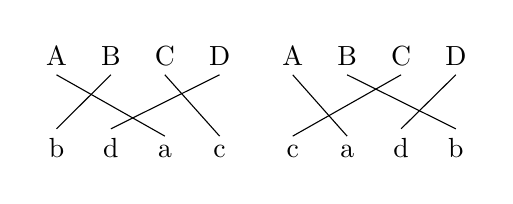
\begin{tikzpicture}[node distance=3cm]
	\usetikzlibrary{matrix}
	\matrix (ex 1) [matrix of nodes,row sep=7mm,column sep=2mm] {
		A & B & C & D \\
		b & d & a & c \\
	};
	\draw (ex 1-1-1.south) -- (ex 1-2-3.north);
	\draw (ex 1-1-2.south) -- (ex 1-2-1.north);
	\draw (ex 1-1-3.south) -- (ex 1-2-4.north);
	\draw (ex 1-1-4.south) -- (ex 1-2-2.north);

	\matrix (ex 2)[matrix of nodes,row sep=7mm,column sep=2mm,right of=ex 1] {
		A & B & C & D \\
		c & a & d & b \\
	};
	\draw (ex 2-1-1.south) -- (ex 2-2-2.north);
	\draw (ex 2-1-2.south) -- (ex 2-2-4.north);
	\draw (ex 2-1-3.south) -- (ex 2-2-1.north);
	\draw (ex 2-1-4.south) -- (ex 2-2-3.north);
\end{tikzpicture}
\end{center}}
\figpostamble
\caption[Visualization of inside-outside alignments.]{Visualization
of inside-outside alignments that are not possible
using bracketing transduction grammar.  Due to the interleaving
words in these configurations, we cannot construct a binary-branching
SCFG that is isomorphic for these strings, although a SCFG with four nonterminals
can produce them.  These are the smallest
impossible configurations in this grammar; as the number of words
in each string increases, so does the number of impossible 
configurations.}
\label{fig:inside-outside-alignment}
\end{figure*}

\subsubsection{Syntax-Based Translation}\label{sec:syntax-based-translation}

In addition to long-distance reordering, a perceived benefit
of SCFG is that 
it allows us to easily incorporate knowledge
based on natural language syntax.
This follows from developments in syntactic 
modeling for ASR \citep{Chelba:1998:acl}.

Often, we will have meaningful linguistic grammars
only for one language.\footnote{Usually
this is the target language \citep{Wu:1998:acl,Yamada:2002:acl}.
This imbalance reflects the fact that many of the
translation systems reported in the literature
are designed to translate into well-studied
languages, such as English, for which we
already have high-quality syntactic parsers.
}
Monolingual syntax resembles our
example fragment CFG (Rules C1-C8).  To use
this monolingual syntax in an SMT model, 
we construct an SCFG where productions 
mirror the known syntax.  In the other language,
we allow arbitrary reorderings of these symbols
\citep{Wu:1998:acl,Yamada:2001:acl}.  The objective 
of such a SCFG is to keep linguistic phrases intact, a property that is often (but not universally) observed in real translation \citep{Fox:2002:emnlp,Wellington:2006:acl-coling}. 
Collectively, models that use linguistic syntax are called
\term{syntax-based models}. 
The example derivation from \figureref{cfg}
is an illustration of this.  

The hypothesis investigated by syntax-based translation
was that reorderings would respect linguistic
syntax in translation.  
Empirical evidence only partially supports this.  
\citet{Fox:2002:emnlp} shows that reordering tends to
respect the boundaries of syntactic phrases, but also
describes some systematic exceptions.  Additional
discrepancies are described by \citet{Wellington:2006:acl-coling}.
The rigidity of full isomorphism at the level of SCFG
productions harms syntax-based translation.  These difficulties
have prompted investigation into more powerful formalisms
for syntactic translation 
\citep{Galley:2004:naacl,Knight:2005:cicling,Galley:2006:acl}.

\subsubsection{Hierarchical Phrase-Based Translation}\label{sec:hiero}

The SCFG models that we have described share
a key weakness of word-based FST-models: they enable only
word-to-word translation, which requires a reordering
decision for each word.  We know that phrase-based models
solve this.  Ideally, we would like to benefit
from the insights behind both hierarchical models and 
phrase-based models.  This is accomplished in hierarchical
phrase-based translation \citep{Chiang:2007:cl,Chiang:2005:acl,Chiang:2005:hlt}.

In this grammar, no linguistic syntax is required. 
A single undifferentiated
non-terminal X is used in the main productions, 
and a maximum of two nonterminals are permitted in
the right-hand size of any rule, just as in bracketing grammar.  
However, unlike a bracketing grammar, 
the right-hand side may also contain a number
of terminal symbols in both languages.  This corresponds
to the basic insight of phrase-based translation, in that 
each rule can represent a mapping between sequences of words.
Essentially, the rules represent phrases that may 
be reordered recursively.  Consider the
following grammar fragment.

\begin{align}
X  \longrightarrow & \textrm{However , }\cidx{\X}{1} \cidx{\X}{2} \textrm{ . }/  
 \textrm{\zh{虽然} }\cidx{\X}{2}\textrm{ , \zh{但} }\cidx{\X}{1} \textrm{ \zh{。}}\tag{H1} \\
X  \longrightarrow & \textrm{under the strong north wind } / 
                    \textrm{\zh{北} \zh{风} \zh{呼啸}} \tag{H2} \\
X \longrightarrow & \textrm{the sky remained clear } /
                   \textrm{\zh{天空} \zh{依然} \zh{十分} \zh{清澈}} \tag{H3} 
\end{align}

\noindent In this grammar, recursivity is captured in 
Rule~H1.  A derivation is illustrated in \figureref{hiero}.

\citet{Chiang:2005:acl,Chiang:2007:cl} showed that this model was
competitive with a standard phrase-based models, outperforming Pharaoh
on standard test sets.

\figpreamble
\begin{figure*}[t]
\figfontsize{\begin{center}
\begin{tikzpicture}[node distance=5cm]
	\tikzstyle{every child} = [level distance=1cm]
	\tikzstyle{edge from parent} = [draw,->]

	\node (scfg 1) [fill=lightgray]{X}{
		child [sibling distance=1cm]{node {However}} 
		child [sibling distance=1cm]{node {,}}
		child [sibling distance=2cm]{node (x1 1){X}{[sibling distance=1.1cm]
			child {node {the}} 
			child {node {sky}} 
			child {node {remained}} 
			child {node {clear}} 
		}}
		child {node {} edge from parent[draw=none]}
		child [level distance=2.5cm,sibling distance=1cm]{node (x2 1){X}{[sibling distance=1.1cm]
			child {node {under}} 
			child {node {the}} 
			child {node {strong}} 
			child {node {north}} 
			child {node {wind}} 
		}}
		child [sibling distance=5mm]{node {.}}
	}; 


	\node (scfg 2) [fill=lightgray,right of=scfg 1,above=1cm]{X}{[sibling distance=1cm]
		child [sibling distance=1.2cm]{node (although){\zh{虽然}}} 
		child [level distance=1.5cm]{node (x2 2){X}{[sibling distance=1.1cm]
			child {node (north) {\zh{北}}} 
			child {node (wind) {\zh{风}}} 
			child {node (howls) {\zh{呼啸}}} 
		}}
		child [sibling distance=7mm]{node (comma){,}}
		child [sibling distance=7mm]{node (but){\zh{但}}}
		child [level distance=3cm,sibling distance=1.2cm]{node (x1 2){X}{[sibling distance=1.3cm]
			child {node (sky) {\zh{天空}}} 
			child {node (still) {\zh{依然}}} 
			child {node (extremely) {\zh{十分}}} 
			child {node (limpid) {\zh{清澈}}} 
		}}
		child {node (period){~~\zh{。}}}
	}; 
	
	\node [anchor=north] at (although.south) {\em Although};
	\node [anchor=north] at (north.south) {\em north};
	\node [anchor=north] at (wind.south) {\em wind};
	\node [anchor=north] at (howls.south) {\em howls};
	\node [anchor=north] at (comma.south) {\em ,};
	\node [anchor=north] at (but.south) {\em but};
	\node [anchor=north] at (sky.south) {\em sky};
	\node [anchor=north] at (still.south) {\em still};
	\node [anchor=north] at (extremely.south) {\em extremely};
	\node [anchor=north] at (limpid.south) {\em limpid};
	\node [anchor=north] at (period.south) {\em .~};
	
	\tikzstyle{scfg connector} = [thin,gray,densely dotted]

	\draw[scfg connector] (scfg 1) ..controls +(1,0.5) and +(-1,0.5) .. (scfg 2);
	\draw[scfg connector] (x1 1) ..controls +(2,0.5) and +(-6,-2) .. (x1 2);
	\draw[scfg connector] (x2 1) ..controls +(1.5,-0.5) and +(-0.5,-2) .. (x2 2);

\end{tikzpicture}
\end{center}}
\figpostamble
\caption{\label{fig:hiero}Visualization of 
hierarchical phrase-based translation.}
\end{figure*}

\subsection{Other Models of Translational 
Equivalence}\label{sec:other-models-of-translational-equivalence}

FST and SCFG models represent a good cross-section of popular
models.  However, a number of models do not
fit these characterizations.

\subsubsection{More Powerful Formalisms}\label{sec:powerful-formalisms}

Moving up the hierarchy of formal languages, 
there are synchronous models based on language formalisms more
powerful than context-free languages.
A good example is tree-adjoining grammar \citep{Joshi:1997:hfl}, which 
we can generalize to synchronous tree-adjoining grammar 
\citep{Shieber:1990:coling}.  Formally,
tree-adjoining grammars are part of a large class of formalisms known
as linear context-free rewriting systems \citep{Vijay-Shanker:1987:acl,Joshi:1991:finlp}.  These
formalisms can parse a restricted subset of context-sensitive
languages in polynomial time.  Much of
the work in this area is currently theoretical.  
However, {\em generalized multitext grammar} \citep{Melamed:2004:acl:gmtg},
which is equivalent to a linear context-free rewriting system,
is the basis of an SMT system \citep{Burbank:2005:tr}.

\subsubsection{Syntactic Phrase-Based Models}\label{sec:syntactic-phrase-based}

Much active research aims to combine the
advantages of hierarchical reordering, syntax, and phrases
\citep{Marcu:2006:emnlp,Galley:2006:acl,Quirk:2005:acl}.
Most of these models employ syntactic reordering models more
complex than those that can be described with SCFG.  The
formal description for several of these models is based on 
{\em tree transducers}, which describe
operations on tree fragments rather than strings.  SCFG
translation can be modeled with tree transducers, although
in general they are strictly more powerful than SCFG.
Systems described using tree transducers are increasingly common, though
many of these are equivalent to SCFG
\citep{Graehl:2004:naacl,Galley:2006:acl,Marcu:2006:emnlp}.
For a good introduction to tree transducers, refer to \citet{Knight:2004:cicling}.

\subsubsection{Alternative Linguistic Models}\label{sec:alternative-syntactic-models}

A wide variety of linguistic theories
are computationally equivalent to CFG, and these can be
used as the basis for translation using SCFG.
Head transducers may be seen as a form of
synchronous \term{dependency grammar} \citep{Alshawi:2000:cl}.  In dependency grammar,
the nodes of the rooted tree which describes the sentence
structure are also the words of the sentence.  It is possible
to derive transformations that will convert many dependency grammars
to context-free grammars, and vice versa \citep{Collins:1999:acl}.  
Therefore, we can construct SCFGs that correspond to 
dependency grammar \citep{Melamed:2003:naacl-main}.
Dependency grammar translation models
are described by \citet{Gildea:2004:emnlp} and \citet{Quirk:2005:acl}.

%%%%% Mathematical Models %%%%%%%%%%%%%%%%%%%%%%%%%%%%%%%%%%%%%%%%%%%%%%%%%%%%%%%%%%%%%%%%%%%%%%%%%%%%%

\section{Modeling Part II: Parameterization}\label{sec:mathematical-modeling}

Translational equivalence models allow us to enumerate
possible structural relationships between pairs
of strings.
However, even within the constraints of a strict
model, the ambiguity of natural language
results in a very large number of possible target sentences for any 
input source sentence.  Our translation
system needs a mechanism to choose between them.

This mechanism comes from our second topic in modeling: \term{parameterization}.
We design a function that allows us to assign a real-valued score 
to any pair of source and target sentences.  The
general forms of these models are similar to those in other machine 
learning problems.  There are a vast number of approaches;
we will only briefly describe the most common ones here.
For more detail, the reader is referred to a general text 
on machine learning, such as \citet{Mitchell:1997:book}.

In typical machine learning problems, we are given 
an input $y \in Y$, and the goal is to 
find the best output $x \in X$.  Note that $x$ and
$y$ may be multidimensional.   We introduce 
a function $f: X \times Y \rightarrow \mathbb{R}$
that maps input and output pairs to a real-valued score
that is used to rank possible outputs.
We introduce the \term{random variables} $\xvar$ and
$\yvar$ which range over the sets $X$ and $Y$,
respectively.  Let $x \in X$ and $y \in Y$
be specific values drawn from these sets. 
The model may be probabilistic,
meaning that we constrain it in one of two ways.
In a \term{joint model}, denoted $P(\xvar,\yvar)$, 
we introduce two constraints.

\begin{eqnarray*} 
&&\sum_{(x,y) \in \{X \times Y\}} P(\xvar=x,\yvar=y) = 1\\
&&\forall_{(x,y) \in \{X \times Y\}}P(\xvar=x,\yvar=y) \in [0,1]
\end{eqnarray*}

\noindent The value $P(\xvar=x,\yvar=y)$ is the
\term{joint probability} of the assignments $\xvar=x$
and $\yvar=y$ occurring, out of all possible
combinations of assignments to these variables.
We will often abbreviate this as $P(x,y)$.

In a \term{conditional model},
denoted $P(\xvar|\yvar)$, we introduce the following constraints.

\begin{eqnarray*}
&&\forall_{y \in Y} \sum_{x \in X} P(\xvar=x|\yvar=y) = 1\\
&&\forall_{(x,y) \in \{X \times Y\}}P(\xvar=x|\yvar=y) \in [0,1]
\end{eqnarray*}

\noindent The conditional probability
$P(\xvar=x|\yvar=y)$, abbreviated $P(x|y)$, 
is simply the probability of the 
assignment $\xvar=x$, given that the assignment
$\yvar=y$ is fixed. In this case, we assume that
knowledge of the value assigned to $\yvar$ will
help us determine the assignment to $\xvar$.

These constraints represent the 
\term{distribution} of finite probability mass 
across all combinations of assignments to $\xvar$ and $\yvar$.  
In many machine learning problems,
it is not unusual for the input set $Y$ to be
complex.  Often, the set $X$ of possible outputs 
is a small, finite set of \term{labels} or \term{classes}
and our goal is simply to find the best 
\term{classification} of the input.
This is not the case in SMT, where our input
$\fvar$ ranges over ${V_F}^*$ and our output $\evar$ ranges
over ${V_E}^*$. We will usually expand our definition of
the output to include the decisions made by our
translational equivalence model defining the 
relationship between $\fvar = f_1^J$ and 
$\evar = e_1^I$.  We denote this structure
using the variable $\dvar = d_1^M \subset D$.
Recall that $D$ is a set of transitions in the 
case of FST models (\sectionref{finite-state-models})
and a set of grammar productions in the case of 
SCFG models (\sectionref{hierarchical-models}); in 
other words, $D$ is simply a set of rules. In the SMT
problem, we are given an input $\fvec$ and we are
interested in finding multidimensional ``class'' $(e_1^I, d_1^M)$
drawn from a domain that is exponential in the size of the input.
This problem is known as \term{structured classification}
or \term{structured prediction} \citep{Taskar:2004:thesis}.
Note that the set $\dvec$ of derivations exactly defines
$\evec$ for a given input $\fvec$, and we could simply
denote the label using $\dvec$; we use
$(\evec,\dvec)$ to remind us of our ultimate goal.  For
notational purposes we also
define a predicate $Y(\evec,\dvec)$ that is true
when the derivation $\dvec$ yields $\evec$, and false otherwise.

The mathematical function that we are truly interested
in is $P(\evar|\fvar)$.  This function
ignores the derivation of the output.  However, these models usually
define multiple structures that
can relate the same pair $(e_1^I,f_1^J)$.  The value of 
$P(\evar|\fvar)$ is therefore obtained by summing the probabilities
of all derivations that yield $\evar$.

\begin{equation}
P(\evar|\fvar) = \sum_{\dvar : Y(\dvar,\evar)} P(\evar,\dvar|\fvar)
\end{equation}

\noindent Unfortunately, computation of this sum involves
exponential complexity in both 
FST \citep{Brown:1993:cl} and
SCFG models \citep{Melamed:2004:acl:smtbyp}.  Therefore
we will use the simpler function $P(\evar,\dvar|\fvar)$
for classification.
We can view the classification problem as one in which
the decoder produces candidate labels according to
our translational equivalence model, and the parameterization
of the model determines the rank of candidates.  Usually these
tasks are integrated, but not necessarily 
(see \sectionref{reranking}).

Although the function $P(\evar,\dvar|\fvar)$ ranges over
discrete sets, these sets are very large or even infinite.  
This poses both practical
and theoretical problems.  There is no efficient way to
enumerate the function.  Furthermore, we will never have
enough training data to reliably learn what its values
should be.  The goal of mathematical 
modeling, then, is to {\em parameterize} the function in such 
a way that we can efficiently and reliably learn it.  
There are a number of ways to accomplish this.
We describe \term{generative models}
in \sectionref{generative-models} 
and \term{discriminative models}
in \sectionref{discriminative-models}.

\subsection{Generative Models}\label{sec:generative-models}

We begin our discussion of generative models by 
introducing some statistical machinery.  Later in the
section, we will illustrate this with an example.

One method of manipulating probabilistic
models is through use of the chain rule.

\begin{equation}
P(\xvar,\yvar) = P(\xvar|\yvar) P(\yvar)
\end{equation}

\noindent Generative models decompose 
$P(\xvar|\yvar)$ using Bayes' rule, which we derive
using the chain rule and a bit of algebra 
as shown in Equation~\ref{eq:bayes-general}.

\begin{equation}\label{eq:bayes-general}
P(\xvar|\yvar) = \frac{P(\xvar,\yvar)}{P(\yvar)} = 
\frac{P(\yvar|\xvar)P(\xvar)}{P(\yvar)} 
\end{equation}

\noindent Applying Bayes' rule to our structured
classification problem, we arrive at the following
decomposition:

\begin{equation}\label{eq:bayes}
P(\evar,\dvar|\fvar) = \frac{P(\fvar,\dvar|\evar)P(\evar)}{P(\fvar)}
\end{equation}

\noindent In decoding we can 
ignore the denominator $P(\fvar)$
because it is constant for any input $f_1^J$.  Therefore, we do not
need to consider this model any further and we can focus on 
$P(\fvar,\dvar|\evar)$ and $P(\evar)$.
The decomposition was inspired by its successful
use in automatic speech recognition
\citep{Brown:1990:cl}.

In SMT we call $P(\evar)$ the \term{language model}
and $P(\fvar,\dvar|\evar)$ the \term{translation model}.
Note that while our objective is to discover 
$e_1^I$ given $f_1^J$, we actually model the reverse.
This originated with the IBM 
system, and it is for this reason that IBM Model
4 is described as a translation from $e_1^I$ to
$f_1^J$ as we saw in \sectionref{word-based-models}.
The advantage of this over modeling 
$P(\evar,\dvar|\fvar)$ directly is that we can apply two
independent models to the disambiguation 
of $\evar$ \citep{Brown:1990:cl}. 
This is beneficial because our estimates for each model 
are errorful.  By applying them together 
we hope to counterbalance
their errors.

In fact, we can think of the language model $P(\evar)$ as
a stochastic model that generates target language sentences,
and the translation model $P(\fvar,\dvar|\evar)$ as a
second stochastic process that ``corrupts'' the target
language to produce source language sentences.
This idea was suggested by Weaver.

\begin{quotation}
\noindent One naturally wonders if the
problem of translation could conceivably be 
treated as a problem in cryptography.  When I 
look at an article in Russian, I say: ``This 
is really written in English, but it has been 
coded in some strange symbols.  I will now 
proceed to decode.'' \citep{Weaver:1955:mt}
\end{quotation}

\noindent Weaver makes analogy to information theoretic
work on signal transmission over a physical medium,
called the \term{noisy channel} problem.  
It is illustrated in \figureref{noisy-channel}.
Following Weaver, the
process to recover $e_1^I$ is called \term{decoding}.

\figpreamble
\begin{figure*}[t]
\figfontsize{\begin{center}
\begin{tikzpicture}
	\node [draw] (source) {$\Pe$};
	\node [right of=source,node distance=1.5cm] (e) {$e_1^I$};
	\node [right of=e,node distance=4cm] (f) {$f_1^J$};
	\draw [->] (source) -- (e);
	\draw [->,snake=snake,line after snake=1mm,line before snake=1mm] (e) -- (f);
	\node [fill=white,right of=e,node distance=2cm] (channel) {$\Pfe$};
	\node [anchor=south,above=2mm] at (source.north) {source};
	\node [anchor=south,above=2mm] at (channel.north) {noisy channel};
\end{tikzpicture}
\end{center}}
\figpostamble
\caption[The noisy channel model of sentence pair generation.]{\label{fig:noisy-channel}The noisy channel model 
of sentence pair generation.  The source model $P(\e)$ 
produces $e_1^I$, which is then transformed
by the channel model $P(\f|\e)$ to produce $f_1^J$.  
If we are given only $f_1^J$, we can try to deduce an $e_1^I$
using our knowledge of both models.}
\end{figure*}

\subsubsection{Language Models}\label{sec:language-models}

In language modeling, our goal is to find a tractable
representation of the function $P(e_1^I)$.
Generative models use probabilistic tools for
this.  One of these is chain rule, which allows us
to write the following.

\begin{align}
P(e_1^I) = \prod_{i=1}^I P(e_i|e_1^{i-1})\label{eq:lm-full}
\end{align} 

\noindent This equation tells us that the conditional probability
of the sentence $e_1^I$ is
simply the product of many small probabilities, each
of which corresponds to a single word.

Equation~\ref{eq:lm-full} helps to simplify our
problem, but not completely.  For instance, the distribution
$P(e_I|e_1^{I-1})$ assigned to the last word of the sentence
contains nearly as many terms as $P(e_1^I)$ itself.
In order to simplify the model even further
we introduce the idea of \term{conditional
independence}.  When we say that a variable $\xvar$ is
conditionally independent of $\yvar$, we mean that
$P(\xvar|\yvar) = P(\xvar)$.  In other words, conditional
independence means that knowing the value of $\yvar$ 
does not affect the probability distribution 
of $\xvar$.  By making independence assumptions
about our data, we can drop enough 
terms from our functions that they become 
tractable.  The obvious danger, of course, is that 
if we make too many or wrong independence assumptions,
our resulting probability distributions will be incorrect.
This is a constant danger in SMT modeling.  In general,
nearly any independence assumption will be unrealistic; 
our hope is that they are approximately close enough
to that it will not harm our results.  
Making conditional independence assumptions 
is a matter of art and pragmatism.

In language modeling, the simplest assumption we
can make is that the probability of word $e_i$ is
conditionally independent of all but the $n-1$ preceding
words $e_{i-n}^{i-1}$.  We call $e_{i-n}^i$ an {\em $n$-gram}
and the language model based on this independence assumption is an \term{$n$-gram
language model}.  We assume without loss of generality that
the first word $e_1$ is preceded by $n-1$ distinguished
start symbols not in $V_E$.

We will use the notation $P_\delta(\xvar|\yvar)$ to represent
the distribution $P(\xvar|\yvar)$ that has been rewritten
to include only elements of $\yvar$ on which $\xvar$ is
conditionally dependent.  Using this notation,
we can rewrite Equation~\ref{eq:lm-full} as an $n$-gram
model.

\begin{align}
P(e_1^I) = \prod_{j=1}^I P_\delta(e_i|e_1^{i-1}) = \prod_{j=1}^I P(e_i|e_{i-n}^{i-1})\label{eq:ngram-lm}
\end{align} 

\noindent Most language models take this form,
inherited from SMT's roots in speech recognition.
The discussion of $n$-grams barely scratches the surface
of language modeling, which is a full topic in its own
right, well beyond the scope of this paper.  
For a good overview, refer to a text on speech
recognition, such as \citet{Jelinek:1998:book}.

Language modeling has not received much 
special attention in the 
SMT community, which has preferred to focus on the more 
specialized translation models.  However, it continues
to be an active area of research, especially in the
speech recognition community.  Most SMT systems simply
borrow models that were popularized for speech.  However,
there is little doubt that better language modeling leads
to better translation
\citep{Eck:2004:lrec,Kirchhoff:2005:wpt,Och:2005:wpt,Zhang:2006:emnlp,Brants:2007:emnlp-conll}.
A few syntax-based models 
are constructed to take advantage of syntactic language
models based on context-free grammars
\citep{Wu:1998:acl,Charniak:2003:mtsummit,Marcu:2006:emnlp}.

\subsubsection{Translation Models}\label{sec:translation-models}

Taking advantage of the statistical machinery that we have
introduced, we now turn to the {\em translation model}
$P(f_1^J,d_1^M|e_1^I)$.  As we have seen, we can use the 
chain rule to decompose this into a series of smaller models.

\begin{align}
P(f_1^J,d_1^M|e_1^I) = \prod_{j=1}^J P(f_j|f_1^{j-1},d_1^M,e_1^I) \times
\prod_{m=1}^M P(d_m|d_1^{m-1},e_1^I) \label{eq:generative}
\end{align} 

\noindent This equation tells us that the conditional probability
of the pair $(f_1^J,d_1^M)$ with respect to $e_1^I$ is
simply the product of many small probabilities, each
of which corresponds to a single action taken by our
translational equivalence model.  Thus, in our FST
model, there is a probability for each transition in
each transducer; in our SCFG model, there is a probability
for each production.  Using our notation for conditional independence,
we can now rewrite Equation~\ref{eq:generative}.

\begin{equation}
	P(f_1^J,d_1^M|e_1^I) = \prod_{j=1}^J P_\delta(f_j|f_1^{j-1},d_1^M,e_1^I) \times
	\prod_{m=1}^M P_\delta(d_m|d_1^{m-1},e_1^I) 
\end{equation} 

\noindent Assuming that we have made strong enough
independence assumptions, each distribution on the right
side of this equation 
contains a sufficiently small number of terms that we 
can actually learn them.  At runtime,
we will simply look up the values associated with
the terms and use them to compute the function.
Each of these values is a \term{parameter} of our model.
In other words, a parameter is an element of the 
smallest distribution that we represent in
our models---a distribution that we do not represent
as a function of other distributions. We will use 
$p(x,y)$ or $p(x|y)$ to denote parameters.  We already
saw a parameter in the section on language modeling:
$p(e_i|e_{i-n}^{i-1})$ was a parameter.

We do not have space to describe all of the 
parameterizations that have been proposed for 
even the small selection of translational equivalence
models we described in \sectionref{translational-equivalence-models}.  
However, we will use a slightly simplified version of
IBM Model~4 as an example to illustrate parameterization of generative
models.  Recall the steps of this model.

\begin{enumerate}
	\item Each target word $e_i$ selects a fertility $\phi_i$ and copies itself $\phi_i$ times.
	\item Each copy of each target word is translated to a single source word.
	\item The source words are reordered into their final positions.
\end{enumerate}

Let us now take a look a parameterization of this model.  We know that
we want to assign a probability to each step taken by the model.  Therefore,
we will need a {\em fertility probability}, a {\em word translation probability},
and some probability to control the reordering, which we call a {\em distortion
probability}.

Fertility is simple.  We can make it conditionally
dependent on the word identity.  We define the
fertility probability for word $e_i$ 
by the parameter $p(\phi_i|e_i)$.  We can think of
this as the probability that a human translator
would choose $\phi_i$ source words to translate the 
target word $e_i$.

Word translation is equally simple if we limit ourselves to the identities of
the words being translated.  Let  $\tau_{i,k} \in V_F$ be the translation
of the $k$th copy of $e_i$.  The word translation probability is then
$p(\tau_{i,k}|e_i)$.  This is quite intuitive.  We can think of it
as the probability that a translator, when presented with word $e_i$, 
will choose to translate it using word $\tau_{i,k}$.

Let $T$ denote the set of all random variables 
$T = \{\tau_{i,k}:0 \leq i \leq I, 0 \leq k \leq \phi_i\}$ representing 
target word translations.

Modeling the reordering step is a bit more complicated.  We will
use two parameters to control this.  The first parameter controls
the placement of the {\em first} word generated by $e_i$, $\tau_{i,1}$.
Let random variable $\pi_{i,1}\in [1,J]$ denote its final position.
IBM Model~4 models this
according to the distribution $p(\pi_{i,1}-\odot_{i-1}|C_E(e_{i-1}),C_F(\tau_{i,1}))$.
Here, $\pi_{i,1} \in [1,M]$ represents the final absolute location of the translated
word and $\odot_{i-1} = \frac{1}{k} \lceil \sum_{k=1}^{\phi_{i-1}} \pi_{i-1,k} \rceil$ 
represents the average location of all translations of
$e_{i-1}$.  In other words, we make its position dependent on the positions
of the previously translated word.  The functions $C_E : E \rightarrow [1,K]$ 
and $C_F : F \rightarrow [1,K]$ partition the vocabularies $V_E$ and $V_F$ onto suitably
small sets of $K$ classes to avoid the sparseness that would arise from conditioning
on the words themselves \citep{Brown:1992:cl,Och:1999:eacl}.

Just as we condition the positioning of the first translated word $\tau_{i,1}$
on the position of the translations of the adjacent target word, we condition
the positioning of $\tau_{i,k}$ on $\pi_{i,k-1}$.  Let this be controlled by the distribution  $p(\pi_{i,k}-\pi_{i,k-1}|C(\tau_{i,k}))$. 
We use $\Pi$ to denote the set of all random variables 
$\Pi = \{\pi_{i,k}:0 \leq i \leq I, 0 \leq k \leq \phi_i\}$ representing word positions.

We can now show the complete parameterization of the IBM Model~4.\footnote{For
simplicity, we leave out the parameterization of null translation.}

\begin{equation} \label{eq:models45} 
\begin{array}{lll}
\displaystyle \Pfe = \sum_{T,\Pi} & \displaystyle \prod_{i=0}^I p(\phi_i|e_i) \times & {\rm fertility} \\
 \nonumber               & \displaystyle ~~\prod_{i=0}^I \prod_{k=1}^{\phi_i} p(\tau_{i,k}|e_i) \times & {\rm translation}\\
 \nonumber               & \displaystyle ~~~~\prod_{i=0}^I p(\pi_{i,1}-\odot_{i-1}|C_E(e_{i-1}),C_F(\tau_{i,1})) \times & {\rm distortion~for~}\tau_{i,1}\\
 \nonumber               & \displaystyle ~~~~~~\prod_{i=0}^I\prod_{k=2}^{\phi_i} p(\pi_{i,k}-\pi_{i,k-1}|C(\tau_{i,k})) \times & {\rm distortion~for~}\tau_{i,k}, k>1\\
\end{array}
\end{equation}

As we can see from this discussion, 
the parameterization of generative models is closely
tied to the form of the underlying translational equivalence model.
However, many of these parameters have obvious analogues in other models.
For instance, phrase-based models are parameterized using
{\em phrase translation probabilities}, which apply to pairs of phrases,
and are analogous to word translation probabilities
\citep{Marcu:2002:emnlp,Koehn:2003:naacl}.
Numerous other parameterizations of distortion have been proposed for FST models
\citep{Al-Onaizan:2006:acl-coling,Vogel:1996:coling,Och:2000:coling,Toutanova:2002:emnlp,Lopez:2005:wpt,DeNero:2007:acl}.  
The parameterization of SCFG models follows a similar pattern of diversity.

\subsection{Discriminative Models}\label{sec:discriminative-models}

Generative models are useful
in decoding (\sectionref{decoding}) because they
correspond so closely to the translational
equivalence models that define the search space.
However, there are tradeoffs.  As we have seen,
 to make them both theoretically well-founded and 
tractable, we must make very strong independence
assumptions.  This means that the
information that we can bring to bear at each individual
decision point is very limited.  For instance, we 
are generally limited to translation between small
numbers of words in each sentence, although we 
expect in principle that knowledge of all words
in a source sentence may help us translate any particular word.
Using generative models, there is no tractable 
mechanism to represent this.

We can bring additional context into modeling by moving from 
generative to \term{discriminative} models.  In SMT,
a popular form for this is \term{log-linear}
modeling \citep{Berger:1996:cl,Och:2002:acl}.\footnote{
In the more general literature this is often simply 
called a {\em linear model}.}  
The introduction
of log-linear models to SMT follows from
their increasing use in NLP  
\citep{Berger:1996:cl,Ratnaparkhi:1998:thesis,Smith:2006:thesis},
and reflects general trends in machine learning.

Log-linear models define a relationship between 
a set of $K$ fixed \term{features} $h_1^K(\evar,\dvar,\fvar)$ 
of the data and the function $P(\evar,\dvar|\fvar)$
that we are interested in.  A feature can be 
any function $h : E^* \times D^* \times F^* \longrightarrow [0,\infty)$,
that maps every pair of input and output strings 
to a non-negative value.  An example of a 
feature might be the number of times a particular
word pair $(e_i,f_j)$ appears in the data 
\citep{Och:2002:acl}; the number of phrases
in a segmentation of $\evec$ \citep{Koehn:2004:pharaoh}; 
or the logarithm of the probability defined by  
a generative model (or even one of its distributions)
from the previous section.  Most features used in 
SMT to date have taken the latter form.  
Log-linear models take the form of Equation~\ref{eq:loglinear}.

\begin{equation}
P(\evar,\dvar|\fvar) =
\frac{\exp \sum_{k=1}^K \lambda_k h_k(\evar,\dvar,\fvar)}{ \sum_{\evar',\dvar':Y(\evar',\dvar')} \exp \sum_{k=1}^K \lambda_k h_k(\evar',\dvar',\fvar)}\label{eq:loglinear}
\end{equation}

\noindent The daunting normalization factor in the denominator
is required only to make the function a well-formed 
probability.  Fortunately, we can ignore it during decoding
because it constant for any given $f_1^J$.  Its computation
may or may not be required during parameter estimation, depending
on the algorithm.

The log-linear model defined in Equation~\ref{eq:loglinear}
has $K$ parameters, $\lambda_1^K$.\footnote{Confusingly,
in the general literature this is sometimes
called a {\em parameter-free} model.  It is also known as
a {\em distribution-free} model, which can be understood
from the fact that the normalization is not 
strictly required.}  These are called 
\term{feature weights} or \term{model scaling factors}.
They determine the contribution of a feature to the overall 
value of $P(\evar,\dvar|\fvar)$.  Ideally, each parameter
would indicate the pairwise correspondence between the
feature and the output probability.  A positive value 
$\lambda_k$ should indicate that the feature
$h_1^K(\evar,\dvar,\fvar)$ correlates with  
$P(\evar,\dvar|\fvar)$; a negative value should indicate
an inverse correlation; and a value near zero should
indicates that the feature is not a useful predictor of
$P(\evar,\dvar|\fvar)$.  However, in practice, if two features
are highly correlated with each other, an estimator might distribute the
weight in any fashion between them.  If a feature is
uncorrelated with the output, then the estimator might
assign an arbitrary weight to it.  This complicates
parameter estimation and motivates the task of {\em feature
selection}, which seeks to identify the smallest set
of the most predictive features.  Feature selection is
a very open problem in SMT.

Note that Equation~\ref{eq:bayes} corresponds to a 
special case of Equation~\ref{eq:loglinear}
when the following conditions hold.

\begin{eqnarray*}
&&K = 2 \\
&&\lambda_1 = \lambda_2 = 1 \\
&&h_1(\e,\f) = \log P(\fvar,\dvar|\evar)\\
&& h_2(\e,\f) = \log P(\evar)
\end{eqnarray*}

\noindent Log-linear models \term{discriminate}
between different possible values $e_1^I$ when presented
with a particular $f_1^J$.  In contrast
with generative models, there is no requirement that we
assign a single probability to every element of data.  
We may assign multiple probabilities to an element or none
at all.  In fact, the values that we assign are not
required to be well-formed probabilities at all---
the normalization factor in Equation~\ref{eq:loglinear}
takes care of this for us.
In particular, we are not required to define
probabilities for our input data as we do in 
generative models.  Because we are 
freed from the constraints of Bayes' rule, features 
can be overlapping---we could, for instance, use 
several of the generative models discussed previously,
even though each of them will have a different 
explanation of each word in the target language.
In principle, any other model of
$\Pe$, $\Pfe$, $\Pef$, or $\Pefj$, or combination
thereof, can be a feature.\footnote{A 
justification for using log-linear models in this way was that  
a system based on $\Pe \cdot P(\evar,\dvar|\fvar)$ worked nearly as well as 
$\Pe \cdot P(\fvar,\dvar|\evar)$ in empirical studies, even though the former
cannot be theoretically motivated using Bayes' rule
\citep{Och:1999:emnlp,Och:2002:acl}.  Beginning with \citep{Koehn:2004:amta},
many systems use both \citep{Simard:2005:hlt-emnlp,Marcu:2006:emnlp,Chiang:2007:cl}.
It is not clear if this is beneficial \citep{Lopez:2006:amta}.}  A 
popular technique is to simply take the summed logarithm of
all instances of a particular distribution in an underlying 
generative model.  This yields a small number of features,
usually less than ten.  Another important feature of
most models is the {\em word count} or {\em word penalty}
feature, which is the number of words in the
target sentence.  Its weight therefore controls
target sentence length.\footnote{\citet{Lopez:2006:amta} found this
feature to be quite important.  This is partly due to the use
of evaluation metrics that are very sensitive to length
\textsection\ref{sec:evaluation}.}

Discriminative modeling is powerful because it 
frees us from the generative modeling requirement
that each term must conform to an event in our
translational equivalence model, which is often
chosen for computational reasons rather than for
its ability to distinguish between good 
translations.  This allows
us to define arbitrary features that may help to 
improve translation.  The primary art in 
discriminative modeling is defining useful features.  
However, with some exceptions this area has not
been fully explored
\citep{Och:2003:jhu,Och:2004:naacl,Marcu:2006:emnlp,Liang:2006:acl-coling,Venugopal:2007:hlt-naacl}.
Many models use little more than a word penalty feature and a
small set of generative features that can be traced directly to 
the IBM Models.

%%%%% Parameter Estimation %%%%%%%%%%%%%%%%%%%%%%%%%%%%%%%%%%%%%%%%%%%%%%%%%%%%%%%%%%%%%%%%%%%%%%%%%%%%%

\section{Parameter Estimation}\label{sec:parameter-estimation}

Once we have defined $\Pedf$, we need to 
assign values to its parameters, 
the actual values that are used to compute it.
We call this \term{parameter estimation}.
In SMT, we use a parallel corpus as input
to a machine learning algorithm in order
to learn the parameter values.  Broadly speaking, 
we can say that SMT relies on \term{supervised learning},
because we are given samples of input/output pairs.

Most SMT systems use a log-linear model of $\Pedf$ that
incorporates generative models as feature functions.
Before we can learn the parameters of 
the log-linear model, we must fix values of the feature
functions, including any generative models used as features.
This means that we must first estimate any underlying
generative models independently, and then separately estimate
the parameters of the log-linear models.  An method for
iteratively estimating both is presented by \citet{Fraser:2006:acl-coling}.

We describe parameter estimation for generative
models in \sectionref{parameter-estimation-generative}.
We will then discuss the important concept of word
alignment in \sectionref{word-alignment}.
Finally, we describe parameter 
estimation for log-linear models in
\sectionref{log-linear-estimation}.



\subsection{Parameter Estimation in Generative
Models}\label{sec:parameter-estimation-generative}

An example parameter from our generative models
is the translation probability $p($\zh{风}$|$wind$)$.
Our model says that we will use this value whenever
we translate the word ``\zh{风}'' as ``wind''.  To
estimate this parameter, we turn to our parallel
corpus.

One way to capitalize on our data comes to us
from statistical estimation theory.  We assume
that the parallel corpus was produced by our model 
using the unknown, true parameter values.
Our goal, then, is to \term{estimate} those values
so that our estimates are as close as possible 
to the true ones.

If we denote our training data as $C \subset \{E^* \times F^*\}$, 
the complete set of parameters as $\Theta$, and the probability 
(or likelihood) of $C$ under parameter set $\Theta$ as 
$P_\Theta(C)$, then our goal is to choose $\Theta$ that
satisfies Equation~\ref{eq:mle}.

\begin{equation}\label{eq:mle} 
\Theta = \argmax_{\hat{\Theta}} P_{\hat{\Theta}}(C).  
\end{equation}

\noindent Parameter estimation, then, is equivalent to finding 
the maximum of a function (the \term{objective function})
---in this case, the \term{likelihood} function $P_\Theta(C)$.  
We call this \term{maximum likelihood estimation} (MLE).  
The parameter set $\Theta$ that satisfies the
maximization problem in Equation~\ref{eq:mle}
is the \term{maximum likelihood estimate}.  
This is not the only
possible objective function, but it is the one
that is typically used for generative models.  We will
discuss a different objective function in 
\sectionref{minimum-error-rate-training}.

\subsubsection{Learning Word Translation Probabilities}
\label{sec:unsupervised-learning-generative}

Recall that in our generative models, each probability
is tied to a single decision taken by the model.
MLE is easy when we can observe all of these decisions.
Consider a very simple model, the coin-flip model.
In this model, we have a coin that comes up
heads with probability $p(h)$.  We do not know $p(h)$
and we would like to guess what it is.  If we have 
access to the coin itself, we can flip it a number 
of times and see how many times each side comes up.  
Suppose that we flip the coin a number of times, and
we count the number of times it comes up heads, which
we denote $\#(h)$.  The total number of flips is the
sum of the number of heads and tails, $\#(h+t)$.
Most people know intuitively
that the value for $p(h)$ should be $\#(h)/\#(h+t)$.  In fact,
we can show analytically that this relative 
frequency estimate corresponds to the MLE.
The accuracy of MLE depends crucially on the
number of examples---we
can see that if we flip the coin only once, then the
only possible outcomes are $p(h)=1$ and $p(h)=0$, either
of which is likely to be far from the true value of
the parameter.  This
issue has not received much attention in SMT,
although \citet{Foster:2006:emnlp} show that 
methods to {\em smooth} poorly estimated probabilities
can improve performance.\footnote{A discussion of smoothing
is highly relevant, as it is to most NLP problems, but
well beyond the scope of this paper.  
\citet{Chen:1998:tr}, \citet{Manning:1999:book}, and 
\citet{Jurafsky:2000:book}
and are good starting points.}\footnote{In fact, the unsmoothed values 
used by most phrase-based models are so
imprecise that they can be stored in four bits without
loss of performance \citep{Och:2005:wpt,Federico:2006:smt}.
}


Now suppose that we wish to estimate the
parameters of a word-based generative translation
model.  If we had access to an alignment---such as the one 
depicted in \figureref{alignment}---for every sentence in our corpus,
then it would be easy to count the fertility,
substitution, and distortion outcomes for each word, 
and we could estimate our parameters as
easily as we did in the coin-flipping model.
For instance, if we saw the word ``wind'' $\#($wind$)$
times, and it was aligned to the word ``\zh{风}''
$\#(a($\zh{风}$,$wind$))$ times, 
then we would compute $p($\zh{风}$|$wind$) = \#(a($\zh{风}$,$wind$))/\#($wind$)$.

It is not that easy, however.  The data that we collect
from the real world contains only sentence pairs, not alignments.\footnote{
In fact, we have even glossed over the conversion of raw text data
to sentence pairs, which is not an entirely trivial problem 
\citep{Church:1993:cl-align,Smith:2002:emnlp}.}
So, while we can 
see that ``wind'' and ``\zh{风}'' both \term{cooccur} 
in many of these sentence pairs, we cannot see how many times 
they are actually aligned to each other.   We can make
some estimates based only on cooccurrence---for instance,
we will estimate $p(f|e)=0$ for words $f$ and
$e$ that never cooccur in our training data.  How can
we estimate the probability for words that {\em do} cooccur?

One solution to this problem is to automatically generate
an alignment, and then to use this alignment as
our training data for maximum likelihood estimation. 
We will describe word alignment methods in 
\sectionref{word-alignment}.  Alternatively,
we need a method to estimate our parameters that will work 
even when we cannot explicitly count all of the decisions
that we are interested in.  Since we 
will not be able to directly observe the outcome
of each decision made by our model, 
we can view the learning of 
the associated parameters as a form of 
\term{unsupervised learning}.
A method that is commonly used to solve this problem in SMT is the 
Expectation-Maximization (EM) algorithm \citep{Dempster:1977:rss}.  
It works by substituting
observed counts of events with \term{expected counts}.
Although we cannot actually observe the number of times that 
``wind'' aligns to ``\zh{风}'', we can compute the
expected number of times that this happens if we
have some initial value for $\Theta$, which we
will call $\Theta_0$.  Let $\Theta_0$
be random, uniform, or initialized from some
simpler model.  We can then compute the 
expected count of the event
$E(a(\textrm{\zh{风}},$wind$))$ in any particular
sentence pair $(\e,\f)$ as follows.

\begin{equation*}
E(a(\textrm{\zh{风}},\textrm{wind})) = \frac{P_{\Theta_0}(a(\textrm{\zh{风}},\textrm{wind}), \fvec|\evec)}
{P_{\Theta_0}(\fvec|\evec)}
\end{equation*}

\noindent In other words, we compute all possible alignments
between $\fvec$ and $\evec$,
and their probabilities under $\Theta_0$.  We then 
sum the probability of those alignments that contain
the decision that we are interested in, and divide this
by the summed probability of all possible alignments.  This
gives a fractional expected probability that the event 
occurred.  If we apply
this method to all parameters over the entire corpus,
we can produce a new estimate, $\Theta_1$.  Under
certain conditions this offers the minimal guarantee that
$P_{\Theta_1}(C) > P_{\Theta_0}(C)$.  Thus, it works by
{\em hill-climbing}, or constantly improving its estimate
of $\Theta$.  We can define EM according to the following 
recursion, for our observed training data $C$ and unknown 
alignment data $D$.

\begin{equation}
\Theta_i = \argmax_{\hat{\Theta}} P_{\hat{\Theta}}(C,E_{\Theta_{i-1}}(D))
\end{equation}

\noindent The EM algorithm does not, 
in general---and in particular for most SMT models---
guarantee convergence to a globally
optimal value for $\Theta$.  In fact, it depends 
crucially on a good initial estimate $\Theta_0$
to avoid a poor local maximum.  A method for
generating this estimate for the IBM Models is 
sketched in \sectionref{word-alignment}.
Despite the various difficulties in using EM, it
has been applied to a variety of other NLP problems 
\citep{lari:1990:csl,merialdo:1994:cl}.

A full discussion of the EM
algorithm is beyond the scope of this paper.  
For a more detailed overview, refer to
\citet{Dempster:1977:rss}.  For a full account 
of the analytical solution to the EM algorithm
in the case the IBM Models, refer to 
\citet{Brown:1993:cl}.

\subsubsection{Learning Phrase Translation Probabilities}
\label{sec:supervised-estimation-generative}

In order to train the parameters of a phrase-based model 
we must have access to a \term{phrase-to-phrase alignment}.
EM for phrase-based models involves many approximations
and tradeoffs \citep{Marcu:2002:emnlp,DeNero:2006:smt,Birch:2006:smt}.
A pragmatic solution is to generate
a word alignment (\sectionref{word-alignment}), 
and then count all phrases that
are consistent with the alignment 
\citep{Och:1999:emnlp,Koehn:2003:naacl}.  We then 
compute the MLE using the hypothesized phrases as our
observed events.  We say that a bilingual 
phrase is consistent with a word alignment if no 
word inside the phrase is aligned to any word outside
the phrase---in other words, the phrase contains the
transitive closure of some set of nodes in the bipartite
alignment graph.  This is illustrated in 
\figureref{phrase-learning}.

\figpreamble
\begin{figure*}[t]
\figfontsize{\begin{center}
\begin{tikzpicture}
	\matrix (alignment)[nodes={anchor=east,minimum height=12pt},matrix of nodes]{
		However \\
		, \\
		the \\
		sky \\
		remained \\
		clear \\
		under \\
		the \\
		strong \\
		north \\
		wind \\
		. \\
		|[rotate=-90,anchor=west]| ~ & 
		|[rotate=-90,anchor=west]| \zh{虽然}~{\em (Although)} & 
		|[rotate=-90,anchor=west]| \zh{北}~{\em (north)} & 
		|[rotate=-90,anchor=west]| \zh{风}~{\em (wind)} & 
		|[rotate=-90,anchor=west]| \zh{呼啸}~{\em (howls)} & 
		|[rotate=-90,anchor=west]| \zh{,}~{\em (,)} & 
		|[rotate=-90,anchor=west]| \zh{但}~{\em (but)} & 
		|[rotate=-90,anchor=west]| \zh{天空}~{\em (sky)} & 
		|[rotate=-90,anchor=west]| \zh{依然}~{\em (still)} & 
		|[rotate=-90,anchor=west]| \zh{十分}~{\em (extremely)} & 
		|[rotate=-90,anchor=west]| \zh{清澈}~{\em (limpid)} & 
		|[rotate=-90,anchor=west]| ~~\zh{。}~{\em (.)} \\
	};
	\tikzstyle{alignment grid} = [gray,thin]
	\foreach \e in {1,...,12}{
		\draw[alignment grid] (alignment-\e-1.north -| alignment-13-2.south) -- (alignment-\e-1.north -| alignment-13-12.north);
	}
	\draw[alignment grid] (alignment-12-1.south -| alignment-13-2.south) -- (alignment-12-1.south -| alignment-13-12.north);

	\foreach \f in {1,...,12}{
		\draw[alignment grid] (alignment-13-\f.north |- alignment-12-1.south) -- (alignment-13-\f.north |- alignment-1-1.north);
	}
	
	\tikzstyle{phrase} = [rounded corners,fill=black,draw,fill opacity=0.1];
	\foreach \ej/\ek/\fj/\fk  in {
			2/2/6/6, 
			4/4/8/8, 
			5/5/9/9, 
			6/6/11/11/,
			9/9/5/5,
			9/8/5/5,
			9/7/5/5,
			10/10/3/3,
			11/11/4/4,
			12/12/12/12,
			5/4/8/9,
			5/3/8/9,
			6/4/8/11,
			6/3/8/11,
			6/5/9/11,
			7/4/8/11,
			7/3/8/11,
			7/5/9/11,
			8/4/8/11,
			8/3/8/11,
			8/5/9/11,
			11/10/3/4,
			11/9/3/5,
			11/8/3/5,
			11/7/3/5,
			12/1/2/12,
			11/1/2/11}{
		\path [phrase] (alignment-\ej-1.south -| alignment-13-\fj.south) 
			rectangle (alignment-\ek-1.north -| alignment-13-\fk.north);
	}
	\tikzstyle{aligned word} = [circle,fill=black]
	\foreach \e/\f in {1/2, 1/7, 2/6, 4/8, 5/9, 6/11, 9/5, 10/3, 11/4, 12/12}{
		\node [aligned word] at (alignment-\e-1 -| alignment-13-\f) {};
	}
	
\end{tikzpicture}
\end{center}}
\figpostamble
\caption[Supervised learning of phrases from word alignments.]{\label{fig:phrase-learning}Supervised learning
of phrases from word alignments.  Here, we view each 
sentence pair on a grid.  Word alignment is indicated
by the presence of dark circles in the grid point
corresponding to the word pair.  The rectangles 
outline bilingual phrase pairs that are consistent 
with this word alignment. }
\end{figure*}


\subsubsection{Learning Parameters of Generative
SCFG Models}\label{sec:hierarchical-estimation}
As we have seen, SCFG models usually contain
a word translation probability, which can be learned
using EM under the specific model \citep{Wu:1996:acl,Yamada:2001:acl},
or using word-translation probabilities learned from
other alignments (\sectionref{word-alignment}) and
a supervised learning method. \citet{Melamed:2004:acl:smtbyp}
presents a series of steps whereby parallel corpora
and parsing statistics can be coordinated to learn the parameters
of an arbitrary SCFG, using MLE (including EM) where 
necessary.  Hierarchical phrase-based grammars
can be learned using a supervised method similar
to the one used for finite-state phrase-based models
\citep{Chiang:2007:cl,Chiang:2005:acl}.


\subsection{Interlude: Word Alignment}\label{sec:word-alignment}

We need a method for word alignment as a precursor to most of
our learning methods in generative models.
Word alignment is a microcosm of
translation: we need a model, parameter estimation, and a
search algorithm.  The word alignment task can be viewed as a warm-up
for decoding, since it is more constrained---in word alignment,
we need only find a correspondence between sequences, whereas in
decoding we will be required to find both the correspondence and
the target sequence.  

Over the past decade, a number of additional 
uses have been proposed for word alignment, including the automatic
acquisition of bilingual dictionaries \citep{Melamed:1996:amta}
which can be used in cross-language information retrieval 
\citep{Wang:2005:thesis}; and cross-lingual syntactic learning
\citep{Yarowsky:2001:hlt,Hwa:2005:nle,Smith:2004:emnlp}.  
For this reason, word alignment
has become a topic of significant study in its own
right.  The remainder of this section provides a brief
overview of the word alignment task.  We will return to 
the more general topic of parameter estimation in 
\sectionref{log-linear-estimation}.

\subsubsection{Formal Definition}\label{sec:wa-formal-definition}
Formally, we say that the objective of the word alignment 
task is to discover the word-to-word correspondences in
a sentence pair $(e_1^I,f_1^J)$.  The alignment $A$ of 
this pair is simply a set of these correspondences.
We say that $A \subset [1,I] \times [1,J]$.
If $(i,j) \in A$, then word $e_i$ is aligned to word $f_j$.
Models for word alignment depend on the way in which they
decompose this problem.

\subsubsection{Asymmetric Models}\label{sec:asymmetric-models}

Recall that in our word-based translational equivalence model
(\sectionref{word-based-models}) an asymmetry 
exists in the alignment between $e_1^I$ and $f_1^J$.  In 
particular, each source word $f_j$ corresponds 
to one and only one target word (or null).
The target words are unconstrained, 
and each can link to an arbitrary number of
words (even zero), defined by its fertility.  
When we are generating an initial alignment to train 
this model, we must observe the same constraints.

In fact, we can exploit this asymmetry to produce 
an efficient alignment algorithm by
modeling the  alignment directly.  To do this 
we introduce the alignment variable $\avar$ 
to which we must assign a value $a_1^J$.
In this representation each element $a_j$ is 
a value in the range $\{0,1,...,I\}$.
The value of $a_j$ represents the position of the 
target word $e_{a_j}$ to which $f_j$ corresponds.  
By making the very strong assumption that each 
variable $a_j$ is independent, we arrive at 
Equation~\ref{eq:model1}, which tells us how
to find the optimal alignment $\avar$.

\begin{equation}\label{eq:model1}
\avar = \argmax_{a_1^J} \prod_{j=1}^J p(a_j) \cdot p(f_j|e_{a_j})
\end{equation}

\noindent This is the form of IBM Model~1 
\citep{Brown:1993:cl}.  If we make the
additional simplifying assumption that 
the distribution $p(a_j)$ is uniform,
the only parameters that are required 
in order to compute the optimal alignment
are the word translation parameters $p(f_j|e_i)$.
Note that our independence 
assumptions reduce the model to a set of
$J$ independent decisions each with $I+1$ possible 
outcomes.  In this simple form, the space of 
all possible alignments can be compactly represented, 
and the EM search is guaranteed to converge
to a single solution \citep{Brown:1993:cl}.  
Although this convergence will guarantee an
optimal value for $P_\Theta(C)$, this optimal
value may not produce the best alignments in
practice, because maximizing likelihood does
not necessarily guarantee a reduction in error.
This is particularly true if the model makes
too many independence assumptions, as Model~1 does.
\citet{Moore:2004:acl} proposes an alternative
method of Model~1 parameter estimation that
produces better results in practice.

Note that we can compute $\Pfe$ as a sum over 
Model~1 alignments as follows:

\begin{equation}
\Pfe = \prod_{j=1}^J \sum_{a_j=0}^I p(a_j) \cdot p(f_j|e_{a_j})
\end{equation}

\noindent Thus Model~1 is a translation model,
although it will not produce very good translations
on its own \citep{Knight:1999:cl}.  However, it is useful as
a feature function in log-linear models, most likely because
it computes a correspondence between all source and 
target words \citep{Och:2004:naacl,Lopez:2006:amta}.

We obtain better alignments
when we move to a first-order dependency between
the alignment variables, 
as in Equation~\ref{eq:hmmAlign} 
\citep{Vogel:1996:coling}.

\begin{equation}\label{eq:hmmAlign}
\mathbf{a} =  \argmax_{a_1^J} \prod_{j=1}^J p(a_j|a_{j-1}) \cdot p(f_j|e_{a_j})
\end{equation}

\noindent Equation~\ref{eq:hmmAlign} is in the 
basic form of a Hidden Markov Model (HMM).  
HMMs have been applied to numerous problems in 
NLP, such as part-of-speech tagging \citep{merialdo:1994:cl}.
A key benefit of HMMs is that 
standard algorithms for EM parameter estimation \citep{Baum:1972} 
and maximization \citep{Viterbi:1967:ieeetit} are widely
known.  HMMs have been the subject of several studies
in word alignment 
\citep{Och:2000:coling,Toutanova:2002:emnlp,Lopez:2005:wpt,DeNero:2007:acl}.
In general, they are very accurate, significantly
outperforming IBM Models~1,~2, and~3 in 
detailed empirical studies 
\citep{Och:2000:coling,Och:2003:cl}.  HMMs are 
a common form of a {\em sequence model} that
assigns a label to each element of a sequence.
In the case of alignment, the sequence is the
source sentence and the labels are the target
words to which each source word corresponds.
HMMs are generative models.  A discriminative
relative, the {\em conditional random field}
has also been used for alignment \citep{Blunsom:2006:acl-coling}.

Finally, we can use IBM Model~4 itself to 
perform alignment.  Search is done by first
generating a good alignment with a simpler model,
and then modifying it using hill-climbing techniques 
in conjunction with the IBM Model~4 parameters
\citep{Brown:1993:cl,Och:2003:cl}.  The translation parameters
can also be imported from a simpler model; this makes
IBM Model~4 highly dependent on the models used to bootstrap 
it \citep{Och:2003:cl,Lopez:2005:wpt}.
\citet{Och:2003:cl} note that the likely reason
for the good performance of Model~4 is the
first-order reordering dependence in the distortion
parameters, and proposes combining it with the
HMM, which has a complementary first-order 
dependence.  This is accomplished 
by using both models as features
in a log-linear framework.

The IBM Models for alignment are implemented in the
open-source toolkit GIZA and its successor GIZA++
\citep{Al-Onaizan:1999:tr,Och:2003:cl}.\footnote{
GIZA++ is available from \url{http://www.fjoch.com/GIZA++.html}.}
They are widely used in the SMT research community for
a variety of purposes,
including parameter learning for other models
\citep{Och:1999:emnlp,Yarowsky:2001:naacl,Koehn:2003:naacl,Smith:2004:emnlp}.
Various improvements to Model~4 have been proposed
\citep{Dejean:2003:wpt,Fraser:2006:acl-coling,Fraser:2007:emnlp-conll}.


\subsubsection{Symmetric Alignment Models}\label{sec:symmetric-models}

The alignment models that we have described so
far are asymmetric, following IBM Model~4.
This is a necessity if we plan to train 
a translation model with a corresponding asymmetry.  
However, many models are symmetric.  We would like
symmetric alignments as well.

One approach to symmetric alignment is 
to align our training corpus twice using an 
asymmetric method, applying the asymmetry to 
each side in turn.  We 
symmetrize by combining these two alignments.
This is done via 
set union, set intersection, or a number of 
heuristic methods, which usually begin with 
the intersection and proceed by 
iteratively adding links from the union
\citep{Och:1999:emnlp,Koehn:2003:naacl}.
\citet{Matusov:2004:coling} present
a symmetric word alignment method based on linear 
combination of complementary 
asymmetric word alignment probabilities. \citet{Ayan:2006:acl-coling}
investigate the effect of various symmetrization heuristics
on the performance of phrase-based translation.

An alternative is to simply use an 
alignment algorithm that explicitly generates
symmetric alignments.  In this case, the 
alignment task corresponds to solving
$I\cdot J$ binary decision problems: one
for each potential link in the set $A$.
The complexity of this space depends on
any constraints we put on the links.  With
no constraints, the problem reduces to a
set of binary decision problems and is
tractable under a wide variety of models and
learning algorithms 
\citep{Ayan:2005:hlt:tbl,Ayan:2005:hlt:neuralign,Ayan:2006:hlt-naacl,Liang:2006:hlt-naacl}.
A common constraint is to require that each word
in either sentence be linked exactly once,
or to null \citep{Melamed:2000:cl}.  This 
constraint produces an exponential space of
allowable alignments because decisions
are not independent of each other.  A 
solution to this is to use a greedy search
algorithm called competitive linking
\citep{Melamed:2000:cl}.  A number of 
cooccurrence-based 
correlation metrics have been used to
score each link in this algorithm 
\citep{Gale:1991:wsnl,Melamed:2000:cl,Cherry:2003:acl,Moore:2005:wpt}.

\citet{Fraser:2007:emnlp-conll} extended
the IBM Models to produce
symmetric many-to-many alignments that
can be viewed as phrase alignments.

\subsubsection{Supervised Learning for Alignment}\label{sec:supervised-alignment}

Although the alignment learning methods that we have 
described so far depend on unsupervised learning of
the alignment model parameters, it is possible
to learn alignment models using supervised learning.
\citet{Callison-Burch:2004:acl} construct an
experiment showing that alignment with the 
IBM Models could be significantly improved 
with supervised learning.  However, a primary
limitation of supervised learning for alignment
is that the number of sentences that have
been aligned by human annotators is nearly always
several orders of magnitude smaller than 
the number of unannotated sentences.  Supervised learning 
algorithms must learn from a few hundred or thousand annotated
sentences.  Contrast with unsupervised 
learning, where we typically have 
access to hundreds of thousands or millions of 
sentences.  Therefore supervised learning of
alignments is highly dependent on models which
are sufficiently general, with a compact 
set of parameters.  The
solution to this is to use discriminative
models with rich feature sets that do not
depend heavily (or at all) on the specific
identities of the words being aligned.  In
particular, it is unrealistic to expect such
models to learn weights for word-to-word features,
since we not have enough training data to 
populate the tables.  However, we can use 
probabilities learned using unsupervised methods
as features in a discriminative model.

Numerous discriminative alignment models have been 
proposed, based on a wide variety of machine learning
methods.  Most of these methods depend on supervised
training, and depend on the availability
of a small set of manually produced alignments.
Learning methods include
transformation-based learning \citep{Ayan:2005:hlt:tbl},
neural networks \citep{Ayan:2005:hlt:neuralign},
maximum margin estimation \citep{Taskar:2005:hlt},
perceptron learning \citep{Moore:2005:hlt},
and log-linear models \citep{Ittycheriah:2005:hlt-emnlp,Fraser:2006:acl-coling}.
When annotated alignments are available, these
methods outperform unsupervised methods according to common
alignment metrics, and sometimes in downstream
translation results.

\subsubsection{Evaluation of Word Alignment}\label{sec:evaluation-of-word-alignment}

The ultimate measure of word alignment is 
in its contribution to parameter estimation of our
translation models.  If one alignment method produces
a better translation system than another, 
we might conclude that it
is more accurate overall.

Word alignment is used 
for tasks other than SMT parameter estimation, 
so other task-based evaluations might be applicable.  
Although this is preferable, it is common to
evaluate word alignment intrinsically, by comparison 
with alignments prepared by human annotators.  
Most of these test sets contain a few hundred sentences.
They are available in several languages
\citep{Melamed:1998:tr-bp,Och:2000:coling,Mihalcea:2003:wpt}.
Ideally, each sentence is aligned by multiple annotators
and the results are combined in some way.
In much of the reported literature, the annotations contain two sets 
of links.  The \term{sure} set $S$
contains links about which all annotators agreed.
The \term{probable} set $P$ is a superset of $S$ that additionally contains links
about which annotators disagreed or expressed uncertainty about, such as ``idiomatic
expressions, free translations, and missing function words'' \citep{Och:2000:coling}.
However, \citet{Fraser:2007:cl} found that the use of probable 
links reduced the ability of alignment metrics to 
predict translation accuracy.  They
recommend an annotation style that does not contain
them \citep{Melamed:1998:tr-bp}.

Given the set of hypothesized alignment links $A$, 
we compute the \term{precision} 
$|A \cap P|/|A|$ corresponding to the fraction of accurate
links in the hypothesized alignment, and the \term{recall}
$|A \cap S|/|S|$ corresponding to the fraction of 
``true'' links were discovered by the alignment 
algorithm.\footnote{Precision and recall metrics are common
in NLP evaluation.}  A widely used metric that combines
these statistics is the \term{alignment error
rate} (AER) given in Equation~\ref{eq:aer} \citep{Och:2000:coling}.

\begin{equation}\label{eq:aer}
AER = 1 - \frac{|S \cap A| + | P \cap A |}{|S|+|A|}
\end{equation}

\noindent A similar metric was proposed by \citet{Ahrenberg:2000:lrec}. 

Although intrinsic evaluation of word alignments
is popular, the exact relationship
between alignment evaluations and SMT performance is not entirely clear.
Several studies report poor correlation
between alignment performance and MT performance
\citep{Koehn:2003:naacl,Callison-Burch:2004:acl,Ittycheriah:2005:hlt-emnlp},
and a number of researchers have investigated the relationship
directly \citep{Ayan:2006:acl-coling,Fraser:2007:cl,Lopez:2006:amta}.
In particular, 
\citet{Fraser:2007:cl} advocate {\em unbalanced}
F-measure as a better predictor of SMT performance 
than AER.  The F-measure is
given in Equation~\ref{eq:f-measure}.

\begin{equation}\label{eq:f-measure}
F = \frac{|S \cap A|}{\alpha|S|+(1-\alpha)|A|}
\end{equation}

\noindent The parameter $\alpha$ is used to move balance 
towards either precision or recall.  \citet{Fraser:2007:cl} show that
$\alpha$ can be tuned to more reliably 
predict translation accuracy.

\subsection{Estimation in Log-Linear Models}\label{sec:log-linear-estimation}

We now return to the subject of estimating translation model parameters.
One we have estimated the parameters of all of our generative
models, we can turn our attention to the estimation of the 
log-linear feature weights $\lambda_1^K$ (\sectionref{discriminative-models}).
This is usually done on a training set separate from the one
used to learn underlying generative model probabilities.

As in generative models, the maximum likelihood 
objective (Equation~\ref{eq:mle}) 
can be used to train the feature weights.  
A nice property of log-linear models is the availability
convenient objective function obtained via
the \term{maximum entropy principle} \citep{Berger:1996:cl}.\footnote{
For this reason, log-linear models are often called 
maximum entropy models in the NLP literature.}
It corresponds to the maximum
likelihood objective function and has a single
optimum point, which we can find using an iterative search
method called \term{generalized iterative scaling} 
\citep{Darroch:1972:ams}.  The training of
log-linear SMT models is a supervised learning problem, since
we are given inputs and the corresponding best output, and
all features are known.
Unfortunately, the normalization factor represented 
by the denominator of Equation~\ref{eq:loglinear} must be 
computed for the MLE, and this is expensive to compute even
in the supervised case because it involves a sum over all
possible translations. \citet{Och:2002:acl} show that
the $N$-best output of the previous parameter setting can be used to
approximate this sum.

\subsubsection{Minimum Error-Rate Training}
\label{sec:minimum-error-rate-training}

Automatic evaluation metrics for MT 
have become widespread (\sectionref{evaluation}).  
They facilitate a different 
method of parameter estimation: 
\term{minimum error-rate training}
\citep[MERT;][]{Och:2003:acl}.  In MERT, we assume that the
best model is the one that produces the smallest 
overall error with respect to a given error 
function.  Unfortunately, determining the 
amount of error in a translation is not a 
well-defined problem with an objective answer, and 
numerous error metrics have been proposed.  
However, \citet{Och:2003:acl} shows
empirically that we achieve best results for
any particular error function when we use
that function in our objective function under MERT.
This suggests that we can
improve the accuracy of our SMT systems simply 
by devising an error function that more closely
corresponds to human judgements of translation 
error, or with some task-based notion of accuracy.
Ideally, this means that SMT researchers can focus on the
question of what makes a good translation,
instead of what makes a good translation model 
(a task fraught with many orthogonal considerations).
With MERT, better evaluation functions should
lead directly to better translation.

Formally, we say that if we are given an error
function $E(\hat{\e},\e)$ defining the amount of error in
some hypothesized translation $\hat{\e}$ with
respect to a known good actual translation $\e$, 
then the objective function is:\footnote{As we will
see in \sectionref{evaluation}, we sometimes have 
access to multiple good translations of $\f$.  It
is straightforward to modify our functions to accommodate
this and it has no impact on the mathematics.}

\figpreamble
\begin{figure*}[t]
\figfontsize{\begin{center}
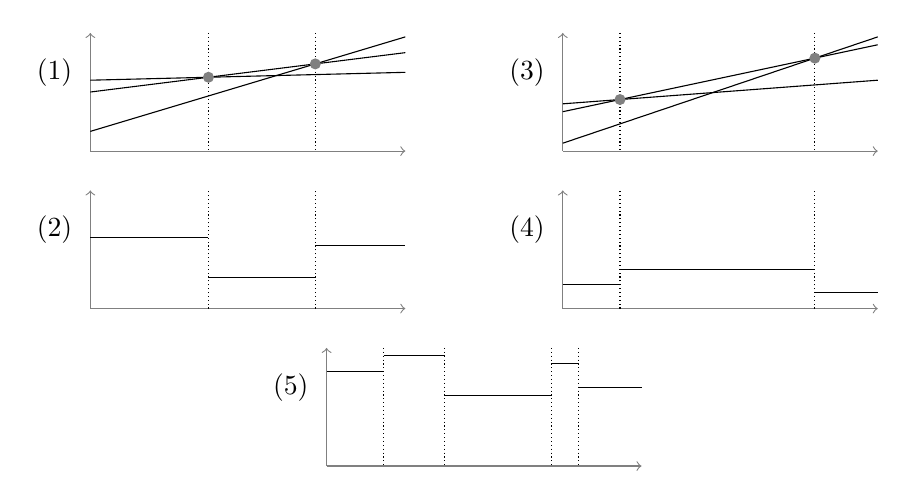
\begin{tikzpicture}
	\tikzstyle{axes} = [->,gray,thin]
	\tikzstyle{boundary} = [thin,densely dotted]

	% step 1
	\node [anchor=east,left=3pt] at (0,1) {(1)};
	\draw[axes] (0,0) -- +(0,1.5);
	\draw[axes] (0,0) -- +(4,0);
	\draw (0,0.25) node (a 1){} -- (4,1.45) node (b 1){};
	\draw (0,0.75) node (a 2){} -- (4,1.25) node (b 2){};
	\draw (0,0.9)node (a 3){} -- (4,1) node (b 3){};

	\path (intersection of a 1--b 1 and a 2--b 2) coordinate (bound 1);
	\draw[boundary] (bound 1 |- 0,1.5) -- (bound 1 |- 0,0);

	\path (intersection of a 3--b 3 and a 2--b 2) coordinate (bound 2);
	\draw[boundary] (bound 2 |- 0,1.5) -- (bound 2 |- 0,0);
	
	\fill[gray] (bound 1) circle (2pt);
	\fill[gray] (bound 2) circle (2pt);

	% step 2
	\node [anchor=east,left=3pt] at (0,-1) {(2)};
	\draw[axes] (0,-2) -- +(0,1.5);
	\draw[axes] (0,-2) -- +(4,0);

	\draw[boundary] (bound 1 |- 0,-2) -- (bound 1 |- 0,-0.5);
	\draw[boundary] (bound 2 |- 0,-2) -- (bound 2 |- 0,-0.5);

	\draw (0,-1.1) -- (0,-1.1 -| bound 2);
	\draw (4,-1.2 -| bound 1) -- (4, -1.2);
	\draw (bound 2 |- 0,-1.6) -- (bound 1 |- 0,-1.6);
	
	% step 3
	\node [anchor=east,left=3pt] at (6,1) {(3)};
	\draw[axes] (6,0) -- +(0,1.5);
	\draw[axes] (6,0) -- +(4,0);
	\draw (6,0.1) node (a 4){} -- (10,1.45) node (b 4){};
	\draw (6,0.5) node (a 5){} -- (10,1.35) node (b 5){};
	\draw (6,0.6) node (a 6){} -- (10,0.9) node (b 6){};

	\path (intersection of a 4--b 4 and a 5--b 5) coordinate (bound 3);
	\draw[boundary] (bound 3 |- 0,1.5) -- (bound 3 |- 0,0);

	\path (intersection of a 6--b 6 and a 5--b 5) coordinate (bound 4);
	\draw[boundary] (bound 4 |- 0,1.5) -- (bound 4 |- 0,0);
	
	\fill[gray] (bound 3) circle (2pt);
	\fill[gray] (bound 4) circle (2pt);


	% step 4
	\node [anchor=east,left=3pt] at (6,-1) {(4)};
	\draw[axes] (6,-2) -- +(0,1.5);
	\draw[axes] (6,-2) -- +(4,0);
	
	\draw[boundary] (bound 3 |- 0,-2) -- (bound 3 |- 0,-0.5);
	\draw[boundary] (bound 4 |- 0,-2) -- (bound 4 |- 0,-0.5);

	\draw (6,-1.7) -- (0,-1.7 -| bound 4);
	\draw (10,-1.8 -| bound 3) -- (10, -1.8);
	\draw (bound 4 |- 0,-1.5) -- (bound 3 |- 0,-1.5);

	% step 5
	\begin{scope}[xshift=3cm,yshift=-4cm]
		\node [anchor=east,left=3pt] at (0,1) {(5)};
		\draw[axes] (0,0) -- +(0,1.5);
		\draw[axes] (0,0) -- +(4,0);

		\path (0,0.25) node (a 1){} -- (4,1.45) node (b 1){};
		\path (0,0.75) node (a 2){} -- (4,1.25) node (b 2){};
		\path (0,0.9) node (a 3){} -- (4,1) node (b 3){};

		\path (intersection of a 1--b 1 and a 2--b 2) coordinate (bound 1);
		\draw[boundary] (bound 1 |- 0,1.5) -- (bound 1 |- 0,0);

		\path (intersection of a 3--b 3 and a 2--b 2) coordinate (bound 2);
		\draw[boundary] (bound 2 |- 0,1.5) -- (bound 2 |- 0,0);

		\path (0,0.1) node (a 4){} -- (4,1.45) node (b 4){};
		\path (0,0.5) node (a 5){} -- (4,1.35) node (b 5){};
		\path (0,0.6) node (a 6){} -- (4,0.9) node (b 6){};

		\path (intersection of a 4--b 4 and a 5--b 5) coordinate (bound 3);
		\draw[boundary] (bound 3 |- 0,1.5) -- (bound 3 |- 0,0);

		\path (intersection of a 6--b 6 and a 5--b 5) coordinate (bound 4);
		\draw[boundary] (bound 4 |- 0,1.5) -- (bound 4 |- 0,0);

		\draw (bound 2 |- 0,0.9) -- (bound 1 |- 0,0.9);
		\draw (bound 2 |- 0,1.4) -- (bound 4 |- 0,1.4);
		\draw (bound 1 |- 0,1.3) -- (bound 3 |- 0,1.3);

		\draw (0,1.2) -- (0,1.2 -| bound 4);
		\draw (4,1.0 -| bound 3) -- (4, 1.0);
	\end{scope}
	
\end{tikzpicture}
\end{center}}
\figpostamble
\caption[Illustration of the MERT line minimization algorithm.]{\label{fig:mer}Illustration of the MERT line minimization algorithm for optimizing a single parameter.  (1) For each candidate translation $\hat{\e}$, compute $P_{\lambda_k}(\hat{\e}|\f)$ as a function of $\lambda_k$, and
find the intervals at which the optimal candidate changes.  (2) Using these intervals, compute
$E_{\lambda_k}(\argmax_{\hat{\e}}P(\hat{\e}|\f),\e)$ as a function of $\lambda_k$.
(3) and (4) Repeat this procedure for each sentence.  (5) Add the single-sentence
error functions (2) and (4) to compute the aggregate error function 
for both input sentences.  To optimize, we simply walk along all intervals of the aggregate function
until we determine the minimum.}
\end{figure*}

\begin{equation}
\lambda_1^K = \argmin_{\hat{\lambda}_1^K} \sum_{(\e,\f)\in C}E(\argmax_{\hat{\e}} P_{\hat{\lambda}_1^K}(\hat{\e}|\f),\e)
\end{equation}


\algorithm{Minimum Error Rate Training}{
\begin{algorithmic}[1]
\State \textbf{Input} initial estimate $\lambda_{1,0}^K$ \Comment Uniform or random
\State \textbf{Input} training corpus $C$
\State $\lambda_1^K = \lambda_{1,0}^K$ 
\State $E_{best} = \sum_{(\e,\f) \in C}E(\argmax_{\hat{\e}}P_{\lambda_1^K}(\hat{\e}|\f),\e)$ \Comment Decode
\Repeat
  \State Generate $M$ random estimates $\lambda_{1,1}^K,...,\lambda_{1,M}^K$ \Comment To avoid poor local maximum
  \For {$m=\{0,1,...,M\}$}
    \For {$k=\{1,2,...,K\}$}
      \State $\lambda'_{k,m} =$ \Call{line-minimize}{$k, \lambda_{1,m}^K, C$}
      \State $E_{k,m} = \sum_{(\e,\f) \in C}E(\argmax_{\hat{\e}}P_{\lambda_{1,m}^{k-1}\lambda'_{k,m}\lambda_{k+1,m}^K}(\hat{\e}|\f),\e)$ \Comment $N$-best list
      \If {$E_{k,m} < E_{best}$}
        \State $\lambda_1^K = \lambda_{1,m}^{k-1}\lambda'_{k,m}\lambda_{k+1,m}^K$
        \State $E_{best} = E_{k,m}$
      \EndIf
    \EndFor
  \EndFor
  \State $\lambda_{1,0}^K=\lambda_1^K$
  \State $E_{best} = \sum_{(\e,\f) \in C}E(\argmax_{\hat{\e}}P_{\lambda_1^K}(\hat{\e}|\f),\e)$ \Comment Decode
\Until {no change in $\lambda_{1}^K$}
\State \Return $\lambda_{1,0}^K$
\State
\Function{line-minimize}{$k, \lambda_1^K, C$}
\State $E_{\lambda_k}(C) = 0$
\ForAll {$(\e,\f) \in C$}
  \ForAll {$\hat{\e} \in$ \Call{Decoder-N-Best}{$\f$}}
    \State $m_{\hat{\e}} = h_k(\hat{\e},\f)$  \Comment{slope of $P_{\lambda_k}(\hat{\e},\f)$}
    \State $b_{\hat{\e}} = \sum_{k'=1}^{k-1} \lambda_{k'}\cdot h_{k'}(\hat{\e},\f) + \sum_{k'=k+1}^{K} \lambda_{k'}\cdot h_{k'}(\hat{\e},\f)$  \Comment{intercept of $P_{\lambda_k}(\hat{\e},\f)$}
  \EndFor
  \State $i=0$
  \State $\Delta[i]= -\infty$ \Comment{left interval boundary}
  \State $e[i] = \argmin_{\hat{e}} m_{\hat{\e}}$ \Comment{equivalent to $\argmax_{\hat{\e}}\lim_{\lambda_k \rightarrow -\infty}P(\hat{\e},\f)$}
  \Repeat
    \State $i = i+1$
    \State $\Delta[i] =\min_{\hat{\e}}$ \Call{x-intersect}{$m_{\hat{e}},m_{e[i-1]},b_{\hat{e}},b_{e[i-1]}$} $ > \Delta[i-1]$
    \State $e[i] =\argmin_{\hat{\e}}$ \Call{x-intersect}{$m_{\hat{e}},m_{e[i-1]},b_{\hat{e}},b_{e[i-1]}$} $ > \Delta[i-1]$
  \Until {No more intersection points found}
  \State $\Delta_{i+1} = \infty$
  \State $E_{\lambda_k}(\argmax_{\hat{\e}}P(\hat{\e}|\f),\e) = \{ \lambda_k \rightarrow E(\hat{\e},\e) : \hat{\e} = e[i], \Delta[i] \leq \lambda_k \leq \Delta_{i+1}\}$
  \State $E_{\lambda_k}(C) += E_{\lambda_k}(\argmax_{\hat{\e}}P(\hat{\e}|\f),\e)$
\EndFor
\State \Return $\lambda_k = \argmin E_{\lambda_k}(C)$
\EndFunction
\end{algorithmic}
}

\noindent The optimization contains an
argmax operator, which precludes calculation
of a gradient.  Although there is
no way to find a guaranteed optimal solution
under these circumstances, we can find
a good solution using the method 
sketched in \citet{Och:2003:acl}, which
we describe in greater detail here due to its 
widespread use.
Pseudocode appears in Algorithm 1.

The MERT algorithm works by iteratively generating
random values for $\lambda_1^K$, which
it then tries to improve by minimizing each parameter
$\lambda_k$ in turn while holding the others constant. At the end of 
this optimization step, the optimized $\lambda_1^K$ yielding
the greatest error reduction is used as input
to the next iteration.

The single-parameter line minimization algorithm at the core of MERT 
is illustrated in \figureref{mer}.  It
is based on the observation that if we hold all but 
one parameter $\lambda_k$ constant, then $\Pef$ 
for any given pair $\e$ and $\f$ is $\Pef = \lambda_k h_k(\e,\f) + 
(\sum_{k'\neq k}\lambda_{k',m}h_{k'}(\e,\f))$.  
Note that the second term of the sum is constant,
making the function linear in $\lambda_k$.
Using the intersections of
these lines for all candidate translations
in a decoder's $N$-best list for a
single input sentence, the algorithm
exhaustively computes a representation of the
piecewise linear function $E(\argmax_{\hat{\e}} P(\hat{\e}|\f),\e))$.
Assuming that our error function is 
additive, we simply sum over all input
$(\e,\f)\in C$ to compute the complete function
that we are trying to  minimize.\footnote{Sometimes
this function is not additive, as is
the case with the commonly used BLEU score \citep{Papineni:2002:acl}.
Usually, however, the function is computed in terms of aggregate values
over the training set
which are additive.  If this is the case, we simply keep track of all
of the additive values which are used to compute the error function over
each interval, and then perform the computation once all intervals are 
known.}
We then select the midpoint in the interval which minimizes the 
function.

\figpreamble
\begin{figure*}[t]
\figfontsize{\begin{center}
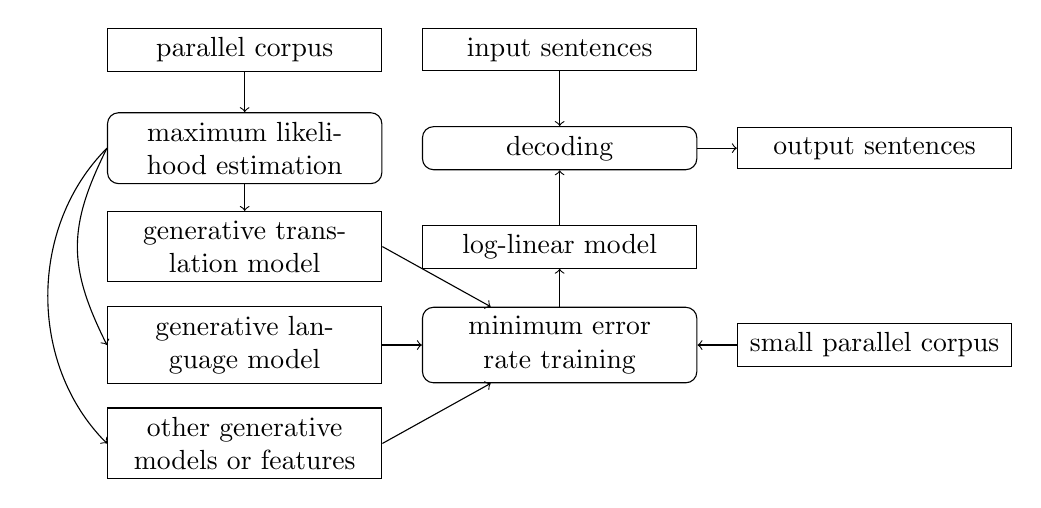
\begin{tikzpicture}[node distance=1.25cm]
	\tikzstyle{flow} = [text centered,text width=3.25cm]
	\tikzstyle{data} = [draw,rectangle,flow]
	\tikzstyle{process} = [draw,rectangle,rounded corners,flow]
	\node (corpus) [data] {parallel corpus};
	\node (mle) [process,below of=corpus] {maximum likelihood estimation};
	\node (tm) [data,below of=mle] {generative translation model};
	\node (lm) [data,below of=tm] {generative language model};
	\node (features) [data,below of=lm] {other generative models or features};
	\node (mert) [process,right of=lm,node distance=4cm] {minimum error rate training};
	\node (discriminative) [data,above of=mert] {log-linear model};
	\node (decoding) [process,above of=discriminative] {decoding};
	\node (input) [data,above of=decoding] {input sentences};
	\node (output) [data,right of=decoding,node distance=4cm] {output sentences};
	\node (dev) [data,right of=mert,node distance=4cm] {small parallel corpus};
	
	\draw[->] (corpus) -- (mle);
	\draw[->] (mle) -- (tm);
	\draw[->] (mle.west) .. controls +(-0.5,-1) and +(-0.5,1) .. (lm.west);
	\draw[->] (mle.west) .. controls +(-1,-1) and +(-1,1) .. (features.west);
	\draw[->] (tm.east) -- (mert);
	\draw[->] (lm.east) -- (mert.west);
	\draw[->] (features.east) -- (mert);
	\draw[->] (mert) -- (discriminative);
	\draw[->] (discriminative) -- (decoding);
	\draw[->] (input) -- (decoding);
	\draw[->] (dev) -- (mert);
	\draw[->] (decoding) -- (output);
\end{tikzpicture}
\end{center}}
\figpostamble
\caption{\label{fig:overview}The flow of data, models, and processes commonly involved in the deployment of an SMT system.}
\end{figure*}



\subsubsection{Purely Discriminative Training}\label{sec:pure-discriminative}

Most current state-of-the-art SMT systems use log-linear models
with a small number of generative submodels and use MERT in order 
to optimize whatever error function is chosen for evaluation.  
An overview of the architecture used in these systems is 
shown in \figureref{overview}.  This approach is not {\em purely}
discriminative; it uses generative model estimates as input
to a discriminative learner that optimizes a small number of 
feature weights.  In pure discriminative learning, 
features are usually binary or integral.  For instance, we might
define a word pair feature $h(e,f)$ as follows:

\begin{displaymath}
h(e,f) = \left\{\begin{array}{l}
1~{\rm if~the~input~contains~}f{\rm~and~the~output~contains}~e\\
0~{\rm otherwise}
\end{array}\right.
\end{displaymath}


\noindent Under this definition, the weight given
to this feature by the combined generative and discriminative 
training procedure outlined above is $\lambda\log p(f|e)$.  However,
as we have noted, $p(f|e)$ is estimated to maximize likelihood,
not translation performance.  We might instead wish to assign
a weight to this feature that is estimated to directly optimize
translation performance.  This is the goal of pure discriminative
learning, which can be accomplished by a number of different
algorithms.  Examples include the perceptron 
algorithm \citep{Liang:2006:acl-coling}, large margin learning
\citep{Tillman:2006:acl-coling,Watanabe:2007:emnlp-conll}, decision tree learning
\citep{Wellington:2006:amta}, and transductive learning 
\citep{Ueffing:2007:acl}.  Pure discriminative
learning is promising, but there are still a number of significant
obstacles to overcome, most notably the ability to scale to
the very large datasets and billions of parameters required for SMT.  The
present approaches are quite slow compared to generative model estimation
and MERT.


\section{Decoding}\label{sec:decoding}

Now that we have a model and estimates for all of our parameters, 
we can translate new input sentences.  This is called decoding.  
In principle, decoding corresponds solving the maximization problem
in Equation~\ref{eq:maximization}.

\begin{equation}\label{eq:maximization}
\evar = \argmax_{(\hat{\evar}:Y(\hat{\evar},\dvar))} P(\hat{\e},\dvar|\f)
\end{equation}

\noindent We call this the \term{decision rule}.  Equation~\ref{eq:maximization}
is not the only possible decision rule, although it is by far
the most common. Alternative decision rules are presented in
\citet{Kumar:2004:hlt} and \citet{Venugopal:2005:wpt}.

This is a difficult optimization.
Recall that $\Pedf$ ranges over $\{E^* \times D^* \times F^*\}$.  Even
though $\fvar$ is fixed, and even though the number of
possible outputs $(\evar,\dvar)$ is finite due to the 
constraints of our translational equivalence model,
there is still a very large number of them to
consider in order to maximize the function.
Therefore, a primary objective of decoding is
to search this space as efficiently as possible.

There are two types of decoders, corresponding to 
our two broad types of translational equivalence
models: FST and SCFG.

\subsection{FST Decoding}\label{sec:finite-state-decoding}

Nearly all approaches to finite-state decoding follow
a general framework described by \citet{Wang:1997:acl} and
\citep{Koehn:2004:amta}.  It is a generalization of speech
recognition algorithms originating in information 
theory \citet{Jelinek:1969:tr}.

In this algorithm, search proceeds through a directed
acyclic graph of 
states representing partial or completed translation
hypotheses, which are constructed from left-to-right in 
the target language word order.  An example graph
is depicted in \figureref{fst-search}.
Each state consists of the following elements.

\begin{asparaenum}
\item A coverage set $C \subseteq \{1,2,...,J\}$
enumerates the positions of the source
string $f_1^J$ that have been translated.
\item If using an $n$-gram language model,
the $n-1$ most recently generated target words 
are kept for computing the $n$-gram
language model component of the probability.
These words and the subset $C$ constitute the
state's signature.
\item The cost $h$ of our partial hypothesis is computed as
the combination of model costs associated with the hypothesis.
This will be fairly straightforward for any generative 
model based on the underlying translational equivalence
model, since we will be reconstructing the events that 
occur in that model, and we can simply apply the 
associated probabilities.  It may or may not be difficult
for a discriminative model, depending on the specific
feature functions.
\item The estimated cost $g$ of completing the partial hypothesis
is computed heuristically.  Because this computation must be
done quickly, we usually use only the single-best
word-to-word (or phrase-to-phrase) costs in this 
heuristic function \citep{Koehn:2004:amta}.
\end{asparaenum}

\figpreamble
\begin{figure*}[t]
\figfontsize{\begin{center}
\begin{tikzpicture}
	\tikzstyle{state} = [draw,fill=white]
	\tikzstyle{uncovered} = [scale=0.4,circle,draw]
	\tikzstyle{covered} = [uncovered,fill=black]
	\tikzstyle{word 1} = [uncovered]
	\tikzstyle{word 2} = [uncovered]
	\tikzstyle{word 3} = [uncovered]
	\tikzstyle{word 4} = [uncovered]
	\tikzstyle{word 5} = [uncovered]
	\tikzstyle{word 6} = [uncovered]
	\tikzstyle{word 7} = [uncovered]
	\tikzstyle{word 8} = [uncovered]
	\tikzstyle{word 9} = [uncovered]
	\tikzstyle{word 10} = [uncovered]
	\tikzstyle{word 11} = [uncovered]

	\newcommand{\searchitem}[3]{
		\matrix (#1) [state,anchor=south,above=3pt] at (#3) {
			\node[minimum height=12pt]{#2}; \\
			\node (center) [word 6] {}; 
			\node (cover) [anchor=west,word 7] at (center.east) {}; 
			\node (cover) [anchor=west,word 8] at (cover.east) {}; 
			\node (cover) [anchor=west,word 9] at (cover.east) {}; 
			\node (cover) [anchor=west,word 10] at (cover.east) {}; 
			\node (cover) [anchor=west,word 11] at (cover.east) {}; 
			\node (cover) [anchor=east,word 5] at (center.west) {}; 
			\node (cover) [anchor=east,word 4] at (cover.west) {}; 
			\node (cover) [anchor=east,word 3] at (cover.west) {}; 
			\node (cover) [anchor=east,word 2] at (cover.west) {}; 
			\node (cover) [anchor=east,word 1] at (cover.west) {}; \\
		};
	}

	\path (0,0) coordinate (stack 1);
	\path (4.5,0) coordinate (stack 2);
	\path (9,0) coordinate (stack 3);

	\node [anchor=south,rectangle,minimum height=5.5cm,minimum width=2.25cm,fill=lightgray] at (stack 1) {};
	\node [anchor=south,rectangle,minimum height=5.5cm,minimum width=2.25cm,fill=lightgray] at (stack 2) {};
	\node [anchor=south,rectangle,minimum height=5.5cm,minimum width=2.25cm,fill=lightgray] at (stack 3) {};


	\searchitem{start}{$\varepsilon$}{stack 1}

	\tikzstyle{word 1} = [covered]
	\searchitem{item 1}{Although}{stack 2}
	\searchitem{item 2}{However}{item 1.north}

	\tikzstyle{word 1} = [uncovered]
	\tikzstyle{word 7} = [covered]
	\searchitem{item 3}{sky}{item 2.north}
	
	\tikzstyle{word 7} = [uncovered]
	\tikzstyle{word 1} = [covered]
	\tikzstyle{word 2} = [covered]
	\searchitem{item 4}{north}{stack 3}
	\searchitem{item 5}{northern}{item 4.north}

	\tikzstyle{word 7} = [covered]
	\tikzstyle{word 1} = [uncovered]
	\searchitem{item 6}{north}{item 5.north}

	\tikzstyle{word 2} = [uncovered]
	\tikzstyle{word 8} = [covered]
	\searchitem{item 7}{remained}{item 6.north}

	\tikzstyle{word 7} = [uncovered]
	\tikzstyle{word 8} = [uncovered]
	\tikzstyle{word 2} = [covered]
	\tikzstyle{word 3} = [covered]
	\searchitem{item 8}{wind}{item 7.north}


	
	\draw[->] (start.east) -- (start.east -| item 1.west) node [pos=0.6,above] {1: Although};
	\draw[->] (start.east) ..controls +(1,0.5) and +(-3,0) .. (item 2.west) node [pos=0.8,above] {1: However};
	\draw[->] (start.east) ..controls +(1,1) and +(-3,0) .. (item 3.west) node [pos=0.8,above] {7: sky};
	\draw[->] (item 1.east) -- (item 1.east -| item 4.west) node [pos=0.5,below] {2: north};
	\draw[->] (item 1.east) ..controls +(1,0.5) and +(-3,0) .. (item 2.east -| item 5.west) node [pos=0.85,below] {2: northern};
	\draw[->] (item 2.east) ..controls +(1,-0.5) and +(-3,0) .. (item 1.east -| item 4.west) node [pos=0.85,above] {2: north};
	\draw[->] (item 2.east) -- (item 2.east -| item 5.west) node [pos=0.5,above] {2: northern};
	\draw[->] (item 3.east) -- (item 3.east -| item 6.west) node [pos=0.5,above] {2: north};
	\draw[->] (item 3.east) ..controls +(1,0.5) and +(-3,0) .. (item 7.west) node [pos=0.8,above] {8: remained};
	\draw[->] (start) ..controls +(1,3) and +(-6,0) .. (item 8.west) node [pos=0.9,above] {2--3: north wind};

	\draw[->] (item 4.east) -- +(0.5,0.25);
	\draw[->] (item 4.east) -- +(0.5,0);
	\draw[->] (item 4.east) -- +(0.5,-0.25);
	\draw[->] (item 5.east) -- +(0.5,0.25);
	\draw[->] (item 5.east) -- +(0.5,0);
	\draw[->] (item 5.east) -- +(0.5,-0.25);
	\draw[->] (item 6.east) -- +(0.5,0.25);
	\draw[->] (item 6.east) -- +(0.5,0);
	\draw[->] (item 6.east) -- +(0.5,-0.25);
	\draw[->] (item 7.east) -- +(0.5,0.25);
	\draw[->] (item 7.east) -- +(0.5,0);
	\draw[->] (item 7.east) -- +(0.5,-0.25);
	\draw[->] (item 8.east) -- +(0.5,0.25);
	\draw[->] (item 8.east) -- +(0.5,0);
	\draw[->] (item 8.east) -- +(0.5,-0.25);

	\matrix (chinese sentence) [nodes={anchor=mid},above of=item 3,node distance=4.5cm] {
		\node{\zh{虽然}}; & 
		\node{\zh{北}}; & 
		\node{\zh{风}}; & 
		\node{\zh{呼啸}}; & 
		\node{\zh{,}}; & 
		\node{\zh{但}}; & 
		\node{\zh{天空}}; & 
		\node{\zh{依然}}; & 
		\node{\zh{十分}}; & 
		\node{\zh{清澈}}; & 
		\node{~~\zh{。}}; \\
		\node{\em Although}; & 
		\node{\em north}; & 
		\node{\em wind}; & 
		\node{\em howls}; & 
		\node{\em ,}; & 
		\node{\em but}; & 
		\node{\em sky}; & 
		\node{\em still}; & 
		\node{\em extremely}; & 
		\node{\em limpid}; & 
		\node{\em .~}; \\
		\node{1}; & 
		\node{2}; &
		\node{3}; &
		\node{4}; &
		\node{5}; &
		\node{6}; &
		\node{7}; &
		\node{8}; &
		\node{9}; & 
		\node{10}; &
		\node{11}; \\
	};
	
	\node (label 2) [anchor=south east,left=5mm] at (start.west) {(2)};
	\node (label 1) [above of=label 2,node distance=6cm] {(1)};
	
\end{tikzpicture}
\end{center}}
\figpostamble
\caption[Illustration of search in a finite-state decoder]{Illustration of search in a finite-state decoder.  The input
sentence (1) generates a large search graph, partially illustrated
in (2).  In this illustration, each arrow represents extension of a
hypothesis by appending the words on the arrow.  To recover the best 
translation, we traverse the highest scoring path.  In each state, we
show the coverage set and most recently generated target word,
which is needed for computation of a bigram language model.  
Note that states can only be combined if
the coverage set and the most recently produced words match.  Items with
the same number of covered words are stored in the same stack.}
\label{fig:fst-search}
\end{figure*}

Hypotheses in this space are extended 
by adding one or more source word indices to the coverage set
and appending one or more target words to the 
hypothesis string to produce a new state.  This corresponds
to the translation of the newly covered source words by
the newly generated target words.  We apply model
probabilities accordingly to update the partial cost $h$.
We implement model-specific extension
operators to apply this algorithm to IBM Model~4 
\citep{Tillman:2003:cl,Germann:2004:ai},
phrase-based models \citep{Koehn:2004:amta}, or any number of other
finite-state translation models 
\citep{Wang:1997:acl,Niessen:1998:acl}.  

In order to organize the search space, hypotheses may be
stored in one or more priority queues, usually corresponding
to either the cardinality $|C|$ of the coverage set,
or to the coverage sets themselves \citep{Tillman:2003:cl}.\footnote{This priority
queue is often called a \term{stack} in literature, and the 
algorithm that we describe is called \term{stack decoding},
although its central object is technically not a stack.
The terminology dates back to \citet{Jelinek:1969:tr}.}
This is done to ensure that comparisons between
hypotheses---used for sorting and pruning purposes within
each priority queue---
are done on hypotheses of relatively equal depth in the search
space.~\citep{Wang:1997:acl}  If we were to compare hypotheses
of unequal length, our heuristic functions, which favor
shorter hypotheses, will cause more complete hypotheses
to be pruned from the priority queue prior to full
evaluation.  

Each hypothesis contains a backpointer to the hypothesis that generated
it.  If two hypotheses have matching signatures, only the 
higher-scoring hypothesis is kept \citep{Och:2001:ddmmt,Koehn:2004:amta}.  
This is a risk-free optimization because the set of all extensions
to these two hypotheses will be the same; therefore the higher-scoring
partial hypothesis is guaranteed to generate a higher-scoring completed 
hypothesis.

The search space defines a finite-state 
word lattice, in which we can 
find the score of any particular hypothesis by 
traversing the lattice~\citep{Ueffing:2002:emnlp,Koehn:2004:amta}.  We can
use standard finite-state methods for finding the 
best path (or paths) through this lattice.  It is possible
to directly implement such decoders as a cascade
of weighted finite-state transducers 
\citep{Knight:1998:amta,Kumar:2006:nle}.  These
transducers will differ from the ones we describe
in \sectionref{finite-state-models}.  However, 
the decoding algorithm we have described does, in
principle, reverse the set of transductions 
represented by those models; we can see, for instance,
that it reconstructs the English sentence in the order
that it was fed into the transducer, at 
each step consuming the source words that were 
created by transductions over the associated 
target word or words.

A variant algorithm allows the target language
hypothesis to be extended to either left or right
\citep{Watanabe:2002:coling}.


\subsubsection{Optimality and Pruning}\label{sec:optimality-and-pruning}
Using $A^*$ heuristics, we can solve the optimization in 
Equation~\ref{eq:maximization} exactly \citep{Och:2001:ddmmt}.
\citet{Germann:2004:ai} illustrate
how we can also do this by converting the problem to a linear integer
programming problem and using standard tools to solve it.  Due to
the large number of translations for each word or phrase, 
even with limited reordering this can be very slow.
Fortunately, optimal search is not strictly necessary,
because there are many good translations of 
any sentence.  If many of these receive high probability under
our model, then we may safely permit a certain amount of \term{search error}.
Search error occurs when the decoder does not choose the globally highest-scoring
hypothesis according to the model, but rather some other high-scoring
hypothesis that can be found more quickly.  We can optimize for speed
by {\em pruning} the search graph \citep{Tillman:2003:cl,Koehn:2004:amta}.
In {\em threshold pruning}, any hypothesis
with a probability less than $t$ times the probability of the 
best estimate in the same priority queue is removed.  In {\em histogram
pruning}, only the $n$ best hypotheses are kept in any priority queue.
Search with pruning is sometimes called \term{beam search},
where $t$ or $n$ is the size of the {\em beam}.
With a well-tuned beam size, we 
gain large speedups with very little loss of accuracy
\citep{Tillman:2003:cl,Zens:2004:hlt-naacl,Koehn:2004:amta,Germann:2004:ai}.


\subsubsection{Greedy Decoding}\label{sec:greedy-decoding}
An alternative to standard finite-state decoding is 
greedy decoding \citep{Marcu:2002:emnlp,Germann:2003:naacl,Germann:2004:ai}.
In greedy decoding, we generate an initial hypothesis
by substituting each source word with the 
highest-probability target word, using the
original target word order.  This gives us a complete word-for-word
gloss of the source sentence.  We then use hill-climbing 
heuristics in an attempt to find higher-scoring hypotheses
by considering neighboring translations produced by
changing the order or translation of one or two words
at a time, and choosing the highest-scoring neighbor.
This new hypothesis becomes the starting point for
the next iteration of the algorithm. 
The algorithm terminates when 
no higher-scoring hypothesis can
be found.  With some optimizations, it algorithm runs
in time nearly linear in target sentence length 
\citep{Germann:2003:naacl}.  A tradeoff of 
is that the search error rate is 
much higher than stack decoding \citep{Germann:2004:ai}.



\subsection{SCFG Decoding}\label{sec:syntax-based-decoding}

Decoding with SCFG models is equivalent
to CFG parsing \citep{Melamed:2004:acl:smtbyp}.
The goal is to infer the highest-scoring tree that
generates the input sentence using the source side of the
grammar, and then read off the tree in target order.
Most practical SCFG decoders are straightforward 
extensions of dynamic programming algorithms
for parsing monolingual context-free grammars 
\citep{Wu:1998:acl,Yamada:2002:acl,Zens:2003:acl,Chiang:2007:cl,Marcu:2006:emnlp,Venugopal:2007:hlt-naacl}.  
A benefit of this is that the standard algorithms and 
optimizations that have been developed for CFG
parsing can be applied to SMT 
\citep{Melamed:2004:acl:smtbyp}.

SCFG decoding works by attempting to cover larger
and larger \term{spans} of the input sentence.  A span
is simply a contiguous sequence of words. States
in the search space consist of a span, a nonterminal
symbol which covers the span, and any language model
information needed to combine spans 
\citep{Melamed:2004:tmi,Chiang:2007:cl,Zhang:2006:hlt-naacl}.  In order to 
construct larger spans, we find SCFG productions whose
right-hand sides match a sequence of nonterminals that
we have already inferred to cover a set of smaller, adjacent spans.  Once
we have constructed the full source language parse,
we produce output using an in-order traversal based
on target language ordering of the tree.  This is illustrated in 
\figureref{cky}.

\figpreamble
\begin{figure*}[t]
\figfontsize{\begin{center}
\begin{tikzpicture}[node distance=2cm]

	\matrix (words) [column sep=3cm,matrix of nodes]{
		|(word 2)| \zh{北} & 
		|(word 3)| \zh{风} & 
		|(word 4)| \zh{呼啸} \\
		{\em north} &
		{\em wind} &
		{\em howls} \\
		2 &
		3 &
		4 \\
	};


	\matrix (item 1)[draw,matrix of nodes,above of=word 2]{
		& |[minimum width=8mm]| JJ & \\
		1 & & 2 \\
	};
	\draw (item 1-1-2.south) -- (item 1-2-1.east) -- (item 1-2-3.west) -- cycle;

	\matrix (item 2)[draw,matrix of nodes,above of=word 3]{
		& |[minimum width=8mm]| NN & \\
		2 & & 3 \\
	};
	\draw (item 2-1-2.south) -- (item 2-2-1.east) -- (item 2-2-3.west) -- cycle;

	\matrix (item 3)[draw,matrix of nodes,above of=word 4]{
		& |[minimum width=8mm]| JJ & \\
		3 & & 4 \\
	};
	\draw (item 3-1-2.south) -- (item 3-2-1.east) -- (item 3-2-3.west) -- cycle;

	\draw[->] (word 2) -- (item 1) node [pos=0.5,fill=white] {JJ $\longrightarrow $ \zh{北}~/~north};
	\draw[->] (word 3) -- (item 2) node [pos=0.5,fill=white] {NN $\longrightarrow $ \zh{风}~/~wind};
	\draw[->] (word 4) -- (item 3) node [pos=0.5,fill=white] {JJ $\longrightarrow $ \zh{呼啸}~/~strong};

	\path (item 1.north) -- (item 2.north) coordinate[pos=0.5] (item 1 2);
	\path (item 1 2) -- +(0,1.5) coordinate (item 4 pos);

	\matrix (item 4)[draw,matrix of nodes,anchor=south] at (item 4 pos){
		& |[minimum width=8mm]| NPB & \\
		1 & & 3 \\
	};
	\draw (item 4-1-2.south) -- (item 4-2-1.east) -- (item 4-2-3.west) -- cycle;
	
	\draw[->,rounded corners] (item 1.north) -- +(0,0.25) coordinate (knee) -- (knee -| item 4 pos) -- (item 4.south);
	\draw[->,rounded corners] (item 2.north) -- +(0,0.25) coordinate (knee) -- (knee -| item 4 pos) -- (item 4.south) node [pos=0.5,fill=white] {$\NPB \longrightarrow  \cidx{\JJ}{1}\cidx{\NN}{2} ~/~ \cidx{\JJ}{1}\cidx{\NN}{2}$};


	\path (item 4.north) -- (item 4.north -| item 3.north) coordinate[pos=0.5] (item 3 4);
	\path (item 3 4) -- +(0,1.5) coordinate (item 5 pos);
	
	\matrix (item 5)[draw,matrix of nodes,anchor=south] at (item 5 pos){
		& |[minimum width=8mm]| NPB & \\
		1 & & 4 \\
	};
	\draw (item 5-1-2.south) -- (item 5-2-1.east) -- (item 5-2-3.west) -- cycle;

	\draw[->,rounded corners] (item 4.north) -- +(0,0.25) coordinate (knee) -- (knee -| item 5 pos) -- (item 5.south);
	\draw[->,rounded corners] (item 3.north) -- (item 3.north |- knee) -- (knee -| item 5 pos) -- (item 5.south) node [pos=0.5,fill=white] {$\NPB \longrightarrow  \cidx{\NPB}{1}\cidx{\JJ}{2} ~/~ \cidx{\JJ}{2}\cidx{\NPB}{1}$};

	\matrix (item 6)[draw,matrix of nodes,left of=item 5,node distance=3cm] {
		& |[minimum width=8mm]| DT & \\
		1 & & 1 \\
	};
	\draw (item 6-1-2.south) -- (item 6-2-1.east) -- (item 6-2-3.west) -- cycle;

	\draw[<-|,rounded corners] (item 6.south) -- +(0,-1) -- +(-3,-1) node[pos=0.5,above] {$\DT \longrightarrow  \textrm{the} ~/~ \varepsilon$};

	\path (item 5.north) -- (item 6.north) coordinate [pos=0.5] (item 5 6);
	\path (item 5 6) -- +(0,1.5) coordinate (item 7 pos);

	\matrix (item 7)[draw,matrix of nodes,anchor=south] at (item 7 pos) {
		& |[minimum width=8mm]| NP & \\
		1 & & 4 \\
	};
	\draw (item 7-1-2.south) -- (item 7-2-1.east) -- (item 7-2-3.west) -- cycle;
	
	\draw[->,rounded corners] (item 5.north) -- +(0,0.25) coordinate (knee) -- (knee -| item 7 pos) -- (item 7.south);
	\draw[->,rounded corners] (item 6.north) -- (item 6.north |- knee) -- (knee -| item 7 pos) -- (item 7.south) node [pos=0.5,fill=white] {$\NP  \longrightarrow  \cidx{\DT}{1}\cidx{\NPB}{2} ~/~ \cidx{\DT}{1}\cidx{\NPB}{2}$};


	\tikzstyle{every child} = [level distance=1cm]
	\tikzstyle{edge from parent} = [draw,->]
	\node (cfg) [right of=item 7,node distance=4.5cm] {NP} 
		child {node {DT}{
			child {node {the}}
		}} 
		child {node {NPB} 
			child {node {JJ}{
				child {node {strong}}
			}} 
			child {node {NPB}{[sibling distance=1cm]
				child {node {JJ}{
					child {node {north}}
				}}
				child {node {NN}{
					child {node {wind}}
				}}
			}
		} 
	}; 
	
	\draw[->,gray,densely dotted] (item 7) -- (cfg);

	\node (label 1) [anchor=east,left=5mm] at (words.west) {(1)};
	\node (label 2) at (label 1 |- item 1) {(2)};
	\node (label 3) at (label 1 |- item 4) {(3)};
	\node (label 4) at (label 1 |- item 6) {(4)};
	\node (label 5) at (label 1 |- item 7) {(5)};


\end{tikzpicture}
\end{center}}
\figpostamble
\caption[Illustration of SCFG decoding.]{Illustration of SCFG decoding.
(1) Scan each source word and associate it with a span. 
(2) Apply SCFG rules that match the target spans.
(3) Recursively infer larger spans from smaller spans. 
(4) Optionally infer any target language words with no
matching span in the source language.
(5) Read off the tree in target-language order.}
\label{fig:cky}
\end{figure*}

There are $O(J^2)$ possible spans in the source sentence,
and they can be computed in polynomial time.  
It is easy to see from this that SCFG decoding
is, {\em in principle}, much less computationally expensive
than FST decoding with full reordering.  However,
most practical FST decoders allow only a limited amount
of reordering, and in practice they are often much faster
than SCFG decoders.\footnote{It is possible to apply
reordering constraints of FST models to SCFG models.
\citet{Chiang:2005:acl,Chiang:2007:cl} restricts
hierarchical reordering to spans that are shorter than
ten words.  Spans longer than this are required to be
monotonic orderings of smaller
hierarchical phrases.  This prevents some long-distance
reordering.}  Search optimization for these models
is therefore an active area of research.

\citet{Chiang:2007:cl} describes a optimization
called {\em cube pruning} that prevents excessive combination
of hypotheses in adjacent subspans.  \citet{Zhang:2006:hlt-naacl}
describe a method for {\em binarizing} rules containing more
than two nonterminals, which helps reduce grammar constants for
parsing and simplifies $n$-gram language model integration.
\citet{Venugopal:2007:hlt-naacl} present a
method based on delayed language model integration, in which
the parse graph is first constructed quickly with simplified language
model statistics, and then expanded in a second pass using a full
language model, following only the most promising paths.  A number of
other optimizations have also been investigated
\citep{Huang:2005:iwpt:k-best,Huang:2007:acl}

\subsection{Reranking}\label{sec:reranking}

Even if there are no search errors and we produce the 
translation that exactly optimizes our decision rule, 
the translations produced by our decoder may not be 
the actual best translations according to human judgement.
It is possible that the search space explored by the decoder 
contained a better translation, and our decoder 
assigned a lower score for this hypothesis because its
estimate of $\Pedf$ was incorrect.
This is called \term{model error}.

One approach to reducing model error 
is \term{reranking} or \term{rescoring}.  In reranking, 
we first run our decoder, and rather than merely returning the 
highest-scoring translation, we return $N$ highest-scoring 
translations for some value $N$.
These translations are then input to an alternative model with 
access to more feature functions than may be efficiently computed in 
our decoder, or which are otherwise difficult to incorporate.
Hopefully, this alternative model can give us more
accurate scores than the one used in decoding.

Reranking approaches to SMT are described in 
\citet{Och:2004:naacl} and \citet{Shen:2004:naacl}.
\citet{Och:2004:naacl} show using oracle studies on
decoder $n$-best lists that large gains in accuracy are possible
with rescoring, although so far these are unrealized.

\section{Evaluation}\label{sec:evaluation}

How can we know if the output of our SMT system is any good?
Many methods have been proposed to evaluate MT output. 
\citet{Hovy:2002:mt} attribute to Yorick Wilks the remark that
``more has been written about MT evaluation over the past 50 
years than about MT itself''.
In the discussion that follows, we will narrowly focus on methods that
have figured prominently in the evaluation of statistical systems.

Traditionally accepted measures of MT evaluation have
required examination of MT system output by human
judges, who rank the \term{adequacy} of the translation
in conveying the source language meaning and the 
\term{fluency} of expression in the target language \citep{White:1994:amta}.
More ideal than this are measures which
determine how well some human task can be performed when
the human subject is provided with machine 
translated text.  If possible, we would optimize for 
task-related metrics directly.  
Unfortunately, human metrics require time and money.  
This usually rules out their use in 
iterative system development, where
we will need to perform regular evaluation to 
determine if changes are beneficial to performance.
The next best thing is to develop automatic
metrics that closely correlate with human 
evaluations.  The closer that these metrics are 
to the real objective, the better our performance
on that objective will be after we apply 
discriminative training (\sectionref{log-linear-estimation}).

A common element of automatic metrics is their use of a 
set of test sentences for which we already 
have human translations, called \term{reference translations}.
They can come from a parallel corpus, although we
must take care to use a separate set of sentences 
from the set we used for training.  The intuition
behind metrics based on reference sentences is
that MT must be good if it closely resembles human
translation of the same sentence \citep{Papineni:2002:acl}. 
These metrics are based on partial string 
matching between the output and
the reference translations, as illustrated
in \figureref{multi-evaluation}.  However, the use
of a single reference may bias the evaluation towards
a particular translation style.  In order to mitigate
against this and reflect the diversity of possible 
good translations, we may use multiple references.  This requires the use
of human translators to produce the additional
references, but it is a one-time cost.

\figpreamble
\begin{figure*}[t]
\figfontsize{\begin{center}
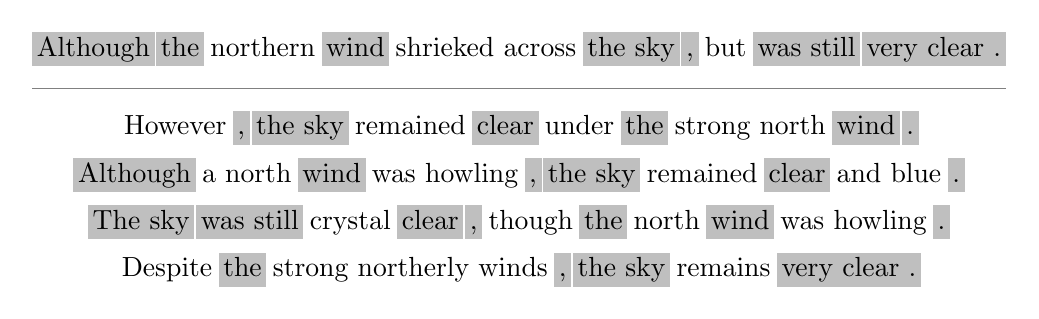
\begin{tikzpicture}[node distance=0.6cm]
	\tikzstyle{eval hilite}=[fill=lightgray]

	% hypothesis
	\matrix (sentence) [inner sep=0pt,column sep=1pt,nodes={inner sep=1.5pt,anchor=mid}]{
		\node (segment 0) {Although}; &
		\node (segment 1) {the}; &
		\node (segment 2) {northern}; &
		\node (segment 3) {wind}; &
		\node (segment 4) {shrieked across}; &
		\node (segment 5) {the sky}; &
		\node (segment 6) {,}; &
		\node (segment 7) {but}; &
		\node (segment 8) {was still}; &
		\node (segment 9) {very clear .}; \\
	};
	\path[eval hilite] 
		(segment 0.north west |- sentence.north west) rectangle (segment 0.south east |- sentence.south west);
	\path[eval hilite] 
		(segment 1.north west |- sentence.north west) rectangle (segment 1.south east |- sentence.south west);
	\path[eval hilite] 
		(segment 3.north west |- sentence.north west) rectangle (segment 3.south east |- sentence.south west);
	\path[eval hilite] 
		(segment 5.north west |- sentence.north west) rectangle (segment 5.south east |- sentence.south west);
	\path[eval hilite] 
		(segment 6.north west |- sentence.north west) rectangle (segment 6.south east |- sentence.south west);
	\path[eval hilite] 
		(segment 8.north west |- sentence.north west) rectangle (segment 8.south east |- sentence.south west);
	\path[eval hilite] 
		(segment 9.north west |- sentence.north west) rectangle (segment 9.south east |- sentence.south west);
	
	\node at (segment 0) {Although};
	\node at (segment 1) {the};
	\node at (segment 3) {wind};
	\node at (segment 5) {the sky};
	\node at (segment 6) {,};
	\node at (segment 8) {was still};
	\node at (segment 9) {very clear .};

	\path (sentence.west) -- +(0cm,-0.5cm) coordinate (separator start);
	\draw[thin,gray] (separator start) -- (separator start -| sentence.south east);

	% first reference sentence 
	\matrix (sentence) [inner sep=0pt,column sep=1pt,nodes={inner sep=1.5pt,anchor=mid},below of=sentence,node distance=1cm]{
		\node (segment 0) {However}; &
		\node (segment 1) {,}; &
		\node (segment 2) {the sky}; &
		\node (segment 3) {remained}; &
		\node (segment 4) {clear}; &
		\node (segment 5) {under}; &
		\node (segment 6) {the}; &
		\node (segment 7) {strong north}; &
		\node (segment 8) {wind}; &
		\node (segment 9) {.}; \\
	};
	\path[eval hilite] 
		(segment 1.north west |- sentence.north west) rectangle (segment 1.south east |- sentence.south west);
	\path[eval hilite] 
		(segment 2.north west |- sentence.north west) rectangle (segment 2.south east |- sentence.south west);
	\path[eval hilite] 
		(segment 4.north west |- sentence.north west) rectangle (segment 4.south east |- sentence.south west);
	\path[eval hilite] 
		(segment 6.north west |- sentence.north west) rectangle (segment 6.south east |- sentence.south west);
	\path[eval hilite] 
		(segment 8.north west |- sentence.north west) rectangle (segment 8.south east |- sentence.south west);
	\path[eval hilite] 
		(segment 9.north west |- sentence.north west) rectangle (segment 9.south east |- sentence.south west);
	\node at (segment 1) {,};
	\node at (segment 2) {the sky};
	\node at (segment 4) {clear};
	\node at (segment 6) {the};
	\node at (segment 8) {wind};
	\node at (segment 9) {.};

	% second reference sentence
	\matrix (sentence) [inner sep=0pt,column sep=1pt,nodes={inner sep=1.5pt,anchor=mid},below of=sentence]{
		\node (segment 0) {Although}; &
		\node (segment 1) {a north}; &
		\node (segment 2) {wind}; &
		\node (segment 3) {was howling}; &
		\node (segment 3 2) {,}; & % oops
		\node (segment 4) {the sky}; &
		\node (segment 5) {remained}; &
		\node (segment 6) {clear}; &
		\node (segment 7) {and blue}; &
		\node (segment 8) {.}; \\
	};
	\path[eval hilite] 
		(segment 0.north west |- sentence.north west) rectangle (segment 0.south east |- sentence.south west);
	\path[eval hilite] 
		(segment 2.north west |- sentence.north west) rectangle (segment 2.south east |- sentence.south west);
	\path[eval hilite] 
		(segment 4.north west |- sentence.north west) rectangle (segment 4.south east |- sentence.south west);
	\path[eval hilite] 
		(segment 6.north west |- sentence.north west) rectangle (segment 6.south east |- sentence.south west);
	\path[eval hilite] 
		(segment 8.north west |- sentence.north west) rectangle (segment 8.south east |- sentence.south west);
	\path[eval hilite] 
		(segment 3 2.north west |- sentence.north west) rectangle (segment 3 2.south east |- sentence.south west);
	\node at (segment 0) {Although};
	\node at (segment 2) {wind};
	\node at (segment 3 2) {,};
	\node at (segment 4) {the sky};
	\node at (segment 6) {clear};
	\node at (segment 8) {.};

	% third reference sentence
	\matrix (sentence) [inner sep=0pt,column sep=1pt,nodes={inner sep=1.5pt,anchor=mid},below of=sentence]{
		\node (segment 0) {The sky}; &
		\node (segment 1) {was still}; &
		\node (segment 2) {crystal}; &
		\node (segment 3) {clear}; &
		\node (segment 4) {,}; &
		\node (segment 5) {though}; &
		\node (segment 6) {the}; &
		\node (segment 7) {north}; &
		\node (segment 8) {wind}; &
		\node (segment 9) {was howling}; &
		\node (segment 10){.};\\
	};
	\path[eval hilite] 
		(segment 0.north west |- sentence.north west) rectangle (segment 0.south east |- sentence.south west);
	\path[eval hilite] 
		(segment 1.north west |- sentence.north west) rectangle (segment 1.south east |- sentence.south west);
	\path[eval hilite] 
		(segment 3.north west |- sentence.north west) rectangle (segment 3.south east |- sentence.south west);
	\path[eval hilite] 
		(segment 4.north west |- sentence.north west) rectangle (segment 4.south east |- sentence.south west);
	\path[eval hilite] 
		(segment 6.north west |- sentence.north west) rectangle (segment 6.south east |- sentence.south west);
	\path[eval hilite] 
		(segment 8.north west |- sentence.north west) rectangle (segment 8.south east |- sentence.south west);
	\path[eval hilite] 
		(segment 10.north west |- sentence.north west) rectangle (segment 10.south east |- sentence.south west);
	\node at (segment 0) {The sky};
	\node at (segment 1) {was still};
	\node at (segment 3) {clear};
	\node at (segment 4) {,};
	\node at (segment 6) {the};
	\node at (segment 8) {wind};
	\node at (segment 10) {.};

	% fourth reference sentence
	\matrix (sentence) [inner sep=0pt,column sep=1pt,nodes={inner sep=1.5pt,anchor=mid},below of=sentence]{
		\node (segment 0) {Despite}; &
		\node (segment 1) {the}; &
		\node (segment 2) {strong northerly winds}; &
		\node (segment 3) {,}; &
		\node (segment 4) {the sky}; &
		\node (segment 5) {remains}; &
		\node (segment 6) {very clear .}; \\
	};
	\path[eval hilite] 
		(segment 1.north west |- sentence.north west) rectangle (segment 1.south east |- sentence.south west);
	\path[eval hilite] 
		(segment 3.north west |- sentence.north west) rectangle (segment 3.south east |- sentence.south west);
	\path[eval hilite] 
		(segment 4.north west |- sentence.north west) rectangle (segment 4.south east |- sentence.south west);
	\path[eval hilite] 
		(segment 6.north west |- sentence.north west) rectangle (segment 6.south east |- sentence.south west);
	\node at (segment 1) {the};
	\node at (segment 3) {,};
	\node at (segment 4) {the sky};
	\node at (segment 6) {very clear .};



\end{tikzpicture}
\end{center}}
\figpostamble
\caption[Example of partial string matching used for most evaluation methods]{Example of partial string matching used for most
evaluation methods.  Here we show a single output hypothesis
compared with four reference translations.  Sequences of words
in the hypothesis that match sequences in any of the reference
translations are highlighted.  Likewise, sequences of words in 
each reference that are found in the hypothesis are highlighted.
Most evaluation metrics are based on functions of counts of
these matches.}
\label{fig:multi-evaluation}
\end{figure*}

One metric for evaluation is the well-known
Levenshtein or edit distance, which is borrowed
from ASR evaluation, where it is known as the
\term{word error rate} (WER) \citep{Och:1999:emnlp}.
The WER sums the number of insertions, deletions,
and substitutions required to transform an
output sentence into the reference sentence.  Unfortunately, 
this metric is less appropriate for MT than ASR,
because it does not recognize word reorderings.  A
word that is translated correctly but in the wrong
location will be penalized as a deletion (in the 
output location) and an insertion (in the correct
location).  This problem motivates the use
of \term{position-independent word error rate}
(PER), which is similar to WER but does not
penalize reorderings, because it regards the 
output and reference sentences as unordered 
bags of words rather than totally ordered strings
\citep{Och:1999:emnlp}.

The most widely
used metric is the \term{bilingual evaluation understudy}
\citep[BLEU;][]{Papineni:2002:acl}.  BLEU 
considers not only single word matches between the 
output and the reference sentence, but also 
$n$-gram matches, up to some maximum $n$.  This allows
it to reward sentences where local word order is closer
to the local word order in the reference.  BLEU
is a \term{precision}-oriented metric;
that is, it considers the number of $n$-gram 
matches as a fraction of the number of total $n$-grams
in the output sentence.  Let $\#(g)$ be the count 
of an n-gram $g$ in a particular hypothesis 
sentence $\hat{e}$, and $\#_{clip}(g)$ be the maximum 
number of times that $g$ appears in any corresponding 
reference sentence.  We can compute the $n$-gram precision $p_n$
for a set of hypothesis translations $H$.

\begin{displaymath}
	p_n = \frac{\sum_{\hat{e} \in H} \sum_{g \in ngrams(\hat{e})} \#_{clip}(g)}{\sum_{\hat{e} \in H} \sum_{g' \in ngrams(\hat{e})} \#(g')}
\end{displaymath}	

\noindent To get a better idea of the accuracy, we combine
multiple $n$-gram precisions, up to some maximum $n$,
by taking the geometric average $\sum_n \log p_n$.
This biases the metric towards translations with fewer words, 
because denominator contains the total number of hypothesis $n$-grams.
To correct this defect, the metric includes a {\em brevity penalty}, which penalizes
output sentences that are much shorter than the reference.  It compares
the overall number of words $h$ of the entire hypothesis set with
{\em effective reference length} $r$, created by summing the lengths
of the closest reference sentences to each candidate sentence.\footnote{
The NIST evaluation uses an alternative definition of effective reference
length, always choosing the shortest reference.}
This gives us BLEU.

\begin{displaymath}
	BP = \left\{\begin{array}{ll} 
		1 & \mathrm{if~} h > r \\
		e^{(1-r/h)} & \mathrm{otherwise}
	\end{array} \right.
\end{displaymath}
\begin{displaymath}
	BLEU = BP \cdot \exp \left( \sum_n \log p_n \right)
\end{displaymath}

Automatic evaluation is an active research area.
A number of other metrics based on word matching include \term{precision}
and \term{recall} \citep{Melamed:2003:naacl-short},
and length of the longest common subsequence \citep{Lin:2004:acl}. 
METEOR enhances token matching
with weighted matching based on morphological
or semantic similarity \citep{banerjee:2005:mteval}.  Translation edit rate \citep[TER;][]{Snover:2006:amta} computes an edit
distance between hypotheses and human-corrected versions
of those hypotheses.  The intuition is that it corresponds
to ``the amount of work needed to correct the translations.'' 
It is an fully automatic approximation to human TER (hTER), a true
task-based metric which measures the amount of work done by human
post-editors.

It is important to note when interpreting metrics
such as BLEU that they can be used to rank systems relative 
to each other, but the scores are generally uninterpretable 
as absolute measures of correctness.  A key element of most research
in this area is the identification of metrics that correlate
with human rankings of systems in controlled studies 
\citep{Papineni:2002:acl,Callison-Burch:2007:smt}. 
Since this correlation is important, a natural line of
research involves the use of machine learning to optimize
metrics for correlation
\citep{Kulesza:2004:tmi,Russo-Lassner:2005:tr,Lita:2005:hlt-emnlp,Liu:2007:hlt-naacl,Albrecht:2007:acl}.

It is not always clear when a difference in scores
between two systems represents a significant difference in their
output.  \citet{Koehn:2004:emnlp} describes a method
to compute statistical confidence intervals for most automatic
metrics using bootstrap resampling.

BLEU has been highly influential in SMT research.
It is extensively used SMT literature, and it
has been used as the basis for a number of
comparative evaluations \citep{doddington:2002:hlt,Koehn:2005:wpt,Koehn:2006:smt,Callison-Burch:2007:smt}.
It is commonly used in the objective function for
minimum error-rate training \citep{Och:2003:acl}.

Use of BLEU is controversial.  
\citet{Turian:2003:mtsummit} and \citet{Callison-burch:2006:eacl}
provide counterexamples to its claimed correlation with human judgement.
Other problems have been illustrated by construction
\citep{Callison-burch:2006:eacl}.
Despite controversy, automatic evaluation has had a profound impact
on progress in SMT research, and it is likely to continue.

With the proliferation of available metrics, it is not always 
clear which one to use.  Practical considerations such as comparison 
with previous benchmarks encourages continued use of BLEU, despite 
criticism.  The use of discriminative training depends on computationally
simple metrics, including BLEU, METEOR, and TER.  Correlation with
human judgement is also a desirable characteristic.  For a good 
contemporary evaluation of several metrics in this regard across several
language pairs, refer to \citet{Callison-Burch:2007:smt}.

\section{Current Directions and Future Research}\label{sec:future-research}

There are many common
elements in the best systems, although there is also 
growing diversity.  Most can be characterized as follows: 
phrase-based models (in either the FST or SCFG framework);
log-linear models with a small set of generative
features; and discriminative training.  The success of these
methods is seen in academic workshops
\citep{Koehn:2005:wpt,Koehn:2006:smt,Callison-Burch:2007:smt}
and the yearly NIST evaluations.

All of these methods were popularized very quickly after their
initial introduction.  SMT has made swift progress
and there is great optimism for future success.
Nonetheless, there are many hurdles
and open questions in the field.

Most of the community evaluations in SMT focus
the translation of news and government texts.  There is very
little work on open-domain translation,
particularly for informal genres---which describes much of the
information found on the Internet, and for which translation
is in demand.  Although it is possible to mine data from
the Web \citep{Resnik:2003:cl}, this resource is
underutilized.  Since statistical methods are
sensitive to both domain differences and noise, the move
to informal text and Internet data will present many interesting
challenges.

Application of SMT to language pairs with very little
parallel text presents an interesting challenge.  \citet{Banard:2005:acl}
and \citet{Callison-Burch:2006:hlt-naacl} describe a novel
method for solving this problem by learning paraphrases of the
source language using a parallel text in a third language, and
applying these paraphrases to generate sentences that can be
translated by an impoverished SMT system.

Another understudied problem is the
translation of English into other languages.  In the United States, research focuses almost exclusively
on translation from other languages into English.  This
is dictated by government funding, but has the effect
of obscuring deficiencies in the current
approaches.  For instance, it is easier to map morphologically
rich languages such as German and Arabic onto a relatively
morphologically simple language such as English.  This can
be seen as a movement from a higher-dimensional to a lower 
dimensional space, where some loss of meaning and nuance is harmless.
Translation in the other direction requires
much more attention to this issue
\citep{Niessen:2004:cl,Goldwater:2005:hlt-emnlp,Schafer:2005:wpt,Minkov:2007:acl}.
\citet{Koehn:2007:emnlp} and \citet{Koehn:2007:acl-demo} 
describe {\em factored models}, a
framework for modeling with morphology and other annotations.

Evaluation of MT systems will continue to 
be a focus, since discriminative training
illustrates the importance of metrics
that correspond to human judgement.   However,
most popular metrics provide very little insight
into the typical errors made by any particular system, as they
only produce a single aggregate score over an entire test set. 
They are especially useless for identifying sentence-level errors 
since they provide only an aggregate measure of accuracy.  For this
reason, the relative merits and drawbacks of different
models with respect to different types of translation error 
are not well understood.  Error analysis techniques have not
been substantially explored, although it has recently
been identified as an important task \citep{Och:2005:wpt}.
A few techniques for error analysis \citep{Deneefe:2005:acl,Chiang:2005:hlt,Popovic:2006:smt}
and confidence estimation \citep{Ueffing:2005:hlt} have been investigated, 
but in general this area remains underexplored.

The fundamental issues in 
SMT will remain a focus of all future research.
Refinements to modeling techniques and parameter
estimation methods will no doubt continue.
New developments in machine learning will
increasingly be applied to machine translation,
although additional work is needed to scale them
up to data sizes commonly used in SMT.  There is
also increasing interest in the incorporation of
linguistic knowledge into models and parameter estimation.
As we described, syntactic modeling is an area
of active research.  There are also some steps
toward semantic modeling \citep{Carpuat:2005:acl,Carpuat:2007:emnlp-conll,Chan:2007:acl}.

\section{Conclusions}

This chapter has presented a comprehensive tutorial
overview of statistical machine translation.  To cover 
a wide variety of approaches, some parts of the discussion
have been left abstract.  In particular, we have ignored the
practical details of efficient implementation of these models.
However, increasingly large knowledge sources and the
increasingly complex models that exploit them
place growing pressure on these algorithms to scale
efficiently.  The remainder of this dissertation will
describe an innovative solution to this problem, allowing
current models to scale far beyond the current state of the
art.


